\documentclass[11pt,a4paper]{book}
\usepackage{lmodern}
\usepackage{amssymb,amsmath}
\usepackage{ifxetex,ifluatex}
\usepackage{fixltx2e} % provides \textsubscript
\ifnum 0\ifxetex 1\fi\ifluatex 1\fi=0 % if pdftex
  \usepackage[T1]{fontenc}
  \usepackage[utf8]{inputenc}
\else % if luatex or xelatex
  \ifxetex
    \usepackage{mathspec}
  \else
    \usepackage{fontspec}
  \fi
  \defaultfontfeatures{Ligatures=TeX,Scale=MatchLowercase}
\fi
% use upquote if available, for straight quotes in verbatim environments
\IfFileExists{upquote.sty}{\usepackage{upquote}}{}
% use microtype if available
\IfFileExists{microtype.sty}{%
\usepackage{microtype}
\UseMicrotypeSet[protrusion]{basicmath} % disable protrusion for tt fonts
}{}
\usepackage[margin=1in]{geometry}
\usepackage{hyperref}
\PassOptionsToPackage{usenames,dvipsnames}{color} % color is loaded by hyperref
\hypersetup{unicode=true,
            colorlinks=true,
            linkcolor=Maroon,
            citecolor=Blue,
            urlcolor=blue,
            breaklinks=true}
\urlstyle{same}  % don't use monospace font for urls
\usepackage{natbib}
\bibliographystyle{plainnat}
\usepackage{color}
\usepackage{fancyvrb}
\newcommand{\VerbBar}{|}
\newcommand{\VERB}{\Verb[commandchars=\\\{\}]}
\DefineVerbatimEnvironment{Highlighting}{Verbatim}{commandchars=\\\{\}}
% Add ',fontsize=\small' for more characters per line
\usepackage{framed}
\definecolor{shadecolor}{RGB}{248,248,248}
\newenvironment{Shaded}{\begin{snugshade}}{\end{snugshade}}
\newcommand{\KeywordTok}[1]{\textcolor[rgb]{0.13,0.29,0.53}{\textbf{#1}}}
\newcommand{\DataTypeTok}[1]{\textcolor[rgb]{0.13,0.29,0.53}{#1}}
\newcommand{\DecValTok}[1]{\textcolor[rgb]{0.00,0.00,0.81}{#1}}
\newcommand{\BaseNTok}[1]{\textcolor[rgb]{0.00,0.00,0.81}{#1}}
\newcommand{\FloatTok}[1]{\textcolor[rgb]{0.00,0.00,0.81}{#1}}
\newcommand{\ConstantTok}[1]{\textcolor[rgb]{0.00,0.00,0.00}{#1}}
\newcommand{\CharTok}[1]{\textcolor[rgb]{0.31,0.60,0.02}{#1}}
\newcommand{\SpecialCharTok}[1]{\textcolor[rgb]{0.00,0.00,0.00}{#1}}
\newcommand{\StringTok}[1]{\textcolor[rgb]{0.31,0.60,0.02}{#1}}
\newcommand{\VerbatimStringTok}[1]{\textcolor[rgb]{0.31,0.60,0.02}{#1}}
\newcommand{\SpecialStringTok}[1]{\textcolor[rgb]{0.31,0.60,0.02}{#1}}
\newcommand{\ImportTok}[1]{#1}
\newcommand{\CommentTok}[1]{\textcolor[rgb]{0.56,0.35,0.01}{\textit{#1}}}
\newcommand{\DocumentationTok}[1]{\textcolor[rgb]{0.56,0.35,0.01}{\textbf{\textit{#1}}}}
\newcommand{\AnnotationTok}[1]{\textcolor[rgb]{0.56,0.35,0.01}{\textbf{\textit{#1}}}}
\newcommand{\CommentVarTok}[1]{\textcolor[rgb]{0.56,0.35,0.01}{\textbf{\textit{#1}}}}
\newcommand{\OtherTok}[1]{\textcolor[rgb]{0.56,0.35,0.01}{#1}}
\newcommand{\FunctionTok}[1]{\textcolor[rgb]{0.00,0.00,0.00}{#1}}
\newcommand{\VariableTok}[1]{\textcolor[rgb]{0.00,0.00,0.00}{#1}}
\newcommand{\ControlFlowTok}[1]{\textcolor[rgb]{0.13,0.29,0.53}{\textbf{#1}}}
\newcommand{\OperatorTok}[1]{\textcolor[rgb]{0.81,0.36,0.00}{\textbf{#1}}}
\newcommand{\BuiltInTok}[1]{#1}
\newcommand{\ExtensionTok}[1]{#1}
\newcommand{\PreprocessorTok}[1]{\textcolor[rgb]{0.56,0.35,0.01}{\textit{#1}}}
\newcommand{\AttributeTok}[1]{\textcolor[rgb]{0.77,0.63,0.00}{#1}}
\newcommand{\RegionMarkerTok}[1]{#1}
\newcommand{\InformationTok}[1]{\textcolor[rgb]{0.56,0.35,0.01}{\textbf{\textit{#1}}}}
\newcommand{\WarningTok}[1]{\textcolor[rgb]{0.56,0.35,0.01}{\textbf{\textit{#1}}}}
\newcommand{\AlertTok}[1]{\textcolor[rgb]{0.94,0.16,0.16}{#1}}
\newcommand{\ErrorTok}[1]{\textcolor[rgb]{0.64,0.00,0.00}{\textbf{#1}}}
\newcommand{\NormalTok}[1]{#1}
\usepackage{longtable,booktabs}
\usepackage{graphicx,grffile}
\makeatletter
\def\maxwidth{\ifdim\Gin@nat@width>\linewidth\linewidth\else\Gin@nat@width\fi}
\def\maxheight{\ifdim\Gin@nat@height>\textheight\textheight\else\Gin@nat@height\fi}
\makeatother
% Scale images if necessary, so that they will not overflow the page
% margins by default, and it is still possible to overwrite the defaults
% using explicit options in \includegraphics[width, height, ...]{}
\setkeys{Gin}{width=\maxwidth,height=\maxheight,keepaspectratio}
\IfFileExists{parskip.sty}{%
\usepackage{parskip}
}{% else
\setlength{\parindent}{0pt}
\setlength{\parskip}{6pt plus 2pt minus 1pt}
}
\setlength{\emergencystretch}{3em}  % prevent overfull lines
\providecommand{\tightlist}{%
  \setlength{\itemsep}{0pt}\setlength{\parskip}{0pt}}
\setcounter{secnumdepth}{5}
% Redefines (sub)paragraphs to behave more like sections
\ifx\paragraph\undefined\else
\let\oldparagraph\paragraph
\renewcommand{\paragraph}[1]{\oldparagraph{#1}\mbox{}}
\fi
\ifx\subparagraph\undefined\else
\let\oldsubparagraph\subparagraph
\renewcommand{\subparagraph}[1]{\oldsubparagraph{#1}\mbox{}}
\fi

%%% Use protect on footnotes to avoid problems with footnotes in titles
\let\rmarkdownfootnote\footnote%
\def\footnote{\protect\rmarkdownfootnote}

%%% Change title format to be more compact
\usepackage{titling}

% Create subtitle command for use in maketitle
\newcommand{\subtitle}[1]{
  \posttitle{
    \begin{center}\large#1\end{center}
    }
}

\setlength{\droptitle}{-2em}
  \title{\textbf{\LARGE R을 이용한 자료처리 및 시각화}}
  \pretitle{\vspace{\droptitle}\centering\huge}
  \posttitle{\par}
\subtitle{\textbf{\Large 기본 환경 설정부터 재현가능한 연구 방법 입문}\vspace{2cm}\linebreak 충남대학교
병원 임상시험센터 R 교육 강의자료}
  \author{\textbf{\Large 구본초, Ph.D. in Statistics}}
  \preauthor{\centering\large\emph}
  \postauthor{\par}
  \date{}
  \predate{}\postdate{}

\usepackage{kotex}
\usepackage{xspace}
\usepackage{placeins}
\usepackage{enumerate}
\usepackage{float}
\usepackage{setspace}\doublespacing
\usepackage{relsize}
\usepackage{bigints}
\usepackage{bm}
\usepackage{lipsum}
\usepackage{booktabs}
\usepackage{dcolumn}
\usepackage{array}
\usepackage[font=small,labelfont=bf]{caption}
\usepackage{gensymb}
\usepackage{makecell}
\usepackage{multirow}
\usepackage{natbib}
\usepackage{threeparttable}
\usepackage{rotating}
\usepackage[table]{xcolor}
\usepackage{graphicx,grffile}
\usepackage{tikz}
\usetikzlibrary{shadows}

\newcommand*\keystroke[1]{%
  \tikz[baseline=(key.base)]
    \node[%
      draw,
      fill=white,
      drop shadow={shadow xshift=0.25ex,shadow yshift=-0.25ex,fill=black,opacity=0.75},
      rectangle,
      rounded corners=2pt,
      inner sep=1pt,
      line width=0.5pt,
      font=\scriptsize\sffamily
    ](key) {#1\strut}
  ;
}
\newcommand{\latex}{\LaTeX\xspace}

\renewcommand\theadalign{cb}
\renewcommand\theadfont{\bfseries}
\renewcommand\theadgape{\Gape[4pt]}
\renewcommand\cellgape{\Gape[4pt]}
\DeclareMathAlphabet{\mathpzc}{OT1}{pzc}{m}{it}

\renewcommand\theadalign{cb}
\renewcommand\theadfont{\bfseries}
\renewcommand\theadgape{\Gape[4pt]}
\renewcommand\cellgape{\Gape[4pt]}

\newcolumntype{L}[1]{>{\raggedright\let\newline\\
\arraybackslash\hspace{0pt}}m{#1}}
\newcolumntype{C}[1]{>{\centering\let\newline\\
\arraybackslash\hspace{0pt}}m{#1}}
\newcolumntype{R}[1]{>{\raggedleft\let\newline\\
\arraybackslash\hspace{0pt}}m{#1}}
\newcolumntype{P}[1]{>{\raggedright\tabularxbackslash}p{#1}}
\newcommand{\specialcell}[2][c]{%
  \begin{tabular}[#1]{@{}c@{}}#2\end{tabular}}
\newcommand{\specialcelll}[2][l]{%
  \begin{tabular}[#1]{@{}l@{}}#2\end{tabular}}


\captionsetup[table]{aboveskip=0pt}
\captionsetup[table]{belowskip=10pt}

\pagestyle{plain}
% \linespread{1.5}
\usepackage{booktabs}
\usepackage{longtable}
\usepackage{array}
\usepackage{multirow}
\usepackage[table]{xcolor}
\usepackage{wrapfig}
\usepackage{float}
\usepackage{colortbl}
\usepackage{pdflscape}
\usepackage{tabu}
\usepackage{threeparttable}

\usepackage{amsthm}
\newtheorem{theorem}{Theorem}[chapter]
\newtheorem{lemma}{Lemma}[chapter]
\theoremstyle{definition}
\newtheorem{definition}{Definition}[chapter]
\newtheorem{corollary}{Corollary}[chapter]
\newtheorem{proposition}{Proposition}[chapter]
\theoremstyle{definition}
\newtheorem{example}{Example}[chapter]
\theoremstyle{definition}
\newtheorem{exercise}{Exercise}[chapter]
\theoremstyle{remark}
\newtheorem*{remark}{Remark}
\newtheorem*{solution}{Solution}
\begin{document}
\maketitle

{
\hypersetup{linkcolor=black}
\setcounter{tocdepth}{2}
\tableofcontents
}
\chapter{R을 사용하기 위한 환경 설정}\label{r----}

\section{Overview}\label{overview}

\subsection{What is R?}\label{what-is-r}

\begin{itemize}
\item
  R 언어: 통계 및 자료 시각화를 지원하는 언어 및 환경
\item
  1980년 AT\&T 연구소의 John Chambers가 개발한 S 언어를 기반으로 1995년
  뉴질랜드 Auckland Univ.의 Robert Gentleman \& Ross Ihaka 개발이 그
  기원임
\item
  GNU 기반 오픈소스
\end{itemize}

\subsection{Why R?}\label{why-r}

\begin{enumerate}
\def\labelenumi{\arabic{enumi}.}
\tightlist
\item
  장점

  \begin{itemize}
  \tightlist
  \item
    \textbf{Free software}
  \item
    주요 운영체제(Unix, Windows, Macintosh)에서 사용 가능
  \item
    현존하는 거의 대부분의 통계 방법론들이 package로 구현
  \item
    강력한 그래픽 기능
  \item
    빠른 update 및 연산속도(?)
  \item
    방대한 community 및 R package에 공개 및 공유된 자료
  \end{itemize}
\item
  Do we have to learn R language?

  \begin{itemize}
  \tightlist
  \item
    물론 꼭 배울 필요는 없다!! (요리를 하는데 꼭 좋은 칼이 필요
    없듯이\ldots{})
  \item
    다양한 통계 소프트웨어 및 분석 언어(SPSS, SAS, WEKA, MATLAB, PYTHON,
    \ldots{}) 존재
  \item
    프로그래밍에 익숙하지 않은 사용자들의 접근성이 떨어짐
  \item
    하지만 배워두면 좋은 이유

    \begin{itemize}
    \tightlist
    \item
      통계분석과 보고서 작성을 위한 최적 환경

      \begin{itemize}
      \tightlist
      \item
        R + Rstudio + Rmarkdown을 통해 분석에서부터 보고서 작성까지
        한번에 가능
      \end{itemize}
    \item
      SPSS, SAS에 비해 확장성이 높기 때문에 다양한 문제에 적용 가능
    \item
      방대한 양의 메뉴얼 및 서적들
    \item
      그리고 이 모든 것을 거의 대부분 무료 사용 가능
    \end{itemize}
  \end{itemize}
\end{enumerate}

\begin{quote}
\colorbox{gray!10}{\begin{minipage}{15cm}
\textbf{Tips}
  \begin{itemize}
    \item R에서 구현한 모든 package들은 CRAN (The Comprehensive R Archive Network, http://cran.r-project.org/web/view)에서 살펴볼 수 있음
    \item R과 관련한 대부분의 문제는 Google 검색과 스텍 오버플로우(http://stackoverflow.com)에서 해결할 수 있음
    \item 해당 문서는 서민구 선생님의 ``R을 이용한 데이터 처리 \& 실무'' \citep{Seo-2014}, 고석범 선생님의 ``R과 Knitr을 활용한 데이터 연동형 문서 만들기'' \citep{Ko-2014}, R Friend 님의 블로그 ``R, Phython 분석과 프로그래밍'' \citep{R-Friend} 의 내용을 주로 참조함. 
    \item 해당 문서는 \texttt{RMarkdown} + \latex + \texttt{knitr}로 작성된 문서이며, 이를 위해 작성한 모든 소스 코드 및 자료는 https://github.com/Secondmoon-Kiom/CNUH-R-Lecture-2017 에서 확인할 수 있음. 
  \end{itemize}
\end{minipage}}
\end{quote}

\newpage

\section{R 설치하기(Windows 용)}\label{r-windows-}

R은 공개 소프트웨어로 \url{http://www.r-project.org/} 에서 다운로드 및
설치 가능

\begin{enumerate}
\def\labelenumi{\arabic{enumi}.}
\tightlist
\item
  웹브라우저(i.e.~explore, chrome, firefox 등)에서
  \url{http://www.r-project.org} 이동
\item
  좌측 R Logo 하단 Download 아래 `CRAN' 클릭
\end{enumerate}

\begin{figure}[H]
{
  \centering
  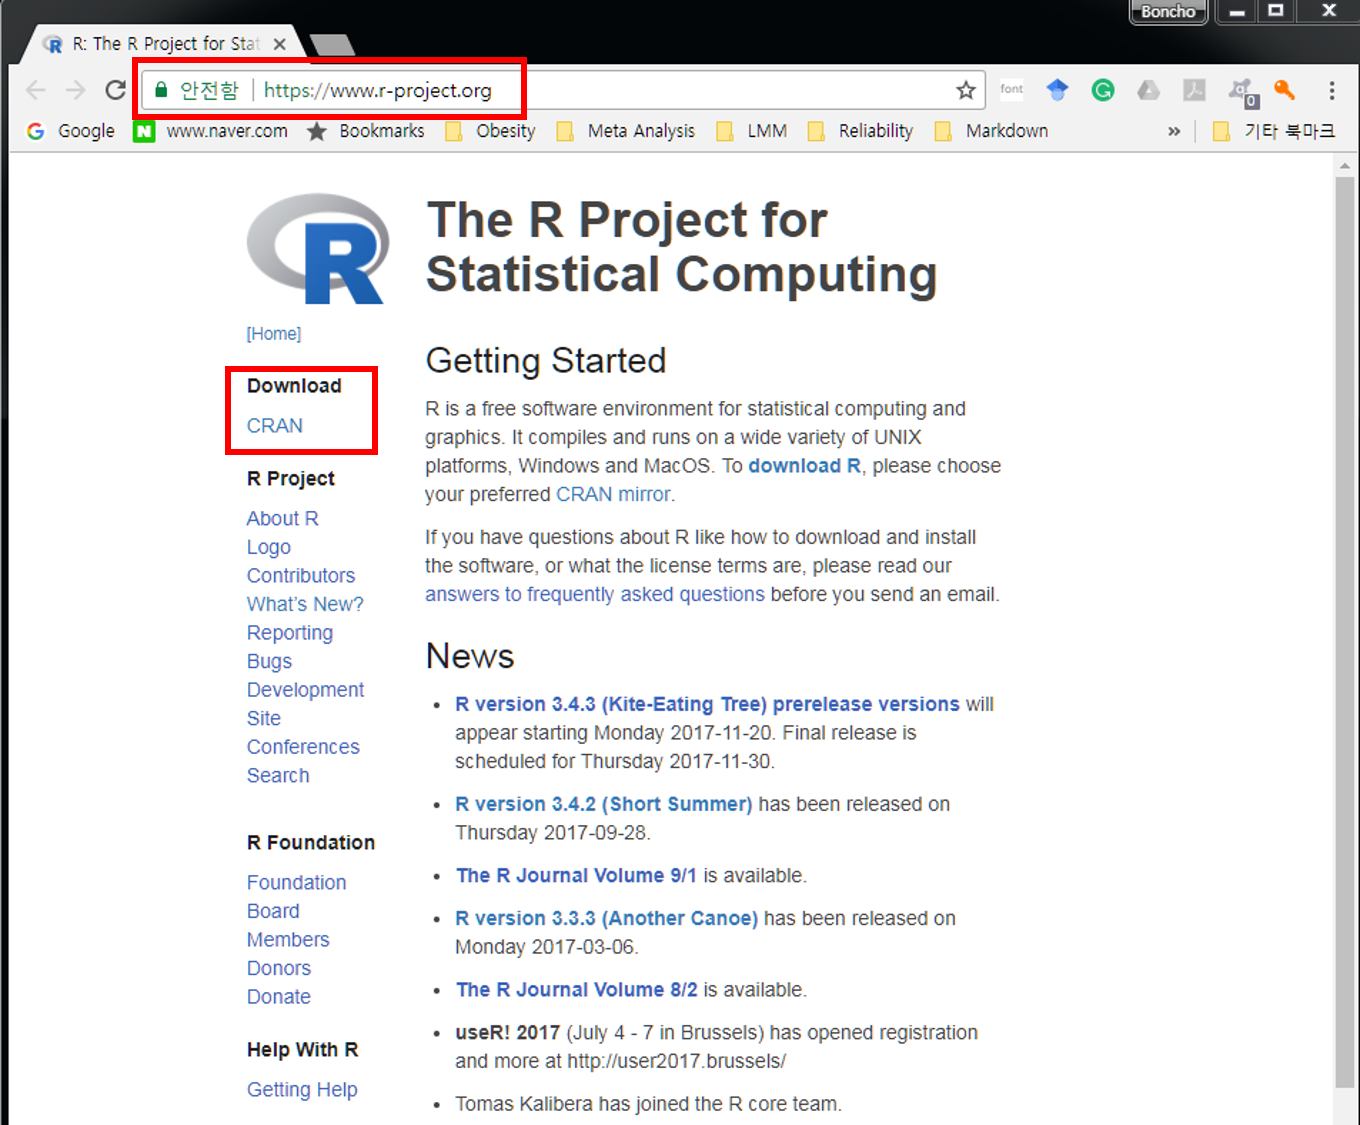
\includegraphics[width = 12cm, height = 12cm]{Figures/Rorg-main-add.png}
  \caption[www.r-project.org 메인화면]{www.r-project.org 메인화면}\label{fig:R-install-01}
}
\end{figure}

\begin{enumerate}
\def\labelenumi{\arabic{enumi}.}
\setcounter{enumi}{2}
\tightlist
\item
  클릭 후 연결한 페이지를 스크롤 후 ``Korea'' 아래 링크 클릭 (그림
  \ref{fig:R-install-02} 참조)
\end{enumerate}

\begin{figure}[H]
{
  \centering
  
\includegraphics[width = 12cm, height = 8cm]{Figures/CRAN-korea-01.PNG}
  \caption[CRAN 국가별 mirrors]{CRAN 국가별 mirrors}\label{fig:R-install-02}
}
\end{figure}

\begin{enumerate}
\def\labelenumi{\arabic{enumi}.}
\setcounter{enumi}{3}
\tightlist
\item
  클릭 후 세 가지 운영체제(Linux, Mac OS X, Windowns)에 따른 R 버전 선택
  가능

  \begin{itemize}
  \tightlist
  \item
    본 문서에서는 Windows 버전 설치만 다룸
  \end{itemize}
\end{enumerate}

\begin{figure}[H]
{
  \centering
  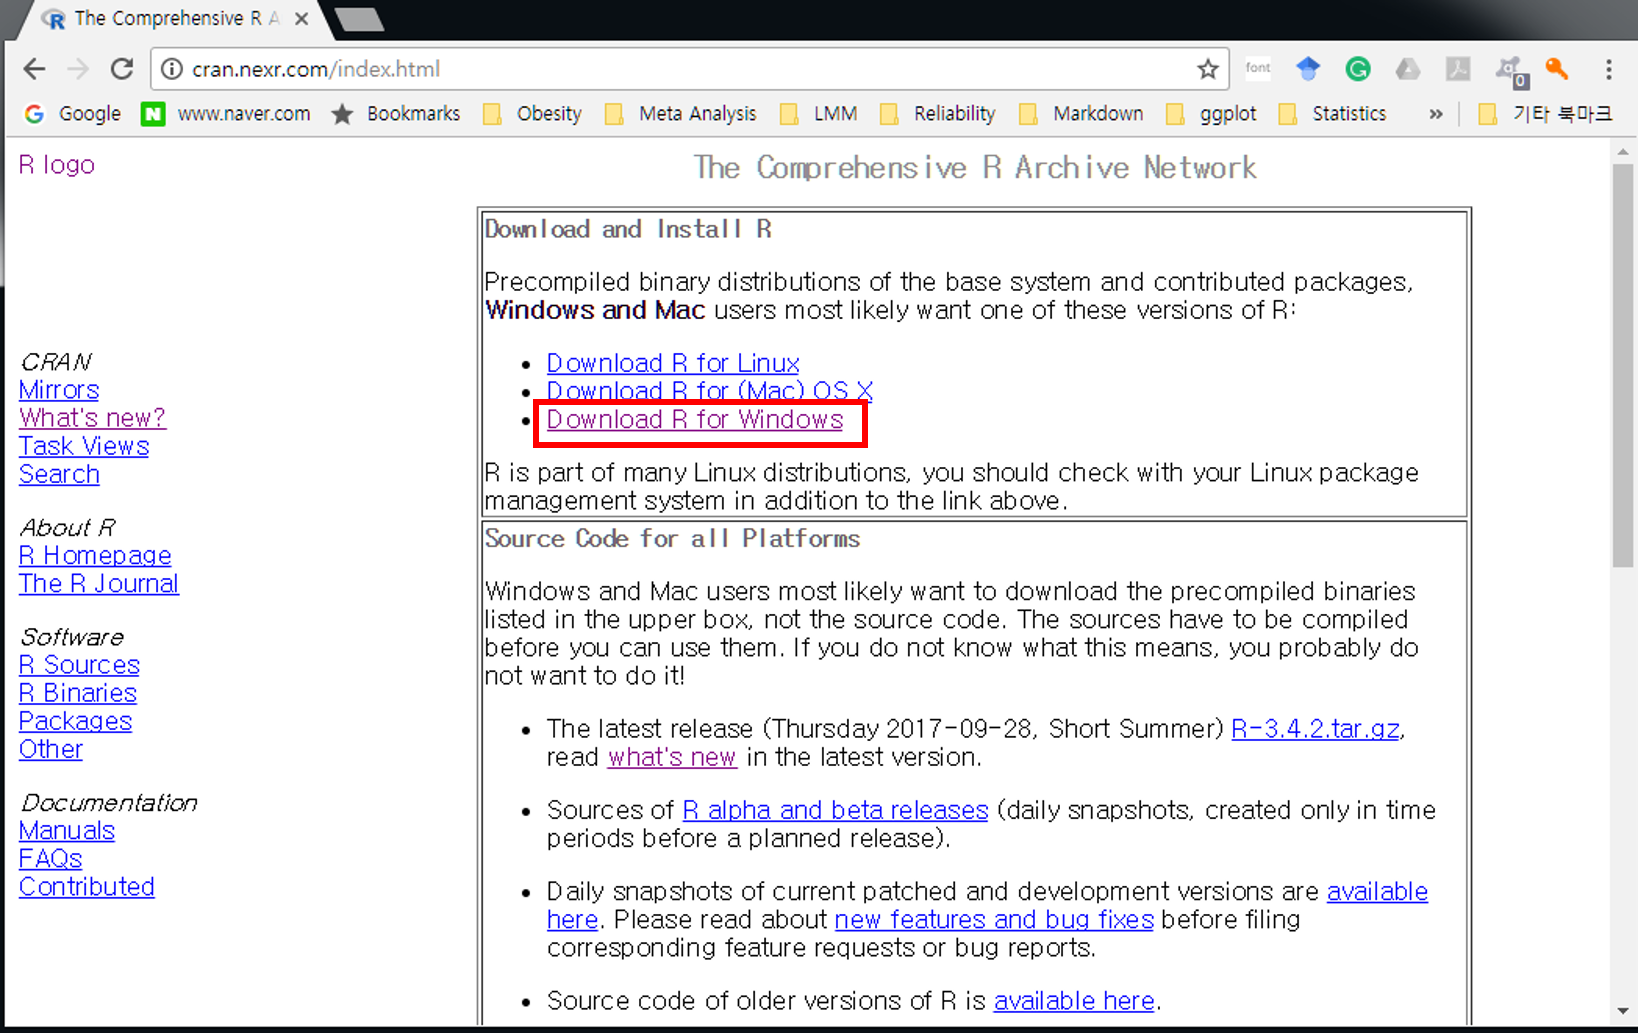
\includegraphics[width = 12cm, height = 10cm]{Figures/Rinstall-01.png}
  \caption[운영체제 별 R 버전 선택]{운영체제 별 R 버전 선택}\label{fig:R-install-03}
}
\end{figure}

\begin{enumerate}
\def\labelenumi{\arabic{enumi}.}
\setcounter{enumi}{4}
\tightlist
\item
  ``Downloads R for Windows'' 링크 클릭하면 다음과 같은 화면으로 이동
\end{enumerate}

\begin{figure}[H]
{
  \centering
  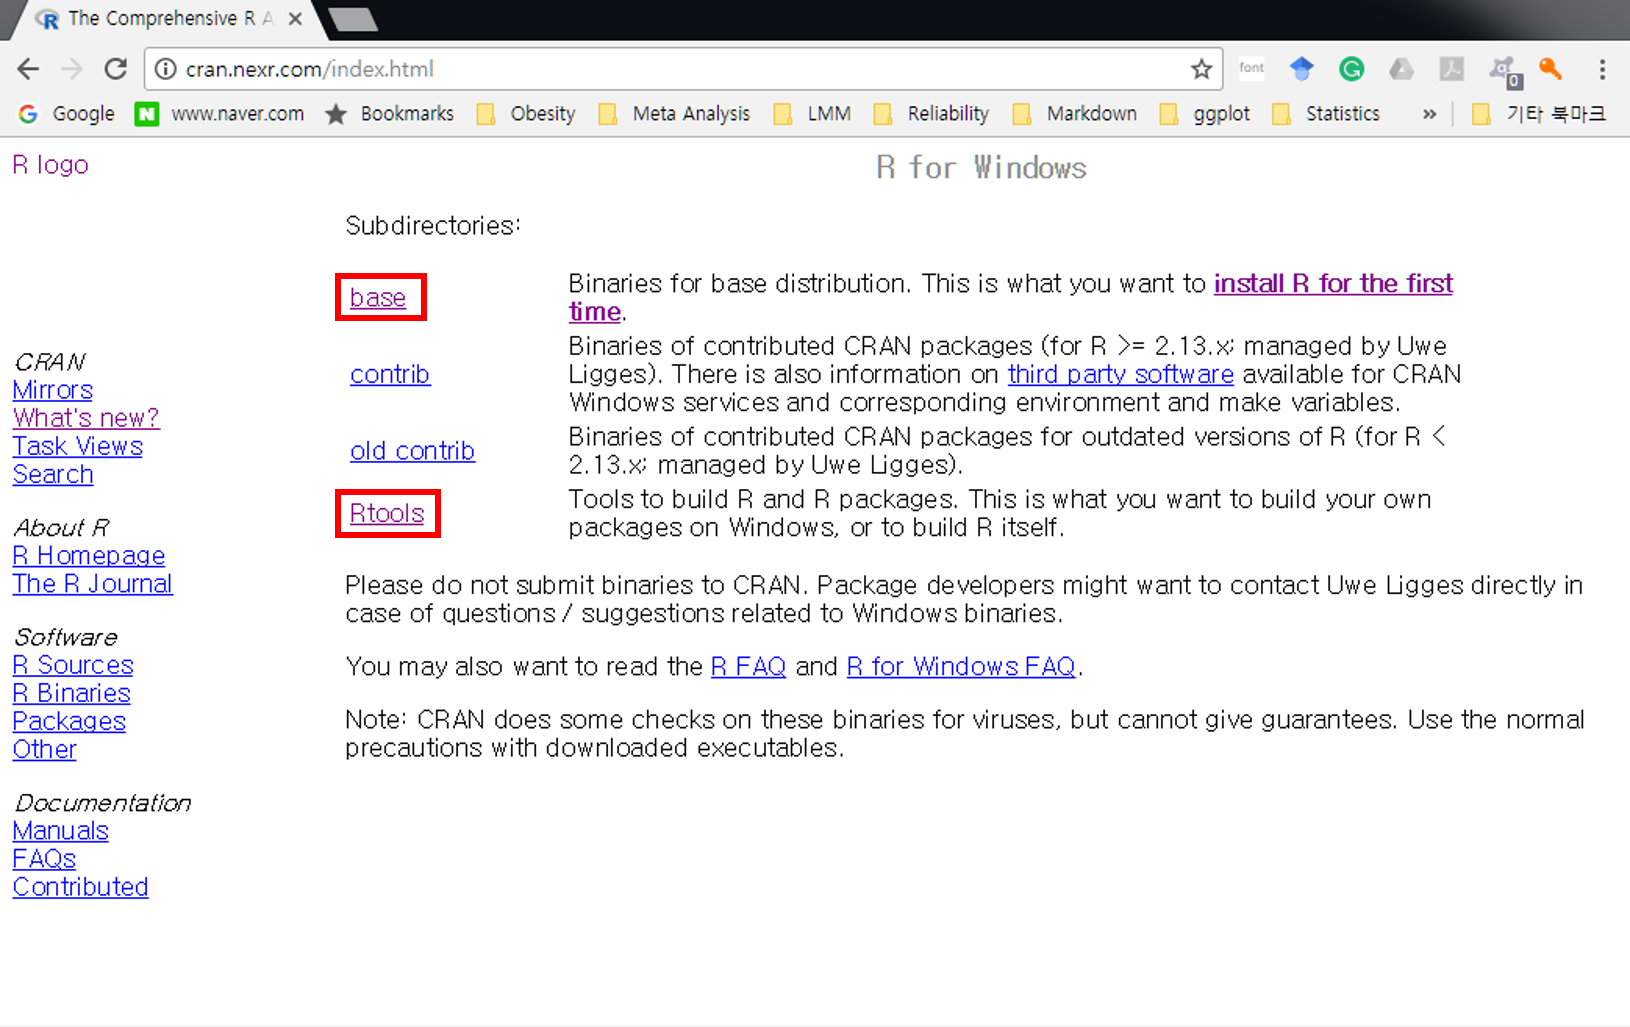
\includegraphics[width = 12cm, height = 10cm]{Figures/Rinstall-02.png}
  \caption[Windows 용 R base 및 구성요소 다운로드]{Windows 용 R base 및 구성요소 다운로드}\label{fig:R-install-04}
}
\end{figure}

\begin{enumerate}
\def\labelenumi{\arabic{enumi}.}
\setcounter{enumi}{5}
\item
  R을 구성하는 하위구조 중 ``base'' 링크 클릭 후 다음 화면에서 가장
  최신버전2017-11-20 현재 ``Downloads R 3.4.2 for Windows'')를 클릭 후
  설치 파일을 임의의 디렉토리에 저장 후 실행(그림 \ref{fig:R-install-05}
  참조)
\item
  참고로 3개 subdirectories에 대한 간략한 설명은 아래와 같음

  \begin{itemize}
  \tightlist
  \item
    \texttt{base}: R 실행 프로그램
  \item
    \texttt{contrib}: R package의 바이너리 파일
  \item
    \texttt{Rtools}: R package 개발 및 배포를 위한 프로그램
  \end{itemize}
\end{enumerate}

\begin{figure}[H]
{
  \centering
  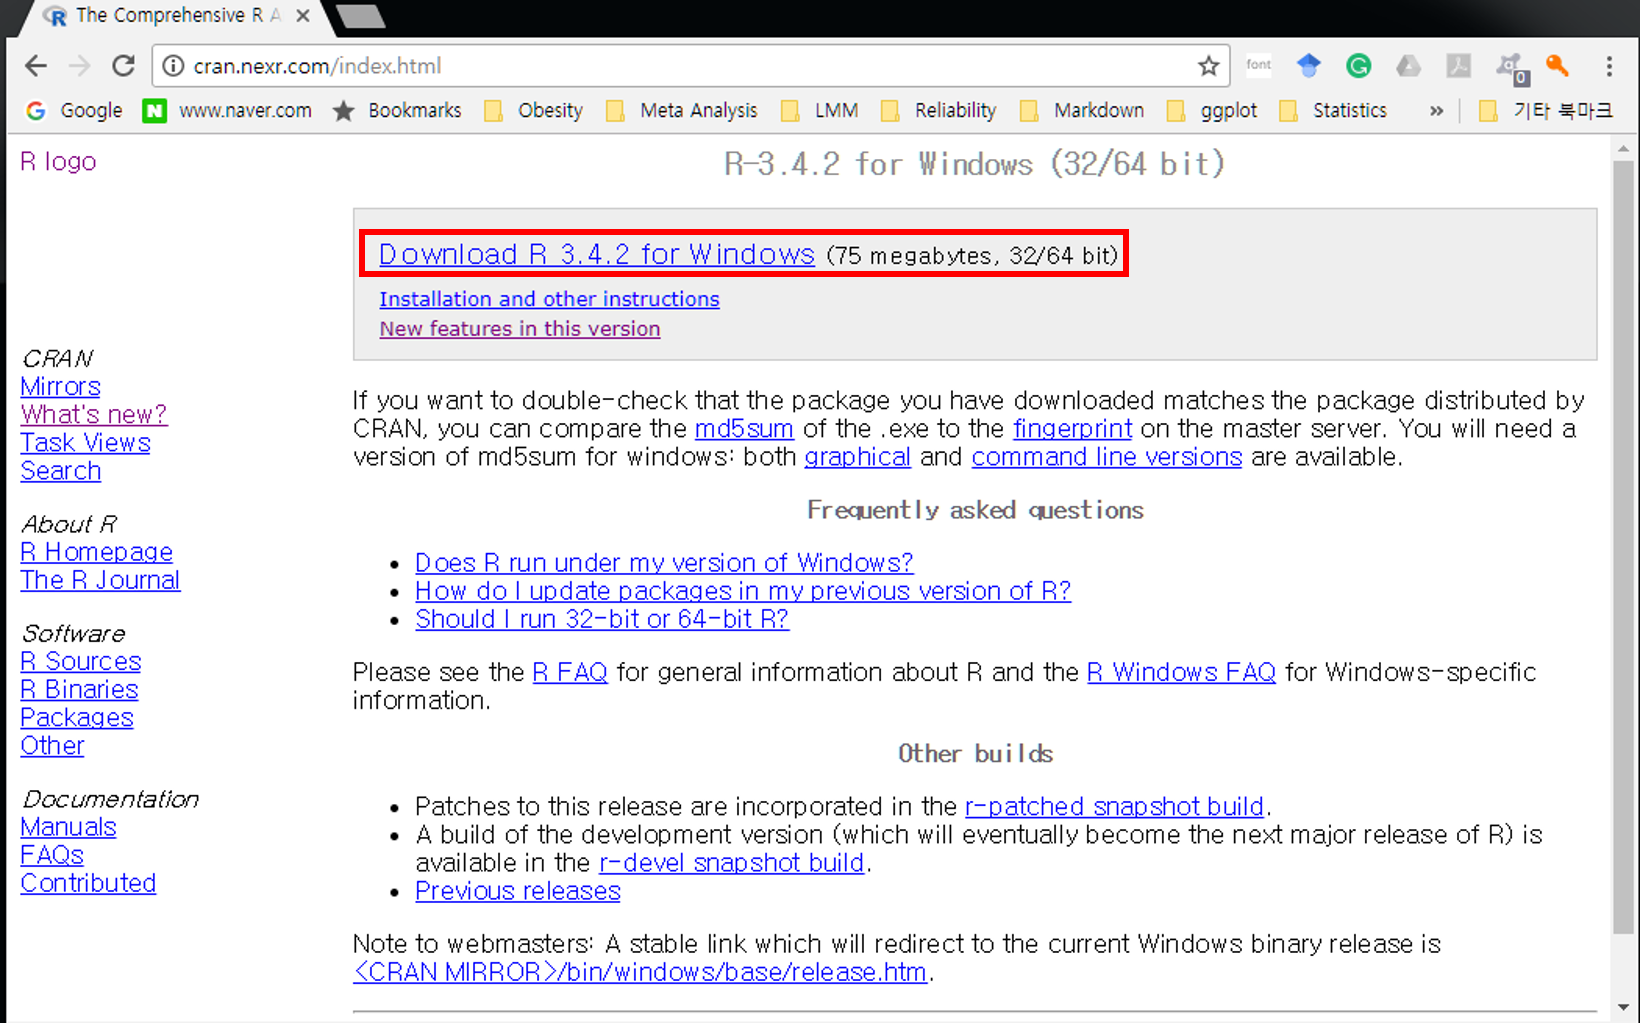
\includegraphics[width = 12cm, height = 10cm]{Figures/Rinstall-03.png}
  \caption[Windows 용 R 설치 파일 다운로드 페이지]{Windows 용 R 설치 파일 다운로드 페이지}\label{fig:R-install-05}
}
\end{figure}

\begin{enumerate}
\def\labelenumi{\arabic{enumi}.}
\setcounter{enumi}{7}
\tightlist
\item
  다운로드한 파일을 실행하면 아래와 같은 대화창이 나타남

  \begin{itemize}
  \tightlist
  \item
    한국어 선택 \(\rightarrow\) 환영 화면에서
    {[}다음(N)\textgreater{}{]} 클릭
  \end{itemize}
\end{enumerate}

\begin{figure}[H]
{
  \centering
  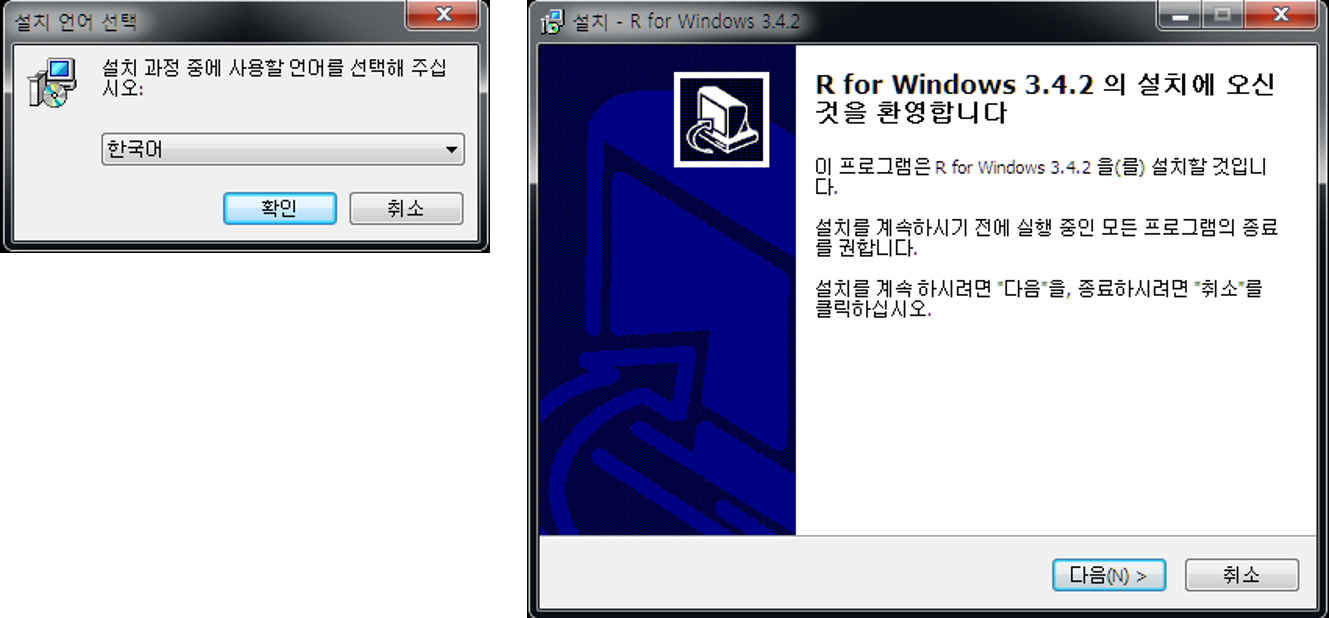
\includegraphics[width = 14cm, height = 11cm]{Figures/R-install-F01.png}
  \caption[R 설치과정 01]{R 설치과정 01}\label{fig:R-install-06}
}
\end{figure}

\begin{enumerate}
\def\labelenumi{\arabic{enumi}.}
\setcounter{enumi}{8}
\tightlist
\item
  GNU 라이센스에 대한 설명 및 동의 여부({[}다음(N)\textgreater{}{]})
  클릭 (그림 \ref{fig:R-install-07})
\end{enumerate}

\begin{figure}[H]
{
  \centering
  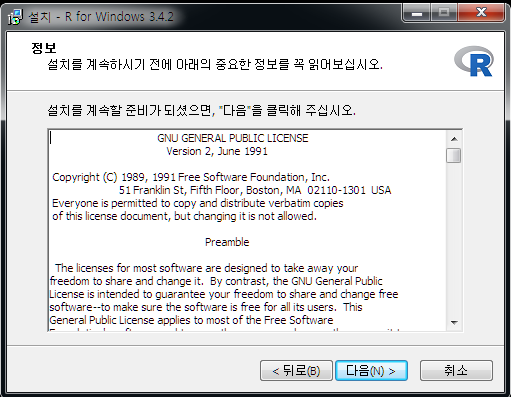
\includegraphics[width = 8cm, height = 8cm]{Figures/R-install-F02.png}
  \caption[R GNU general license]{R GNU general license}\label{fig:R-install-07}
}
\end{figure}

\begin{enumerate}
\def\labelenumi{\arabic{enumi}.}
\setcounter{enumi}{9}
\tightlist
\item
  설치 디렉토리 설정 및 구성요소 설지 여부

  \begin{itemize}
  \tightlist
  \item
    원하는 디렉토리 설정(예:
    \texttt{C:\textbackslash{}R\textbackslash{}R-3.4.2}) (그림
    \ref{fig:R-install-08})
  \item
    기본 프로그램(``Core Files''), 32 또는 64 bit 용 설치 파일, R
    console 한글 번역 모두 체크 뒤 {[}다음(N)\textgreater{}{]} 클릭
    (그림 \ref{fig:R-install-09})
  \end{itemize}
\end{enumerate}

\begin{figure}[H]
{
  \centering
  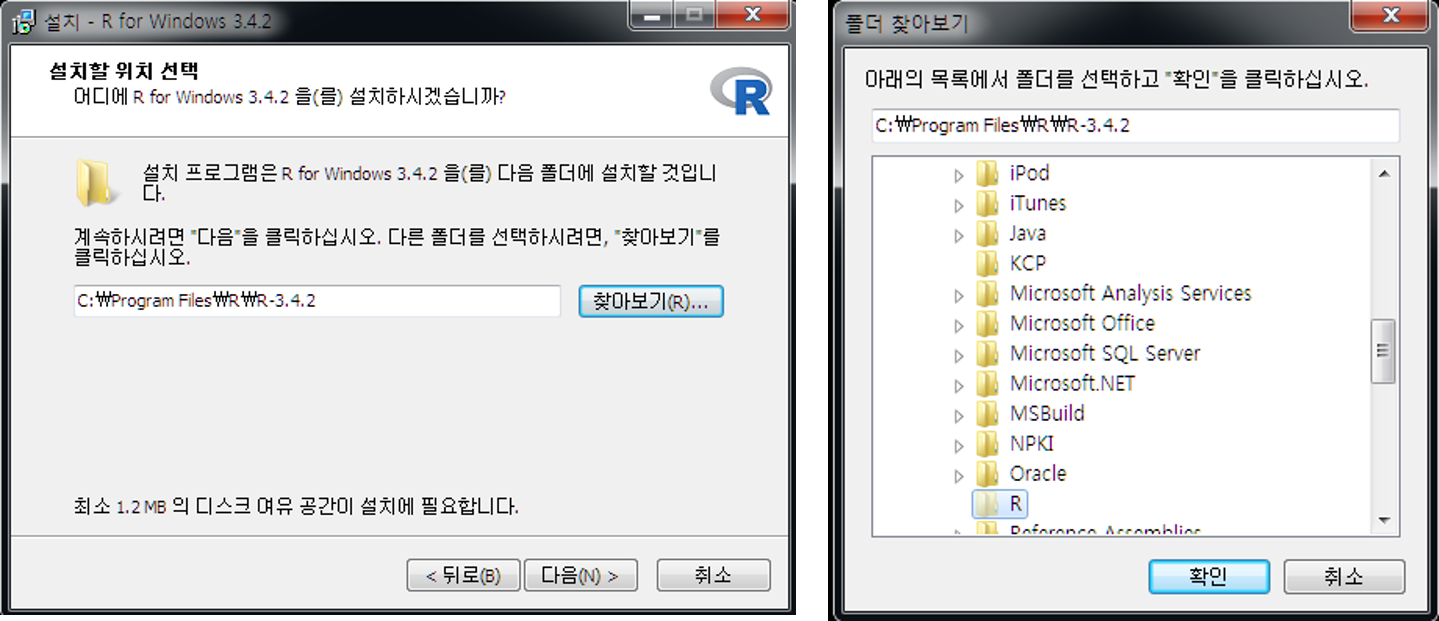
\includegraphics[width = 15cm, height = 10cm]{Figures/R-install-F03.png}
  \caption[R 설치 디렉토리 설정]{R 설치 디렉토리 설정}\label{fig:R-install-08}
}
\end{figure}

\begin{figure}[H]
{
  \centering
  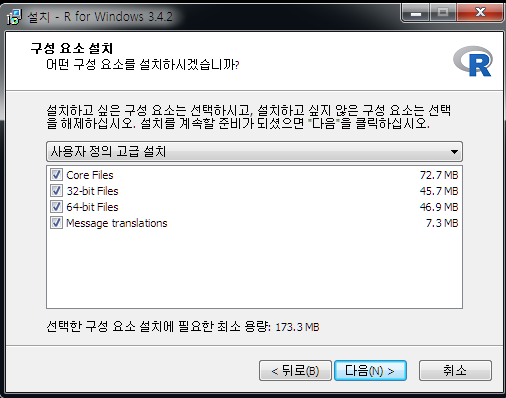
\includegraphics[width = 8cm, height = 8cm]{Figures/R-install-F04.png}
  \caption[R 구성요소 설치]{R 구성요소 설치}\label{fig:R-install-09}
}
\end{figure}

\begin{enumerate}
\def\labelenumi{\arabic{enumi}.}
\setcounter{enumi}{10}
\tightlist
\item
  R 스타트업 옵션 지정

  \begin{itemize}
  \tightlist
  \item
    기본값(``No'' check-button)으로도 설치 진행 가능
  \item
    본 문서에서는 스타트업 옵션 변경으로 진행
  \end{itemize}
\end{enumerate}

\begin{figure}[H]
{
  \centering
  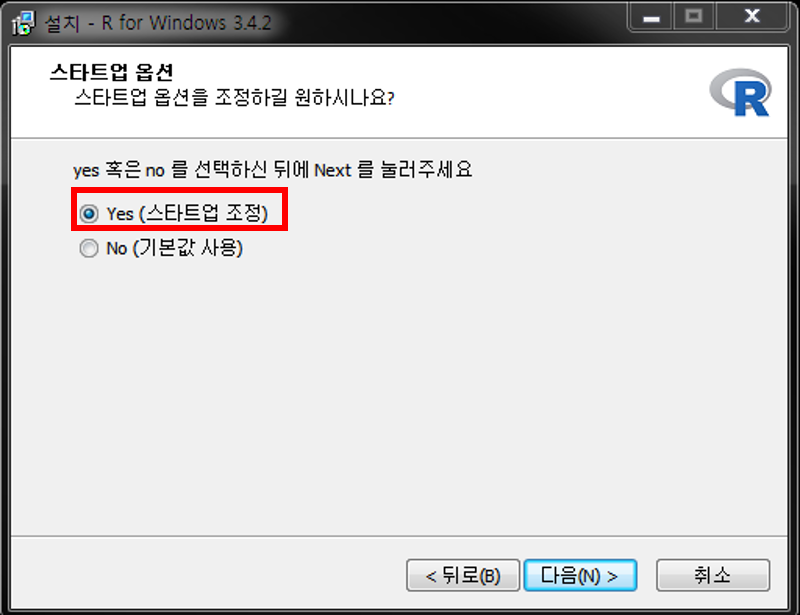
\includegraphics[width = 8cm, height = 8cm]{Figures/R-install-F05.png}
  \caption[R 스타트업 옵션 변경]{R 스타트업 옵션 변경}\label{fig:R-install-10}
}
\end{figure}

\begin{enumerate}
\def\labelenumi{\arabic{enumi}.}
\setcounter{enumi}{11}
\tightlist
\item
  화면표시방식(디스플레이 모드) 설정 변경

  \begin{itemize}
  \tightlist
  \item
    MDI: 한 윈도우 내에서 script 편집창, 출력, 도움말 창 사용
  \item
    SDI: 다중 창에서 각각 script 편집창, 출력, 도움말 등을 독립적으로
    열기
  \end{itemize}
\end{enumerate}

\begin{figure}[H]
{
  \centering
  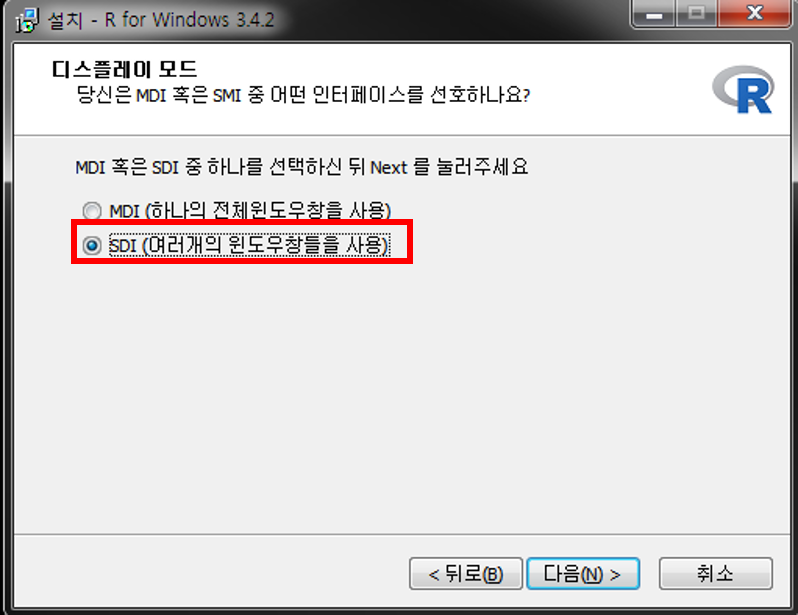
\includegraphics[width = 8cm, height = 8cm]{Figures/R-install-F06.png}
  \caption[R 화면표시방식 설정 변경]{R 화면표시방식 설정 변경}\label{fig:R-install-11}
}
\end{figure}

\begin{enumerate}
\def\labelenumi{\arabic{enumi}.}
\setcounter{enumi}{12}
\tightlist
\item
  도움말 형식에서 HTML 도움말 기반 선택
\end{enumerate}

\begin{figure}[H]
{
  \centering
  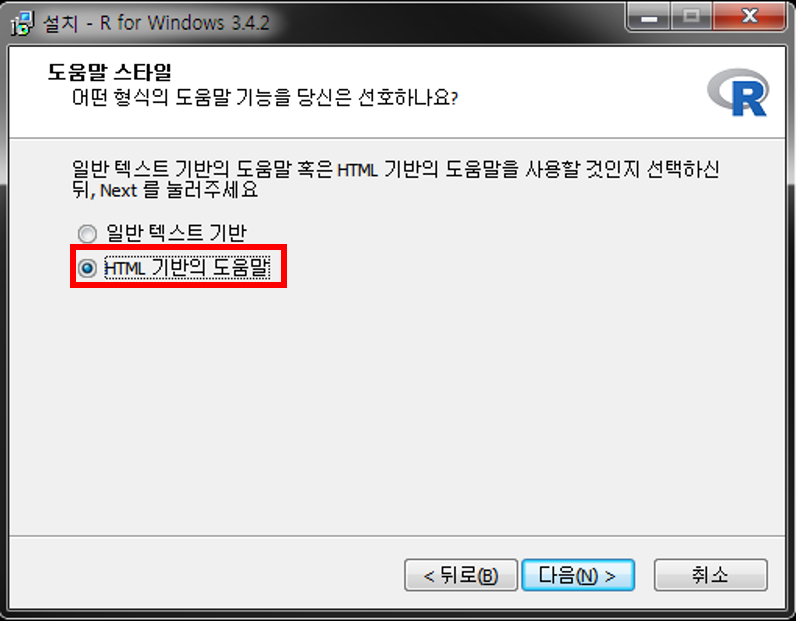
\includegraphics[width = 8cm, height = 8cm]{Figures/R-install-F07.png}
  \caption[R 도움말 형식 변경]{R 도움말 형식 변경}\label{fig:R-install-12}
}
\end{figure}

\begin{enumerate}
\def\labelenumi{\arabic{enumi}.}
\setcounter{enumi}{13}
\tightlist
\item
  시작메뉴 폴더 선택(그림 \ref{fig:R-install-13})

  \begin{itemize}
  \tightlist
  \item
    ``바로가기''를 생성할 시작 메뉴 폴더 지정 후
    {[}다음(N)\textgreater{}{]} 클릭 후 설치 진행
  \item
    하단 ``시작메뉴 폴더 만들지 않음'' 체크박스 표시 시 시작메뉴에
    ``바로가기'' 생성되지 않음(실행에 전혀 지장 없음)
  \end{itemize}
\end{enumerate}

\begin{figure}[H]
{
  \centering
  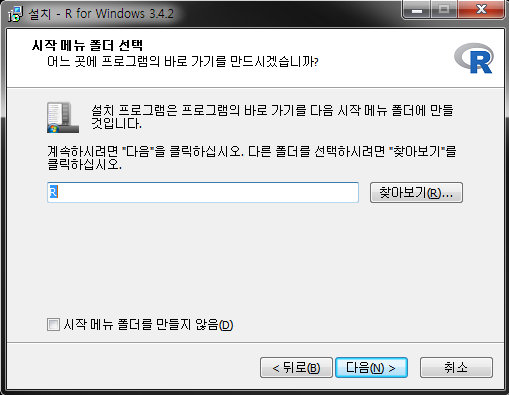
\includegraphics[width = 8cm, height = 8cm]{Figures/R-install-F08.png}
  \caption[시작메뉴 폴더 선택]{시작메뉴 폴더 선택}\label{fig:R-install-13}
}
\end{figure}

\begin{enumerate}
\def\labelenumi{\arabic{enumi}.}
\setcounter{enumi}{14}
\tightlist
\item
  추가 옵션 지정: 바탕화면 아이콘 생성 등 추가적 작업 옵션 체크 후
  {[}다음(N)\textgreater{}{]} 클릭 \(\rightarrow\) 설치 진행

  \begin{itemize}
  \tightlist
  \item
    설치된 R 버전 정보 레지스트리 저장 여부
  \item
    \texttt{.Rdata} 확장자를 R 실행파일과 자동 연계
  \end{itemize}
\end{enumerate}

\begin{figure}[H]
{
  \centering
  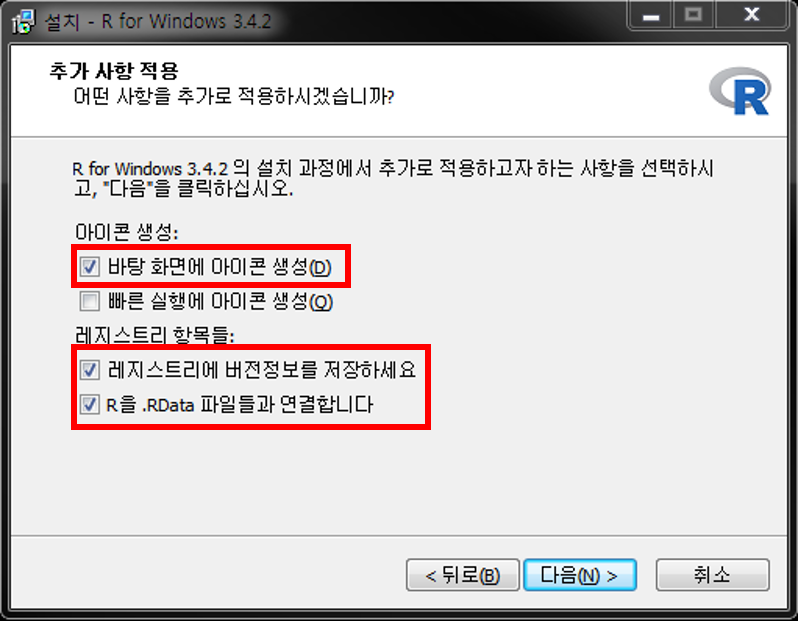
\includegraphics[width = 8cm, height = 8cm]{Figures/R-install-F09.png}
  \caption[R 추가옵션 사항 선택]{R 추가옵션 사항 선택}\label{fig:R-install-14}
}
\end{figure}

\begin{enumerate}
\def\labelenumi{\arabic{enumi}.}
\setcounter{enumi}{15}
\tightlist
\item
  설치 완료 후 바탕화면의 R 아이콘을 더블클릭하면 Rgui가 실행
\end{enumerate}

\begin{figure}[H]
{
  \centering
  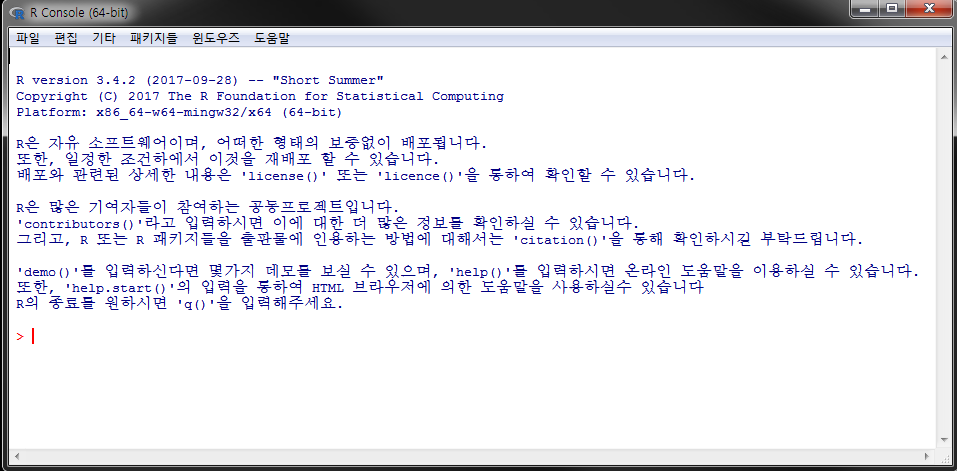
\includegraphics[width = 15cm, height = 10cm]{Figures/Rgui.png}
  \caption[Windows에서 R 실행화면(SDI)]{Windows에서 R 실행화면(콘솔 창, SDI 모드)}\label{fig:R-install-15}
}
\end{figure}

\section{R 시작 및 작동 체크}\label{r----}

위 R 시작화면에서 간단한 명령어들을 체크

\begin{itemize}
\tightlist
\item
  그림 \ref{fig:R-install-15}에서 \texttt{\textgreater{}} 기호는 R의
  명령 프롬프트임.
\item
  Checklist

  \begin{enumerate}
  \def\labelenumi{\arabic{enumi})}
  \tightlist
  \item
    ``Hello R'' 출력
  \item
    1부터 100까지 정수 출력
  \item
    간단한 histogram 출력
  \end{enumerate}
\end{itemize}

\footnotesize

\begin{Shaded}
\begin{Highlighting}[]
\OperatorTok{>}\StringTok{ }\CommentTok{# 문자열 출력}
\ErrorTok{>}\StringTok{ }\KeywordTok{print}\NormalTok{(}\StringTok{"Hello R"}\NormalTok{)}
\end{Highlighting}
\end{Shaded}

\begin{verbatim}
[1] "Hello R"
\end{verbatim}

\normalsize

여기서 \texttt{\#} 기호는 주석의 시작을 의미하며 같은 행에서 \texttt{\#}
뒤 내용의 코드는 실행되지 않음

\footnotesize

\begin{Shaded}
\begin{Highlighting}[]
\OperatorTok{>}\StringTok{ }\CommentTok{# 1부터 100까지 수열 출력}
\ErrorTok{>}\StringTok{ }\KeywordTok{seq}\NormalTok{(}\DecValTok{1}\OperatorTok{:}\DecValTok{100}\NormalTok{)  }\CommentTok{# print('Hello R')}
\end{Highlighting}
\end{Shaded}

\begin{verbatim}
  [1]   1   2   3   4   5   6   7   8   9  10  11  12  13  14  15  16  17  18  19  20
 [21]  21  22  23  24  25  26  27  28  29  30  31  32  33  34  35  36  37  38  39  40
 [41]  41  42  43  44  45  46  47  48  49  50  51  52  53  54  55  56  57  58  59  60
 [61]  61  62  63  64  65  66  67  68  69  70  71  72  73  74  75  76  77  78  79  80
 [81]  81  82  83  84  85  86  87  88  89  90  91  92  93  94  95  96  97  98  99 100
\end{verbatim}

\normalsize

\footnotesize

\begin{Shaded}
\begin{Highlighting}[]
\OperatorTok{>}\StringTok{ }\CommentTok{# 간단한 히스토그램}
\ErrorTok{>}\StringTok{ }\KeywordTok{set.seed}\NormalTok{(}\DecValTok{12345}\NormalTok{)  }\CommentTok{# random seed 지정}
\OperatorTok{>}\StringTok{ }\NormalTok{x <-}\StringTok{ }\KeywordTok{rnorm}\NormalTok{(}\DecValTok{1000}\NormalTok{)  }\CommentTok{# 평균 0, 분산 1인 정규분포에서 난수 1000개 생성}
\OperatorTok{>}\StringTok{ }\KeywordTok{hist}\NormalTok{(x)  }\CommentTok{# 히스토그램}
\end{Highlighting}
\end{Shaded}

\begin{center}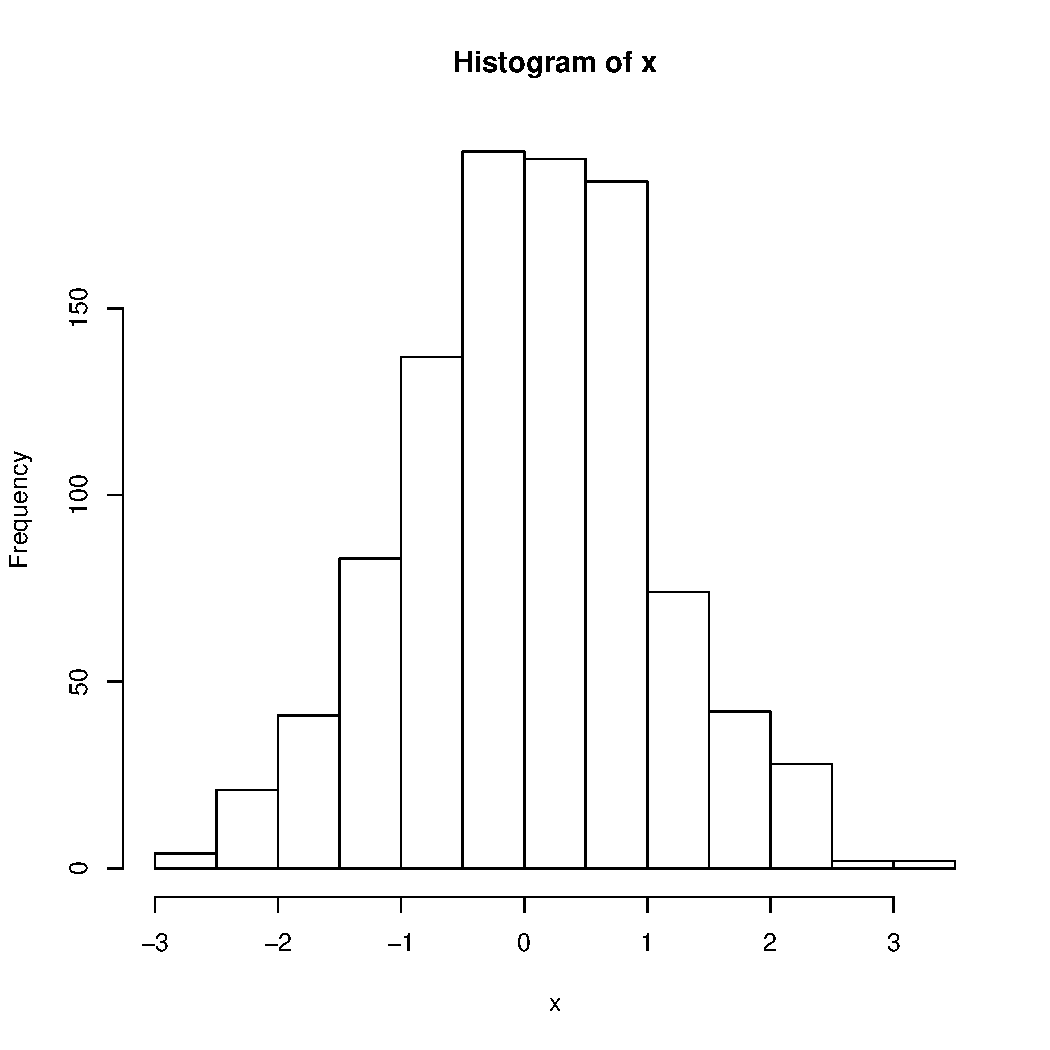
\includegraphics[width=10 cm,height=10 cm]{Figures/check-03-1} \end{center}

\normalsize

\begin{quote}
\colorbox{gray!10}{\begin{minipage}{15cm}
\textbf{Tips}

R 명령어 실행 시 간혹 아니 매우 빈번히 오류가 나타나는데, 이를 해결할 수 있는 가장 손쉬운 방법은 Googling과 R의 도움말을 이용하는 것이 가장 효율적임. 
\end{minipage}}
\end{quote}

도움말을 볼 수 있은 R 함수 리스트

\begin{table}[H]
  \centering
  \begingroup\footnotesize
  \caption{R help 관련 명령어 리스트}
  \begin{tabular}{p{3cm}p{5cm}p{7cm}}
  \toprule
  \textbf{도움말 보기 명령어} & \textbf{설명} & \textbf{사용법} \\
  \midrule
  \texttt{help} 또는 \texttt{?}          & 도움말 시스템 호출               & \texttt{help(topic \textit{\# 도움말을 찾고자 하는 대상 또는 함수}) }\\
  \texttt{help.search} 또는 \texttt{??}  & 주어진 문자열을 포함한 문서 검색 & \texttt{help.search(pattern \textit{\# 찾고자 하는 문자열})} \\ 
  \texttt{example}                       & topic의 도움말 페이지에 있는 examples section 실행 & \texttt{example(topic \textit{\# 예제를 실행하고자 하는 topic 또는 함수})} \\
  \texttt{vignette}                      & topic의 pdf 또는 html 레퍼런스 메뉴얼 불러오기 & \texttt{vignette(topic \textit{\# topic에 저장된 reference manual})} \\
  \bottomrule
  \end{tabular}
  \endgroup
\end{table}

\begin{quote}
\colorbox{gray!10}{\begin{minipage}{15cm}
\textbf{Tips}
\begin{itemize}
\item \texttt{vignette}에서 제공하는 문서는 실제 분석을 기반으로 작성한 문서이기 때문에 초보자들이 R 패키지의 접근성을 높혀줌. \texttt{browseVignettes()}으로 현존하는 모든 R 패키지들의 vignette을 볼 수 있기 때문에 매우 유용함.
\item R 세션(R 콘솔이 시작해서 종료까지)에 설정된 옵션은 \texttt{options()} 실행으로 확인 가능
\item 현재 R 세션에 대한 정보는 \texttt{sessionInfo()} 함수로 확인 가능
\end{itemize}
\end{minipage}}
\end{quote}

\emph{참고}

\footnotesize

\begin{Shaded}
\begin{Highlighting}[]
\OperatorTok{>}\StringTok{ }\CommentTok{# 현재 설정된 출력 자리수 확인}
\ErrorTok{>}\StringTok{ }\KeywordTok{options}\NormalTok{(}\StringTok{"digits"}\NormalTok{)}
\end{Highlighting}
\end{Shaded}

\begin{verbatim}
$digits
[1] 7
\end{verbatim}

\begin{Shaded}
\begin{Highlighting}[]
\OperatorTok{>}\StringTok{ }\NormalTok{pi}
\end{Highlighting}
\end{Shaded}

\begin{verbatim}
[1] 3.141593
\end{verbatim}

\begin{Shaded}
\begin{Highlighting}[]
\OperatorTok{>}\StringTok{ }\CommentTok{# 출력 자리수를 7에서 3으로 변경}
\ErrorTok{>}\StringTok{ }\KeywordTok{options}\NormalTok{(}\DataTypeTok{digits =} \DecValTok{3}\NormalTok{)}
\OperatorTok{>}\StringTok{ }\NormalTok{pi}
\end{Highlighting}
\end{Shaded}

\begin{verbatim}
[1] 3.14
\end{verbatim}

\normalsize

\subsection{이것으로 R 설치 완료??}\label{-r--}

\begin{itemize}
\tightlist
\item
  기본적 R 사용방식은 입력한 명령어와 실행결과를 확인하는
  대화형(interpreter) 방식
\item
  R 기본 콘솔창 안에서도 \keystroke{TAB}을 누르면 자동완성 기능이라던가
  \keystroke{$\uparrow$}, \keystroke{$\downarrow$}를 누르면 이전/이후
  명령 기록을 볼 수 있음.
\item
  여러 줄 이상의 R 명령어라든가 반복적, 장기간 작업을 수행해야 하는
  경우라면 R 명령어로 구성된 스크립트 작성 후 일괄 실행하는 것이
  일반적임.
\item
  이러한 다중 명령 코딩 시 콘솔창에 직접 입력하는 것은 비효율적
  \(\rightarrow\) 스크립트 에디터를 주로 사용
\item
  R 자체적으로 기본적인 스크립트 에디터 제공(R editor) \(\rightarrow\)
  가독성 및 코딩 효율이 떨어짐
\item
  대표적 R 에디터: WinEdt (\url{http://www.winedt.com}), Tinn-R
  (\url{https://sourceforge.net/projects/tinn-r/}), Vim
  (\url{http://www.vim.org/scripts/script.php?script_id=2628})
\item
  대부분의 분석 및 개발 환경이 RGUI 만으로 구성되어 있지 않음
  \(\rightarrow\) \textbf{RStudio}를 이용한 통합 분석 환경 설정
\end{itemize}

\newpage

\section{RStudio 설치하기}\label{rstudio-}

\begin{itemize}
\tightlist
\item
  Rstudio: R 통합 분석/개발 환경(integrated development environment,
  IDE)으로 현재 가장 대중적으로 사용되고 있는 R 사용 환경
\item
  명령 콘솔 외 파일 편집, 데이터 보기, 명령 기록(\texttt{.history}),
  그래프 등에 쉽게 접근 가능
\item
  R과 마찬가지로 무료 소프트웨어임
\end{itemize}

\begin{enumerate}
\def\labelenumi{\arabic{enumi}.}
\tightlist
\item
  Rstudio 사이트 접속

  \begin{itemize}
  \tightlist
  \item
    웹 브라우저를 통해 \url{https://www.rstudio.com} 연결 후 메인
    화면에서 ``Download Rstudio'' 클릭
  \item
    혹은 상단 Pop-up 메뉴 중 Products \(\rightarrow\) RStudio 클릭 후
    연결된 화면에서 다운로드 진행
  \end{itemize}
\end{enumerate}

\begin{figure}[H]
{
  \centering
  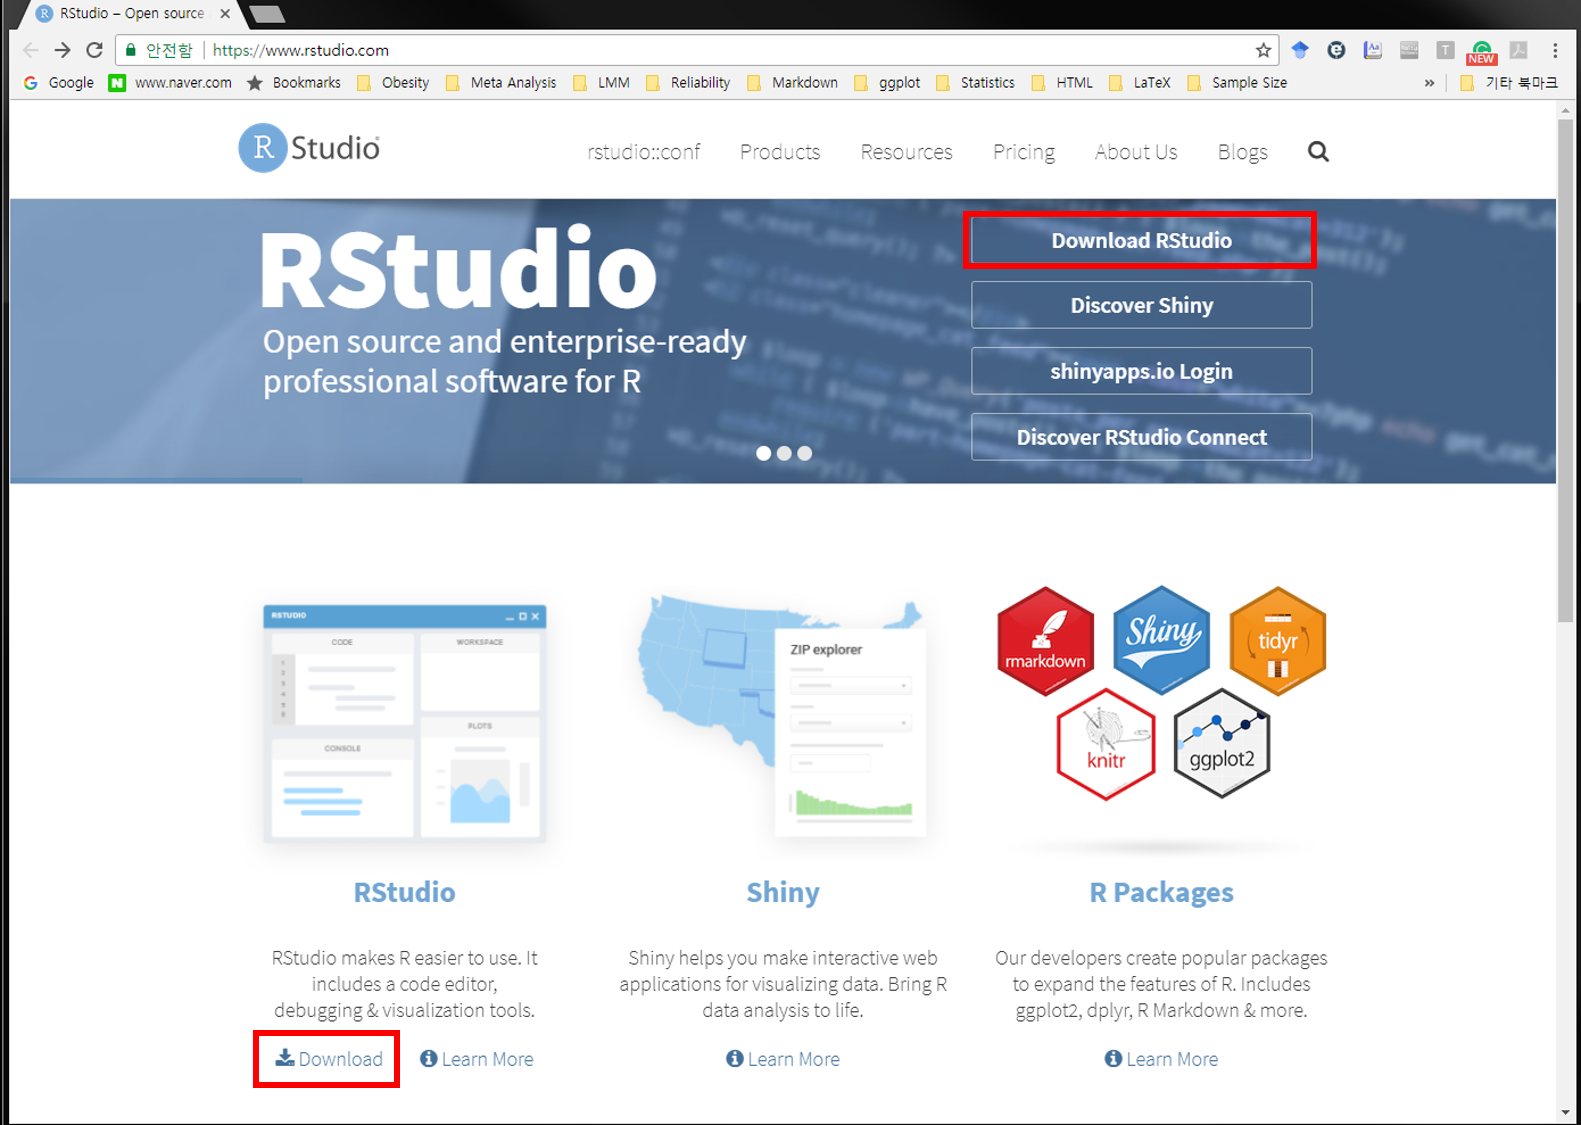
\includegraphics[width = 13cm, height = 13cm]{Figures/Rstudio-main.png}
  \caption[RStudio 메인 페이지]{RStudio 메인 페이지 화면}\label{fig:Rstudio-install-01}
}
\end{figure}

\begin{enumerate}
\def\labelenumi{\arabic{enumi}.}
\setcounter{enumi}{1}
\tightlist
\item
  Desktop 또는 Sever 버전 중 택일

  \begin{itemize}
  \tightlist
  \item
    서버용 설치를 위해서는 Server 클릭 \(\rightarrow\) 소규모 자료
    분석용으로는 불필요
  \item
    여기서는 ``Desktop'' 버전 선택 후 다음 링크로 이동
  \end{itemize}
\end{enumerate}

\begin{figure}[H]
{
  \centering
  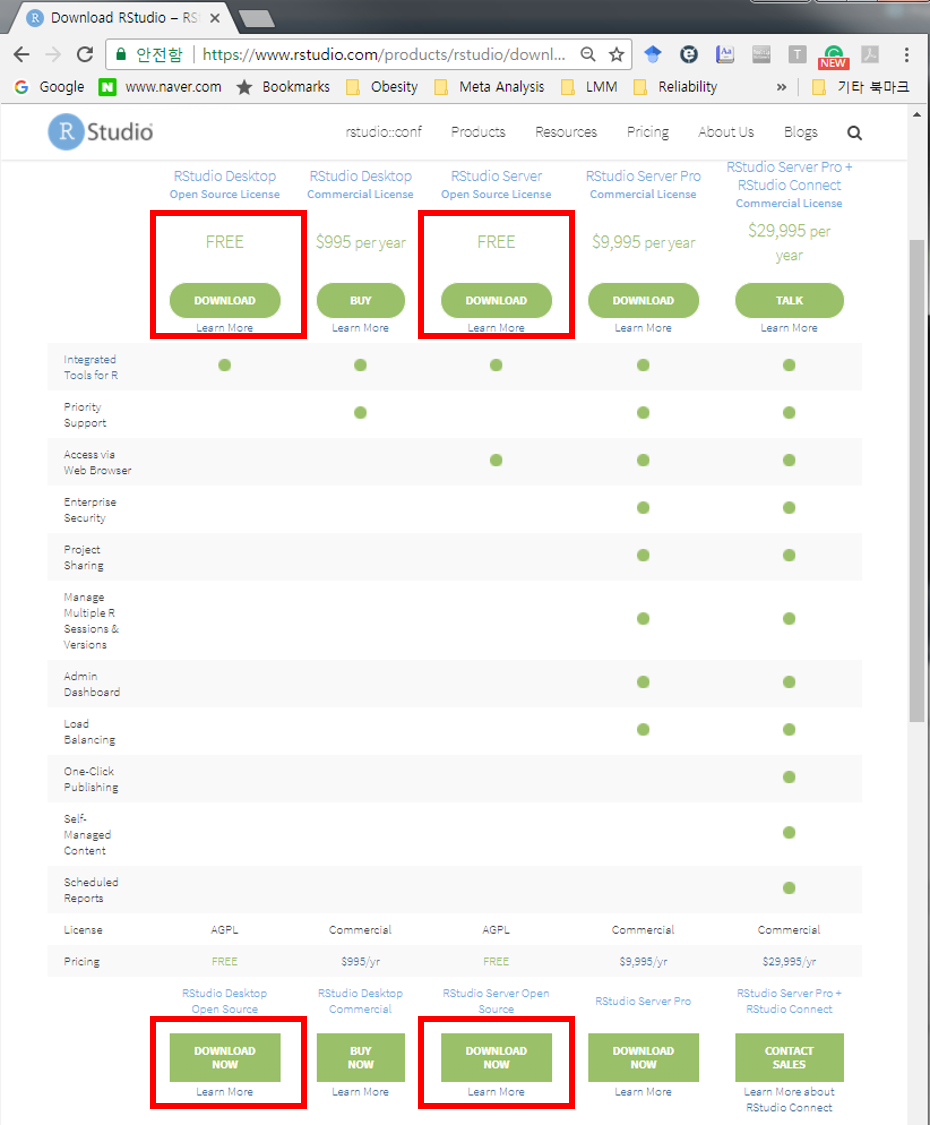
\includegraphics[width = 12cm, height = 10cm]{Figures/Rstudio-download.png}
  \caption[RStudio 다운로드 페이지]{RStudio 다운로드 페이지}\label{fig:Rstudio-install-02}
}
\end{figure}

\begin{enumerate}
\def\labelenumi{\arabic{enumi}.}
\setcounter{enumi}{2}
\tightlist
\item
  운영체제에 맞는 Rstudio installer 다운로드(여기서는 Windows 버전
  다운로드)
\end{enumerate}

\begin{figure}[H]
{
  \centering
  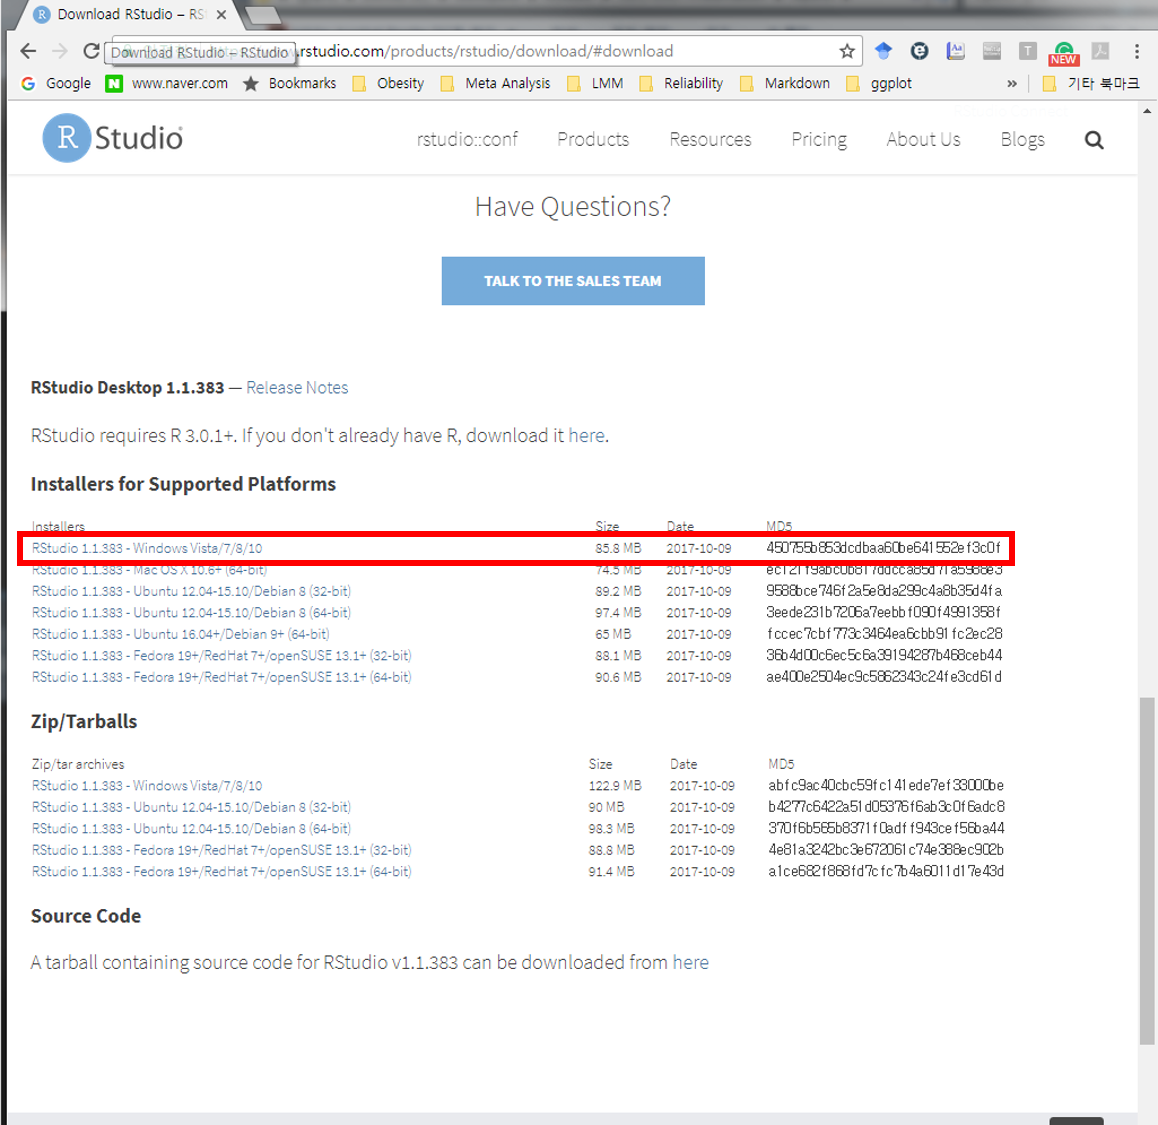
\includegraphics[width = 12cm, height = 10cm]{Figures/Rstudio-download-02.png}
  \caption[RStudio 운영체제 선택]{RStudio 운영체제 선택}\label{fig:Rstudio-install-03}
}
\end{figure}

\begin{enumerate}
\def\labelenumi{\arabic{enumi}.}
\setcounter{enumi}{3}
\tightlist
\item
  RStudio installer 다운로드 시 파일이 저장된 폴더에서 보통
  \texttt{RStudio-xx.xx.xxx.exe} 형식의 파일명 확인

  \begin{itemize}
  \tightlist
  \item
    더블 클릭 후 실행
  \item
    \keystroke{다음>} 몇 번 누르면 설치 종료
  \end{itemize}
\end{enumerate}

\begin{figure}[H]
{
  \centering
  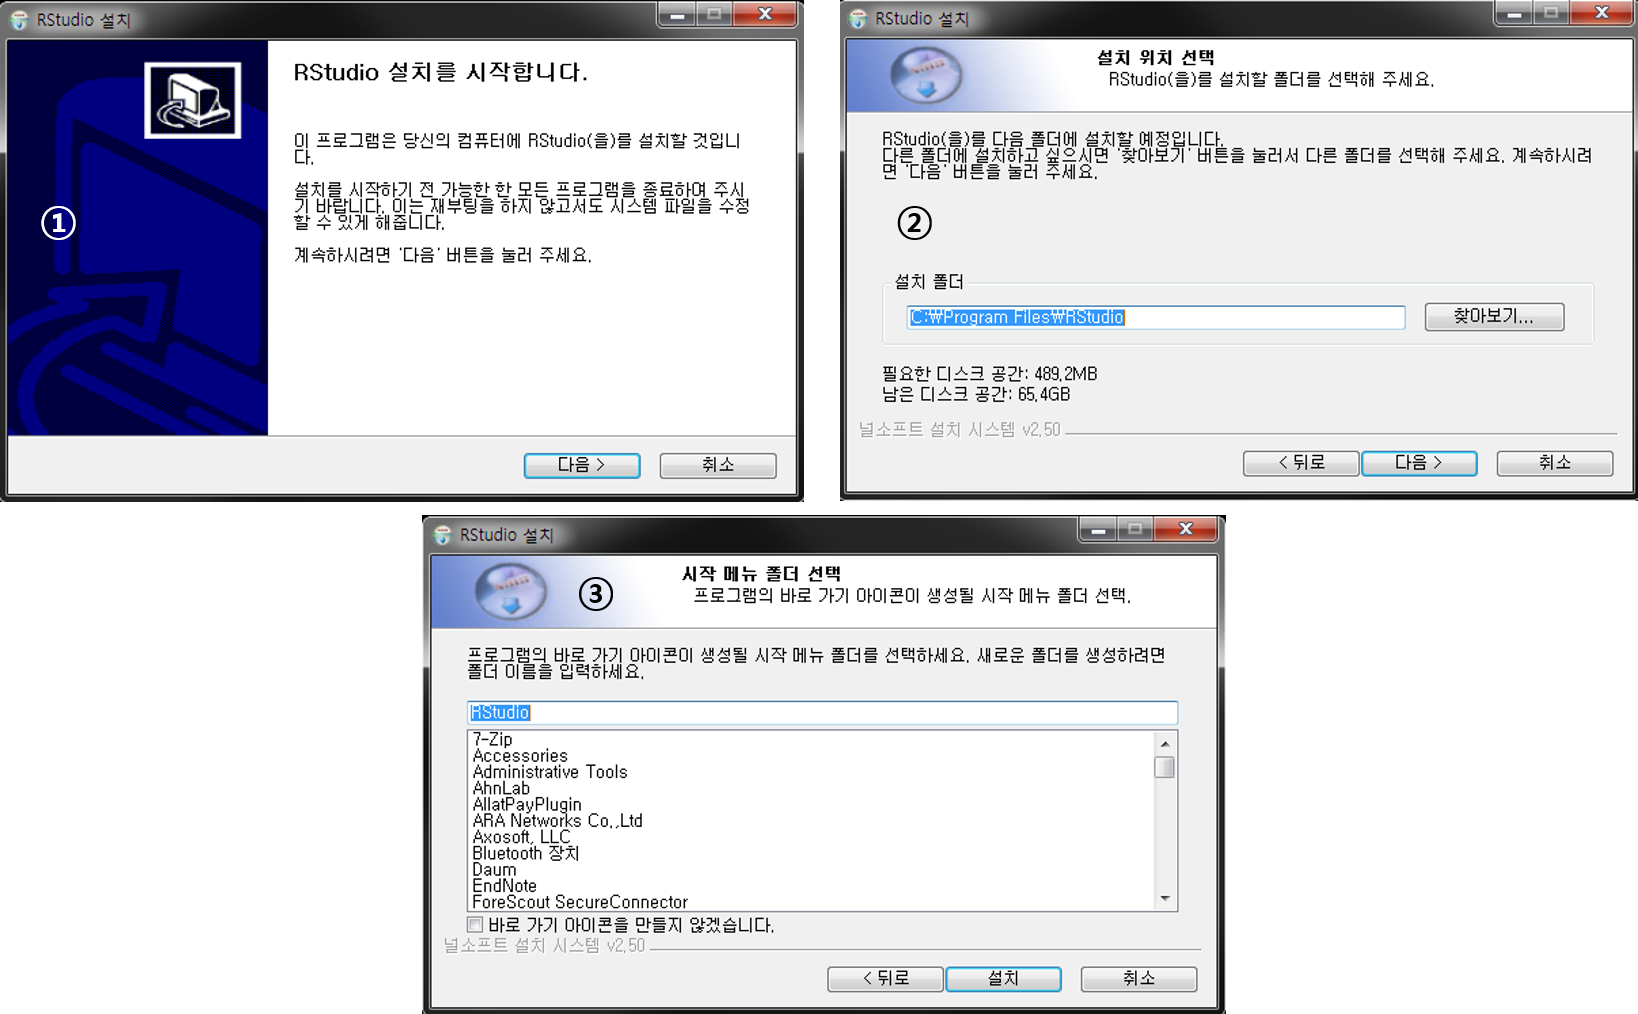
\includegraphics[width = 15cm, height = 12cm]{Figures/Rstudio-installer.png}
  \caption[RStudio 설치화면]{RStudio 설치화면}\label{fig:Rstudio-install-04}
}
\end{figure}

\begin{enumerate}
\def\labelenumi{\arabic{enumi}.}
\setcounter{enumi}{4}
\tightlist
\item
  아래와 같은 실행화면이 나타나면 RStudio 설치 성공
\end{enumerate}

\begin{figure}[H]
{
  \centering
  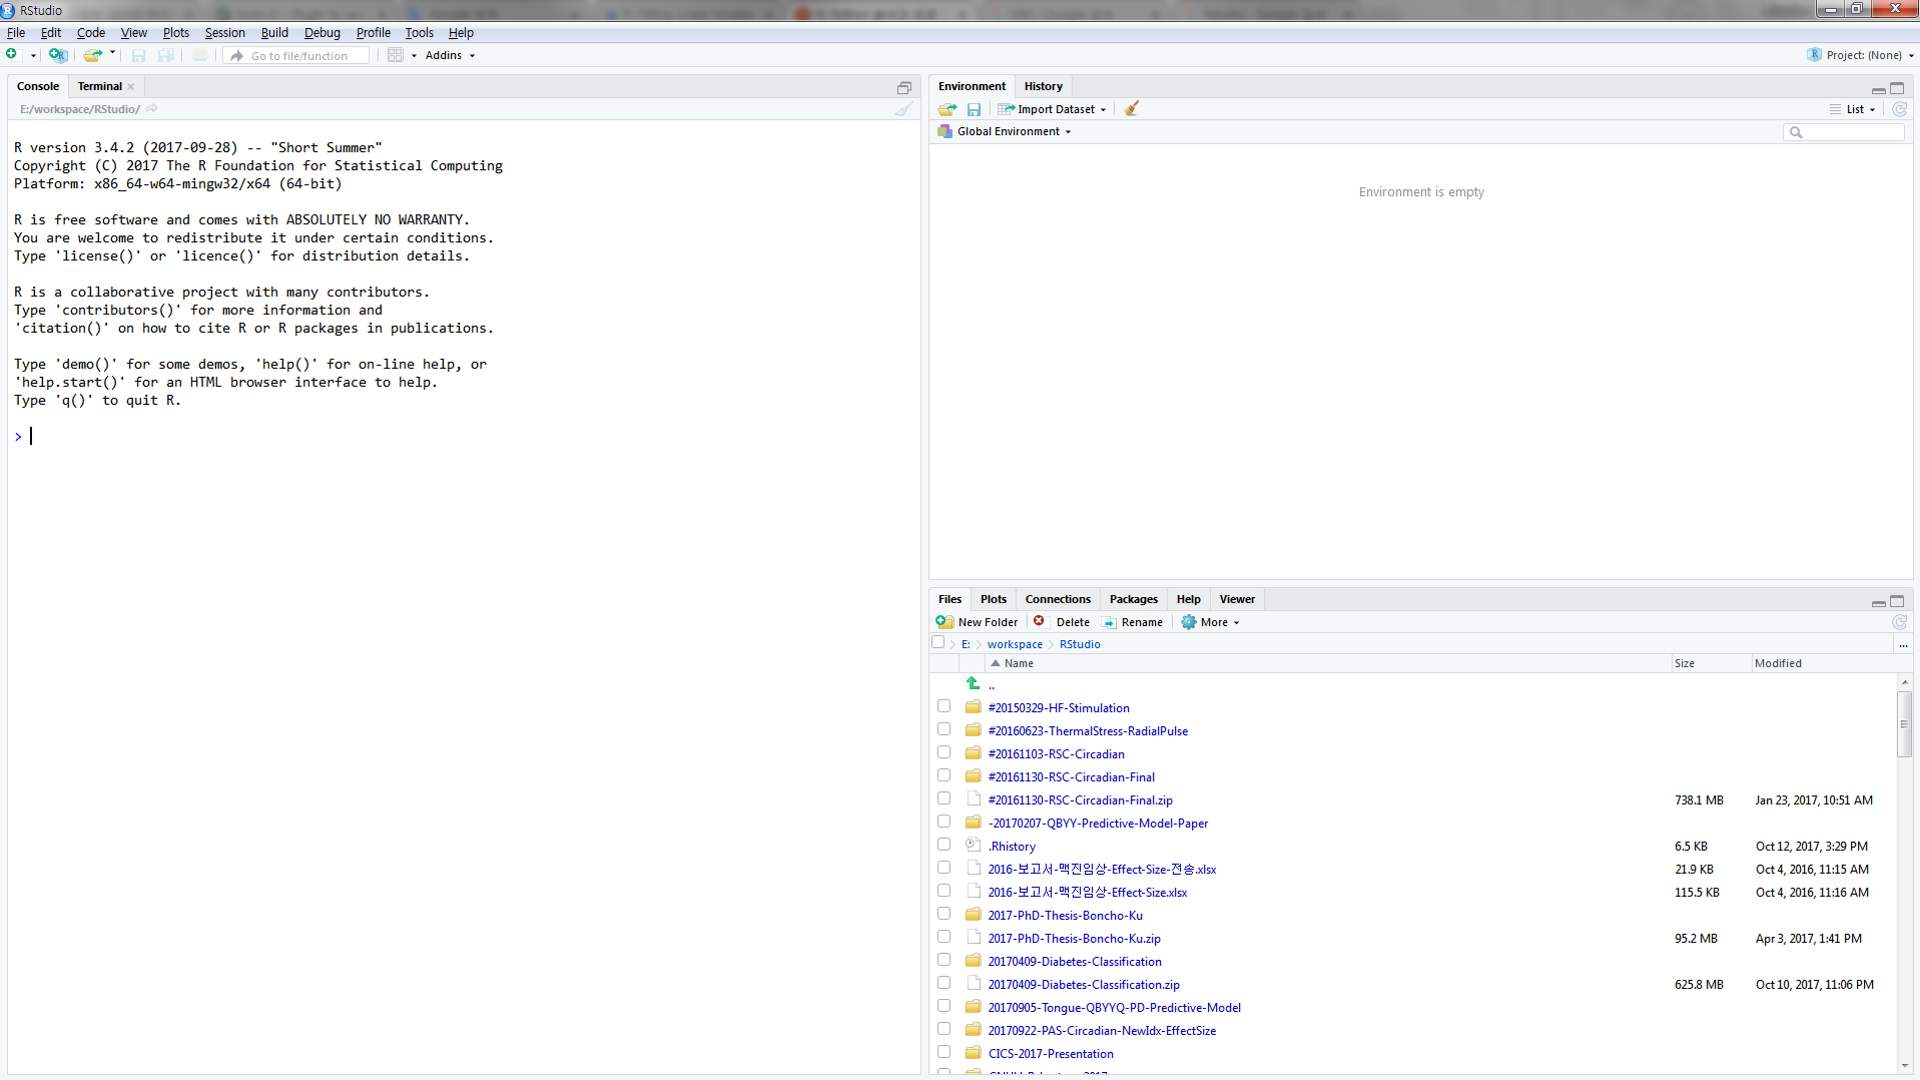
\includegraphics[width = 15cm, height = 13cm]{Figures/Rstudio-init.png}
  \caption[RStudio 초기 실행화면]{RStudio 초기 실행화면}\label{fig:Rstudio-install-05}
}
\end{figure}

\section{RStudio의 구성}\label{rstudio-}

\subsection{RStudio IDE 화면 구성}\label{rstudio-ide--}

RStudio는 아래 그림 \ref{fig:Rstudio-part-01}과 같이 크게 4개 창으로
구성

\begin{figure}[H]
{
  \centering
  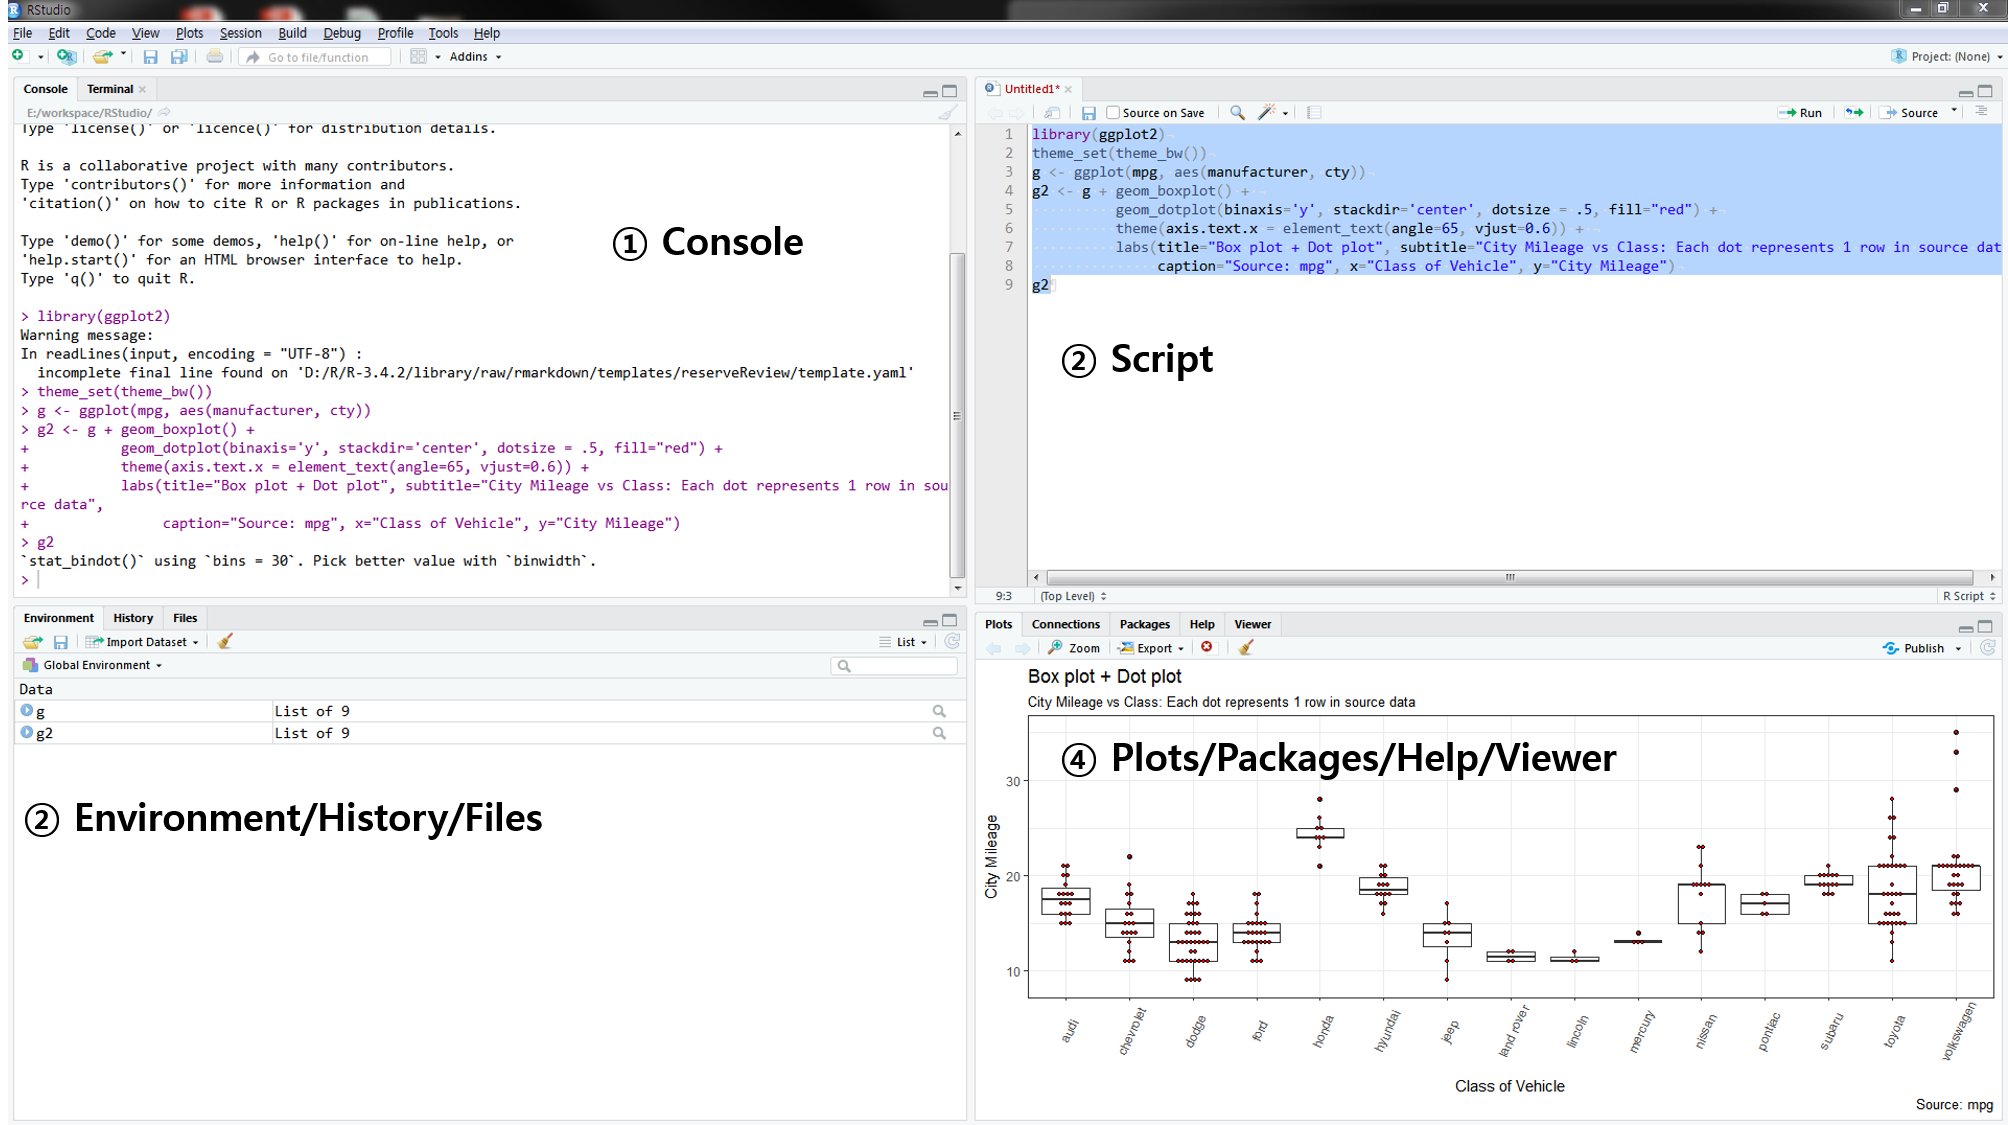
\includegraphics[width = 14cm, height = 12cm]{Figures/Rstudio-cap1.png}
  \caption[RStudio 화면구성]{RStudio 화면구성: 우하단 그림은 http://r-statistics.co/Top50-Ggplot2-Visualizations-MasterList-R-Code.html 에서 발췌}\label{fig:Rstudio-part-01}
}
\end{figure}

\begin{enumerate}
\def\labelenumi{\arabic{enumi}.}
\tightlist
\item
  콘솔(console)

  \begin{itemize}
  \tightlist
  \item
    R 명령어 실행 공간(RGui, 정확하게는 \texttt{Rterm.exe}가 실행되고
    있는 창)
  \item
    R 스크립트 또는 콘솔 창에서 작성한 명령어(프로그램) 실행 결과 출력
  \item
    경고, 에러/로그 등의 메세지 확인
  \end{itemize}
\item
  스크립트(script) R 명령어 입력 공간으로 일괄처리(batch processing)
  가능

  \begin{itemize}
  \tightlist
  \item
    일괄 처리를 위한 RStudio 제공 단축키

    \begin{itemize}
    \tightlist
    \item
      \keystroke{Ctrl} + \keystroke{Enter}: 선택한 블럭 내 명령어 실행
    \item
      \keystroke{Alt} + \keystroke{Enter}: 선택 없이 커서가 위치한
      라인의 명령어 실행
    \end{itemize}
  \item
    새 R 스크립트 파일 열기

    \begin{itemize}
    \tightlist
    \item
      R 상단 메뉴: \texttt{{[}File{]}} \(\rightarrow\)
      \texttt{{[}New\ File{]}} \(\rightarrow\) \texttt{{[}R\ Script{]}}
    \item
      단축키: \keystroke{Ctrl} + \keystroke{Shift} + \keystroke{N}
    \end{itemize}
  \item
    R 스크립트 이외 \texttt{R\ Markdown}, \texttt{R\ Notebook},
    \texttt{Shiny\ Web\ Application} 등 새 문서의 목적에 따라 다양한
    종류의 문서 생성 가능
  \end{itemize}
\item
  Environment/History

  \begin{enumerate}
  \def\labelenumii{\arabic{enumii})}
  \tightlist
  \item
    Environment: 현재 R 작업환경에 저장되어 있는 객체의 특성을 요약 제시

    \begin{itemize}
    \tightlist
    \item
      좌측 화살표 버튼 클릭: 해당 객체의 상세 정보 확인(그림
      \ref{fig:Rstudio-envirn-01})
    \item
      우측 사각형 버튼 클릭: 객체가 데이터프레임인 경우 스프레드 시트
      형태로 데이터셋 확인(그림 \ref{fig:Rstudio-envirn-02})
    \item
      디스켓 아이콘: 작업공간 저장 여부
    \item
      빗자루 아이콘: 작업공간 객체 일괄 삭제
    \item
      Global Environment 아이콘: 현재 작업공간에서 사용중인 패키지 및
      선택 패키지 내장 함수 목록 확인

      \begin{figure}[H] {
        \centering
        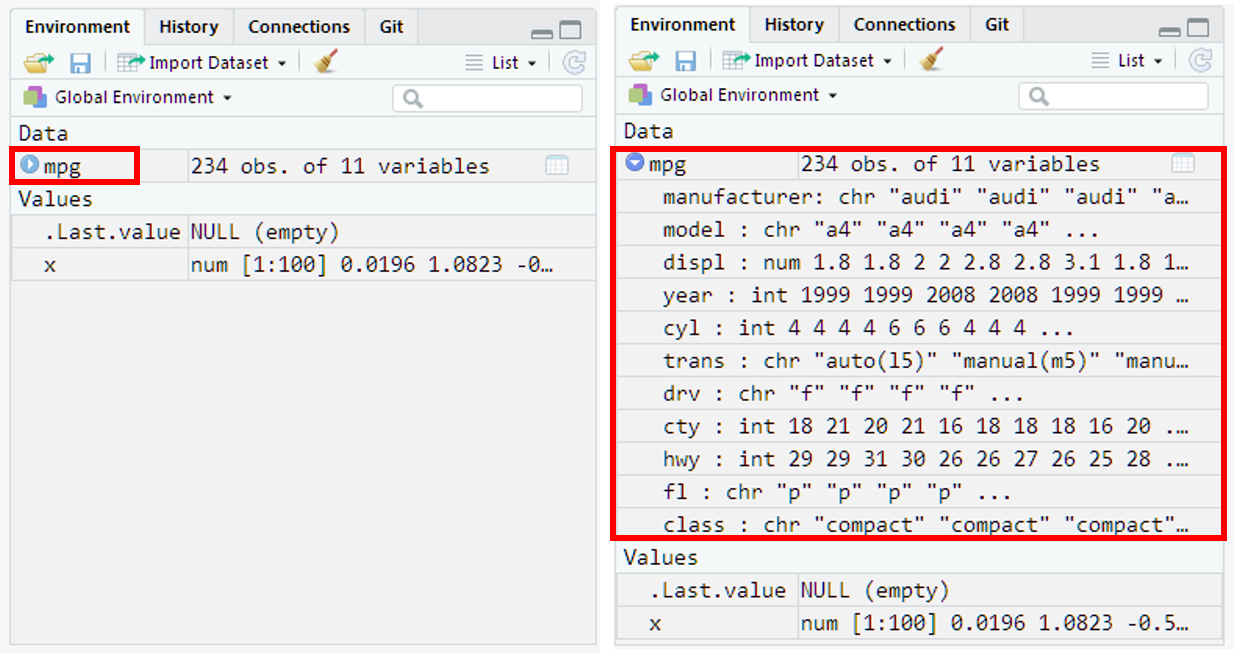
\includegraphics[width = 12cm, height = 10cm]{Figures/Rstudio-envwin-01.png}
        \caption[RStudio Environment 창: 객체 상세정보]{RStudio Environment 창: 객체 상세정보}\label{fig:Rstudio-envirn-01}
      } \end{figure}\begin{figure}[H] {
        \centering
        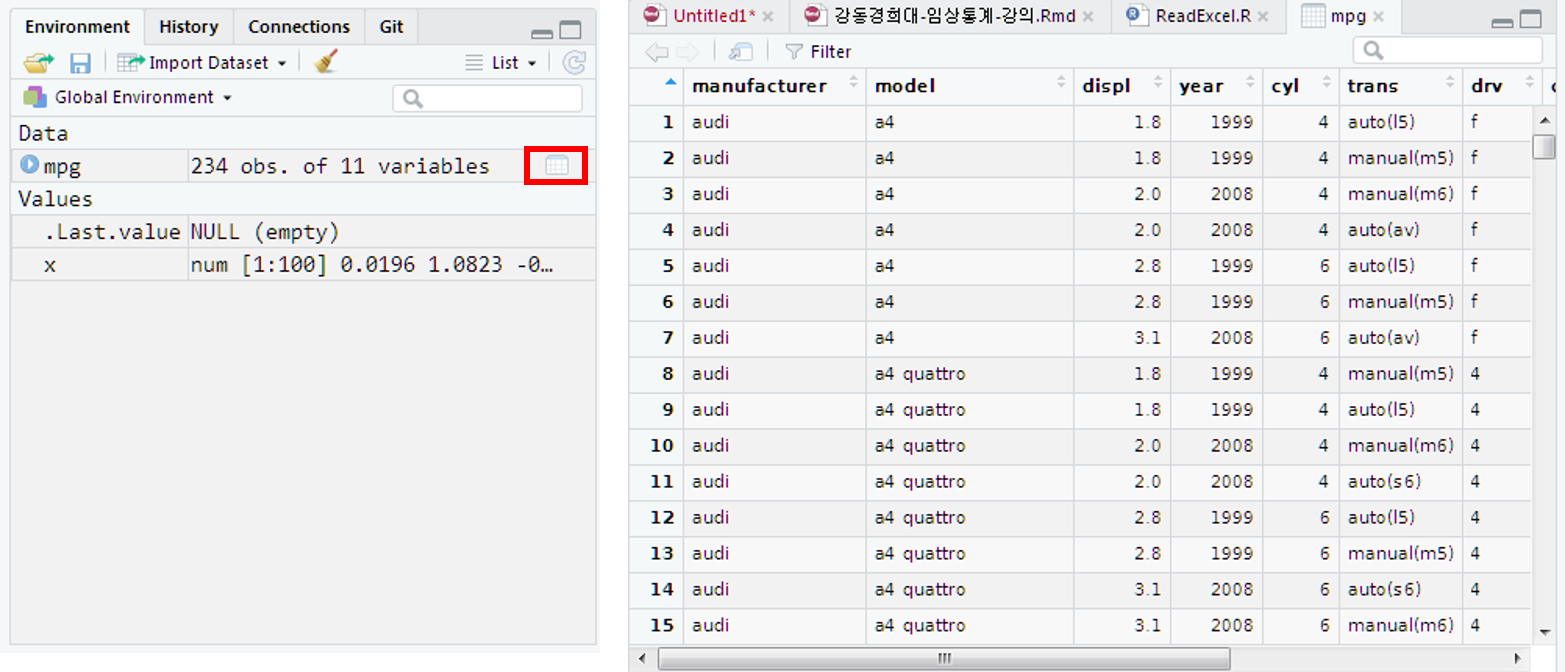
\includegraphics[width = 15cm, height = 10cm]{Figures/Rstudio-envwin-02.png}
        \caption[RStudio Environment 창: 스프레드 시트]{RStudio Environment 창: 스프레드 시트}\label{fig:Rstudio-envirn-02}
      } \end{figure}
    \item
      History: R 콘솔에서 실행된 명령어(스크립트)들의 이력 확인

      \begin{figure}[H] {
        \centering
        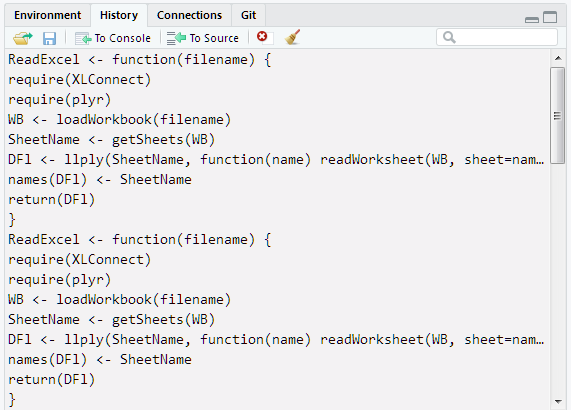
\includegraphics[width = 8cm, height = 8cm]{Figures/Rstudio-historywin.png}
        \caption[RStudio History 창]{RStudio History 창}\label{fig:Rstudio-history}
      } \end{figure}
    \end{itemize}
  \end{enumerate}
\item
  File/Plots/Packages/Help/Viewer

  \begin{enumerate}
  \def\labelenumii{\arabic{enumii})}
  \tightlist
  \item
    File: Windows 탐색기와 유사

    \begin{itemize}
    \tightlist
    \item
      파일 및 폴더 생성, 삭제 수정, 그리고 작업경로 설정

      \begin{figure}[H] {
        \centering
        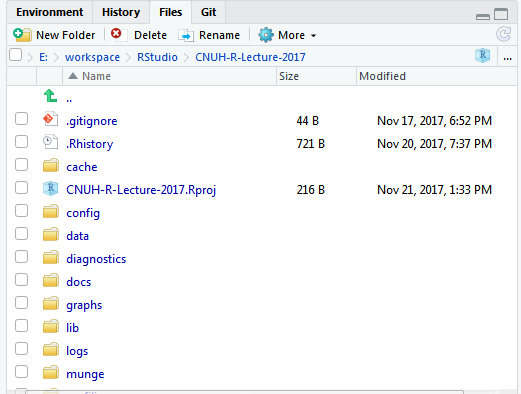
\includegraphics[width = 8cm, height = 8cm]{Figures/Rstudio-file.png}
        \caption[RStudio File 창]{RStudio File 창}\label{fig:Rstudio-file}
      } \end{figure}
    \end{itemize}
  \item
    Plots: 콘솔 또는 스크립트 창으로부터 생성한 그래프 출력

    \begin{itemize}
    \tightlist
    \item
      작업 중 생성한 그래프가 이력에 따라 저장: \keystroke{$\Leftarrow$}
      이전, \keystroke{$\Rightarrow$} 최근
    \item
      \keystroke{Zoom} 기능으로 그래프 확대 가능
    \item
      \keystroke{Export}를 통해 선택 그래프를 이미지 파일(\texttt{.png},
      \texttt{.jpeg} 등), PDF 파일 및 PDF 출력 파일로 저장 가능
    \item
      엑스박스는 현재 화면에 출력된 그래프 삭제, 빗자루 아이콘은 생성한
      모든 그래프 삭제

      \begin{figure}[H] {
        \centering
        \includegraphics[width = 8cm, height = 8cm]{Figures/Rstudio-plotwin.png}
        \caption[RStudio Plots 창 화면]{RStudio Plots 창 화면}\label{fig:Rstudio-plot}
      } \end{figure}
    \end{itemize}
  \item
    Packages: 현재 컴퓨터에 설치된 R 패키지 목록 출력: 신규 설치 및
    업데이트 가능

    \begin{figure}[H] {
      \centering
      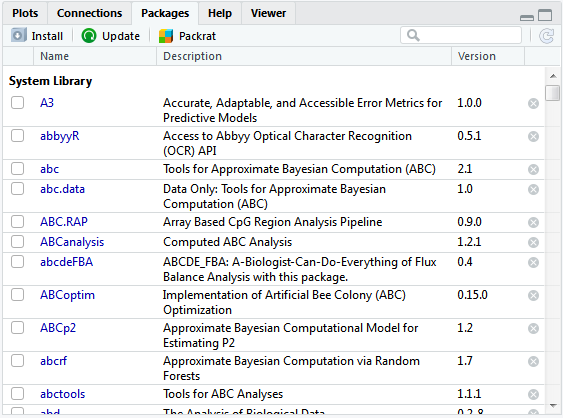
\includegraphics[width = 8cm, height = 8cm]{Figures/RStudio-packagewin.png}
      \caption[RStudio Packages 창 화면]{RStudio Packages 창 화면}\label{fig:Rstudio-pkgwin}
    } \end{figure}
  \item
    Help: \texttt{help(topic)} 입력 시 도움말 창이 출력되는 공간
    \footnotesize
  \end{enumerate}
\end{enumerate}

\begin{Shaded}
\begin{Highlighting}[]
\OperatorTok{>}\StringTok{ }\KeywordTok{help}\NormalTok{(lm)}
\end{Highlighting}
\end{Shaded}

\normalsize

\begin{figure}[H] {
  \centering
  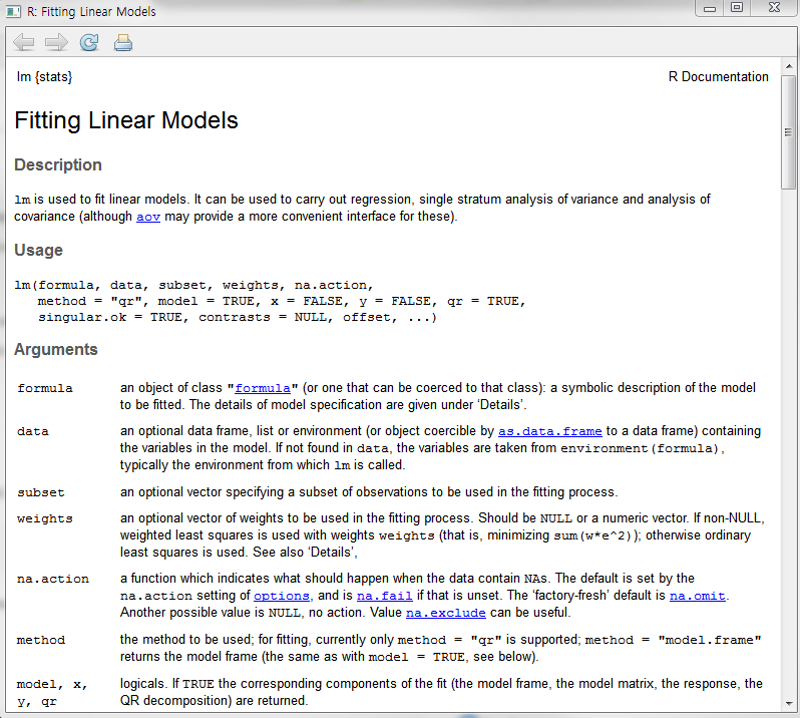
\includegraphics[width = 8cm, height = 8cm]{Figures/RStudio-helpwin.png}
  \caption[\texttt{help(lm)} 실행 후 RStudio Help 창 화면]{\texttt{help(lm)} 실행 후 RStudio Help 창 화면}\label{fig:Rstudio-hlpwin}
} \end{figure}

\begin{enumerate}
\def\labelenumi{\arabic{enumi}.}
\setcounter{enumi}{4}
\tightlist
\item
  RStudio의 창 layout은 \texttt{{[}Tools{]}} \(\rightarrow\)
  \texttt{{[}Global\ Options{]}} \(\rightarrow\)
  \texttt{{[}Pane\ Layout{]}}에서 변경 가능
\end{enumerate}

\begin{figure}[H] {
  \centering
  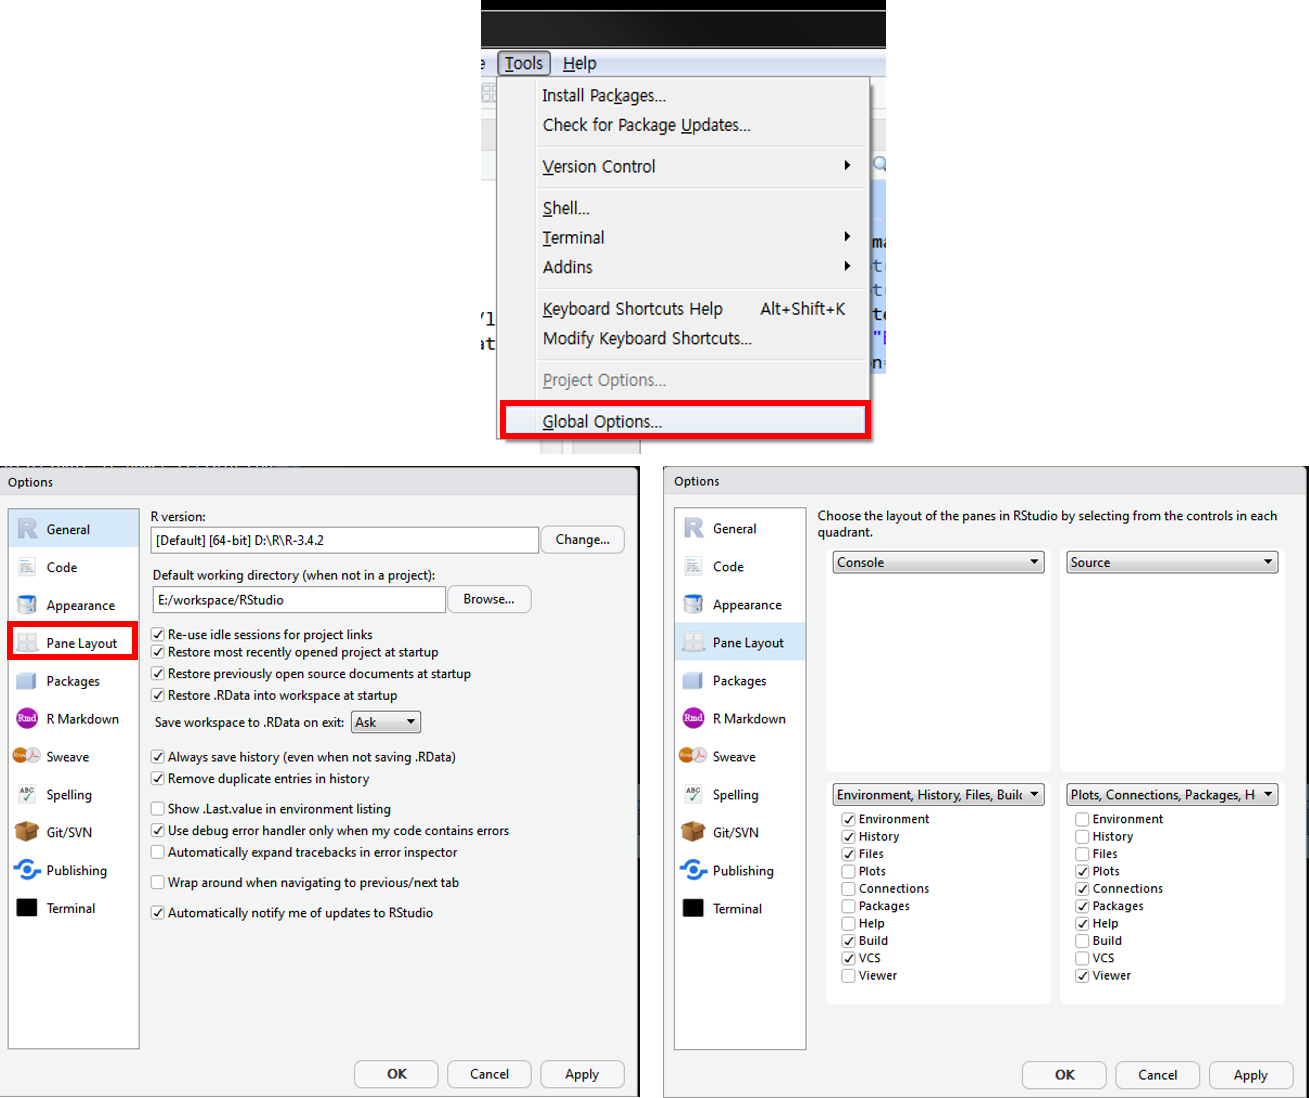
\includegraphics[width = 15cm, height = 10cm]{Figures/RStudio-layout.png}
  \caption[RStudio Option 선택화면 및 Pane 레이아웃 선택 화면]{RStudio Option 선택화면 및 Pane 레이아웃 선택 화면}\label{fig:Rstudio-layout}
} \end{figure}

\section{RStudio에서 배치 파일 생성 및 실행}\label{rstudio-----}

스크립트 파일 생성, 저장, 실행

\begin{enumerate}
\def\labelenumi{\arabic{enumi}.}
\tightlist
\item
  R 소스 파일 실행

  \begin{itemize}
  \tightlist
  \item
    \keystroke{Ctrl} + \keystroke{Shift} + \keystroke{S}
  \item
    \keystroke{Ctrl} + \keystroke{Shift} + \keystroke{Enter}
  \item
    \texttt{source("파일이름")}
  \end{itemize}
\item
  파일 경로 설정

  \begin{itemize}
  \tightlist
  \item
    R에서 디렉토리 구분자는 \texttt{/}임
  \item
    Windows에서 사용하는 \texttt{\textbackslash{}}는 특수문자로 간주
  \item
    경로 복사 후 R에서 사용하는 경우 \texttt{\textbackslash{}}를
    \texttt{\textbackslash{}\textbackslash{}}로 변경해야 인식
  \end{itemize}
\end{enumerate}

\section{R 패키지 설치}\label{r--}

\begin{enumerate}
\def\labelenumi{\arabic{enumi}.}
\tightlist
\item
  RStudio 메뉴 \texttt{{[}Tools{]}} \(\rightarrow\)
  \texttt{{[}Install\ packages{]}} 클릭 후 생성된 팝업 창에서 설치하고자
  하는 패키지 입력 후 설치
\item
  RStudio \texttt{Packages} 창에서 \keystroke{Install} 버튼 누르고
  설치(위와 동일)
\item
  R 콘솔 또는 스크립트 창에서 \texttt{install.packages()}
\end{enumerate}

\subsection{패키지 불러오기}\label{-}

\begin{enumerate}
\def\labelenumi{\arabic{enumi}.}
\tightlist
\item
  \texttt{library()} vs. \texttt{require()}

  \begin{itemize}
  \tightlist
  \item
    \texttt{library()}: 불러오고자 하는 패키지가 시스템에 존재하지 않는
    경우 에러 메세지 출력(에러 이후 명령어들이 실행되지 않음)
  \item
    \texttt{require()}: 패키지가 시스템에 존재하지 않는 경우 경고 메세지
    출력(경고 이후 명령어 정상적으로 실행)
  \end{itemize}
\item
  다중 패키지 동시에 불러오기

  \begin{itemize}
  \tightlist
  \item
    RStudio \texttt{Packages} 창에서 설치하고자 하는 패키지 선택 버튼
    클릭하면 R workspace로 해당 패키지 로드 가능
  \item
    스크립트 이용
  \end{itemize}
\end{enumerate}

\footnotesize

\begin{Shaded}
\begin{Highlighting}[]
\NormalTok{pkgName <-}\StringTok{ }\KeywordTok{c}\NormalTok{(}\StringTok{"MASS"}\NormalTok{, }\StringTok{"tidyverse"}\NormalTok{, }\StringTok{"ggthemes"}\NormalTok{, }\StringTok{"readxl"}\NormalTok{, }\StringTok{"ProjectTemplate"}\NormalTok{, }\StringTok{"kableExtra"}\NormalTok{, }
    \StringTok{"ztable"}\NormalTok{, }\StringTok{"car"}\NormalTok{, }\StringTok{"lsmeans"}\NormalTok{)}
\CommentTok{# 'lapply()': 벡터, 리스트 또는 표현식에 함수를 적용하여 그 결과를 리스트로 반환}
\KeywordTok{lapply}\NormalTok{(pkgName, require, }\DataTypeTok{character.only =}\NormalTok{ T)}
\end{Highlighting}
\end{Shaded}

\normalsize

\section{\texorpdfstring{\texttt{rJava}
설치하기}{rJava 설치하기}}\label{rjava-}

\begin{enumerate}
\def\labelenumi{\arabic{enumi}.}
\item
  자바 명령을 호출하는 패키지를 정상적으로 사용하기 위한 패키지

  \begin{itemize}
  \tightlist
  \item
    Java 계열 머신러닝 어플리케이션 활용 또는 최근까지 Excel 파일을
    불러오기 위해 설치 필수(Excel에 관해서는 Hadley Wickham의
    \texttt{readxl} 개발 이전에는\ldots{})
  \item
    다음은 Java가 설치되지 않은 환경에서 \texttt{rJava}를 불렀을 때
    발생한 오류 예시임

    \begin{figure}[H] {
      \centering
      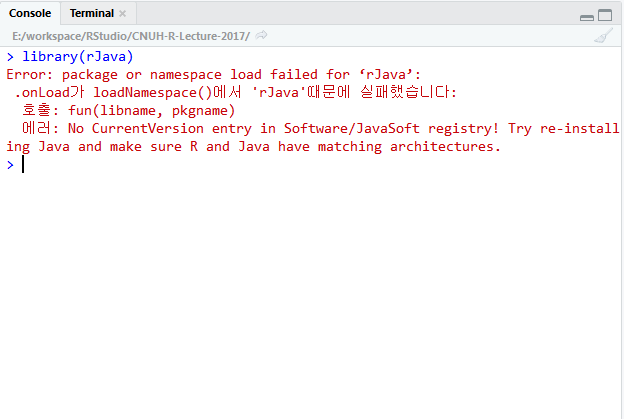
\includegraphics[width = 10cm, height = 8cm]{Figures/R-rJava-error.png}
      \caption[\texttt{rJava} 에러 메세지]{\texttt{rJava} 에러 메세지}\label{fig:rJava-error}
    } \end{figure}
  \end{itemize}
\item
  \texttt{rJava} 설치 전 자바 설치 및 Windows 시스템 환경 설정 필요
\item
  자바 개발 키트(Java Development Kit, JDK)는
  \url{http://www.oracle.com/technetwork/java/javase/downloads/index.html}
  에서 다운로드 가능

  \begin{itemize}
  \tightlist
  \item
    \texttt{{[}Java\ Platform\ (JDK){]}} \(\rightarrow\)
    \texttt{{[}Download{]}} 클릭

    \begin{figure}[H] {
      \centering
      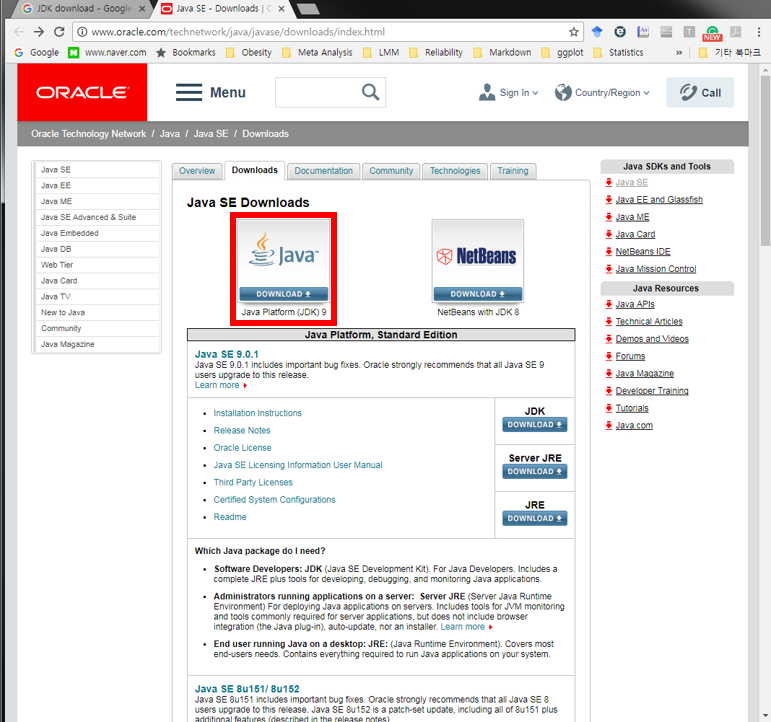
\includegraphics[width = 10cm, height = 10cm]{Figures/R-rJava-install-01.png}
      \caption[JDK 다운로드 메인 페이지]{JDK 다운로드 페이지}\label{fig:rJava-01}
    } \end{figure}
  \end{itemize}
\item
  JDK 다운로드 전 현재 주로 작업하고 있는 R 버전 정보(32 bit vs.~64 bit)
  확인

  \begin{itemize}
  \tightlist
  \item
    R 세션 시작 시 또는 RStudio에서 \texttt{{[}Tools{]}} \(\rightarrow\)
    \texttt{{[}Global\ Options{]}}에서 R 버전 확인 가능
  \item
    라이센스 계약에 동의 후 확인한 R 버전에 대응하는 링크 클릭 후
    다운로드 진행

    \begin{figure}[H] {
      \centering
      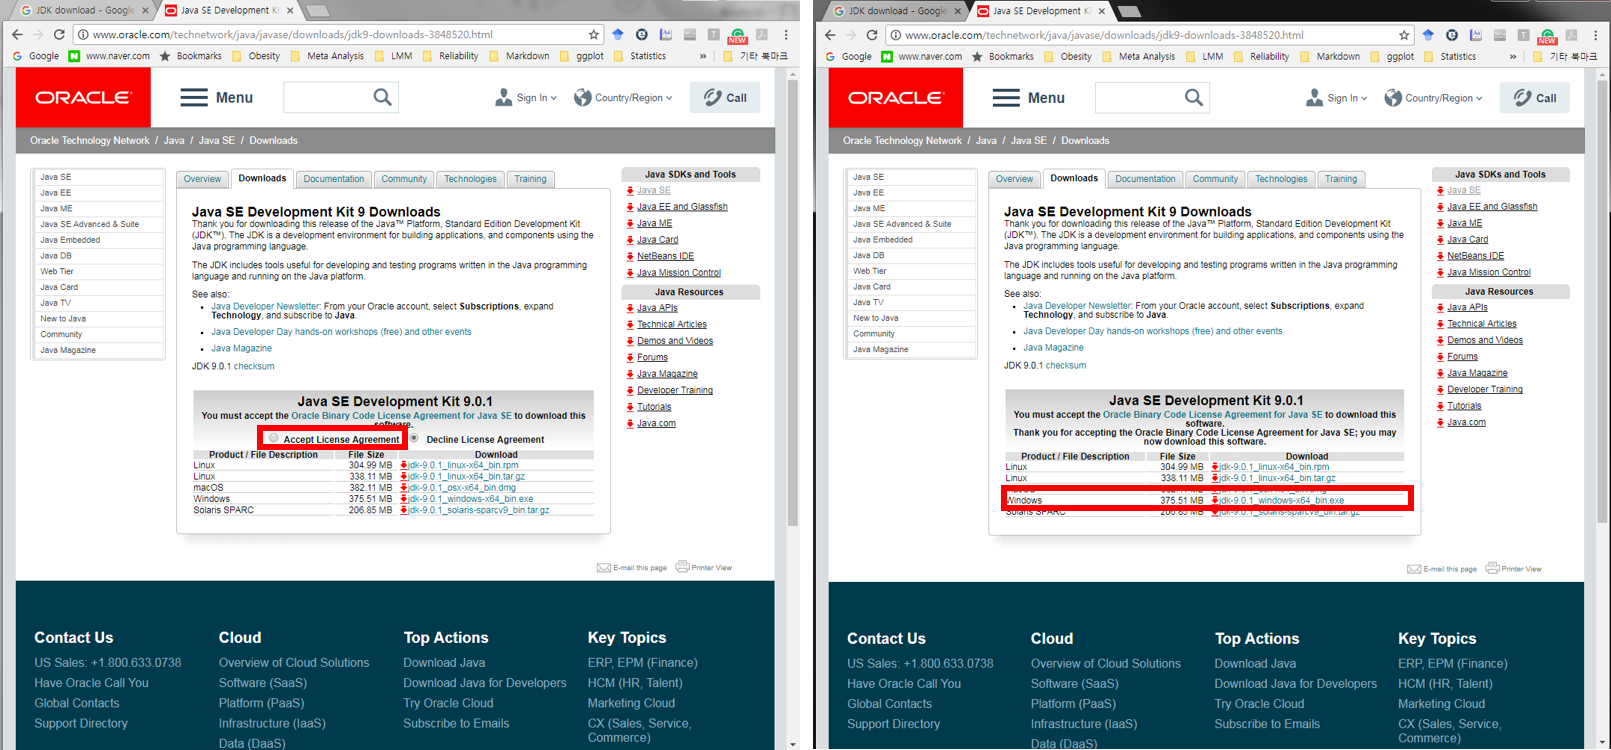
\includegraphics[width = 15cm, height = 10cm]{Figures/R-rJava-install-02.png}
      \caption[JDK 라이센스 및 다운로드 링크 페이지]{JDK 라이센스 및 다운로드 링크 페이지}\label{fig:rJava-02}
    } \end{figure}
  \end{itemize}
\item
  다운로드 완료 후 설치 확인

  \begin{itemize}
  \tightlist
  \item
    정상적으로 설치한 경우라면
    \texttt{C:\textbackslash{}Program\ Files\textbackslash{}Java\textbackslash{}jdk-9.0.1}
    디렉토리에서 설치 확인 가능
  \item
    Java runtime environment (JRE)는
    \texttt{C:\textbackslash{}Program\ Files\textbackslash{}Java\textbackslash{}jre-9.0.1}
    에서 설치 확인 가능
  \end{itemize}
\item
  새 사용자 변수 생성

  \begin{itemize}
  \tightlist
  \item
    \keystroke{Windows 시작} 클릭 \(\rightarrow\) \texttt{{[}컴퓨터{]}}
    우 클릭 \(\rightarrow\) \texttt{{[}속성{]}} 클릭 후 다음 그림
    \ref{fig:rJava-03}에서 \texttt{{[}고급\ 시스템\ 설정{]}} 클릭

    \begin{figure}[H] {
      \centering
      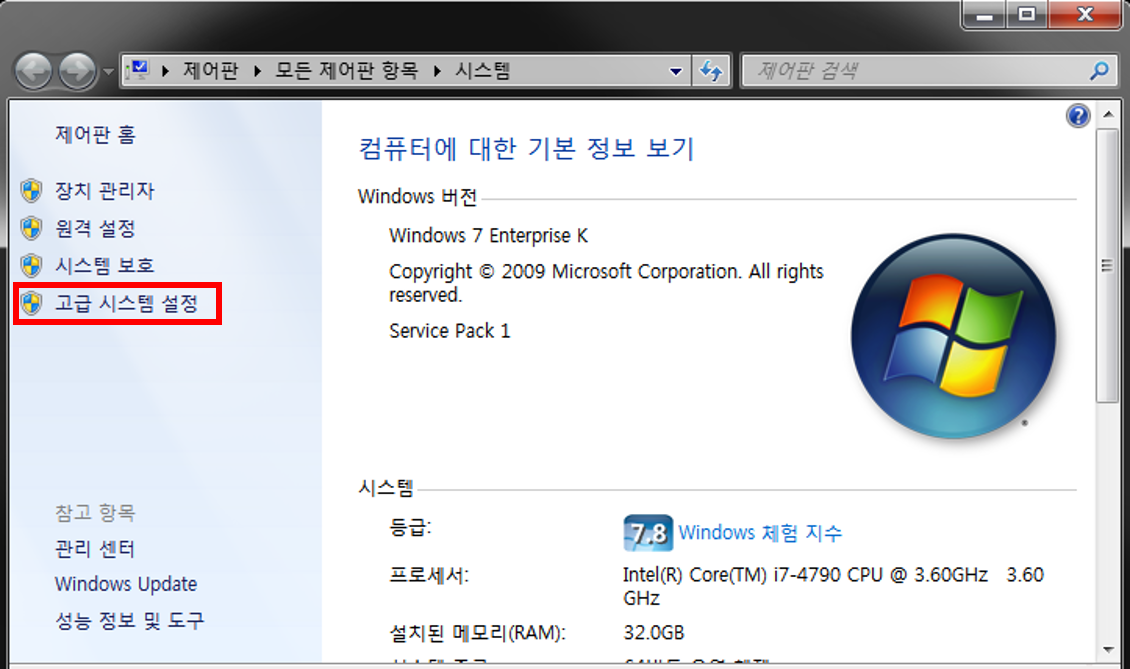
\includegraphics[width = 15cm, height = 10cm]{Figures/R-rJava-system.png}
      \caption[Windows 시스템 설정 화면]{Windows 시스템 설정 화면}\label{fig:rJava-03}
    } \end{figure}
  \item
    시스템 속성 창에서 \texttt{{[}환경변수(N)...{]}} 클릭 후 환경변수
    창에서 사용자 변수 \texttt{{[}새로\ 만들기(N)...{]}} 클릭
  \item
    변수 이름에 \texttt{JAVA\_HOME}, 변수 값에 JDK 설치 디렉토리
    이름(예:
    \texttt{C:\textbackslash{}Program\ Files\textbackslash{}Java\textbackslash{}jdk-9.0.1})
    입력

    \begin{figure}[H] {
      \centering
      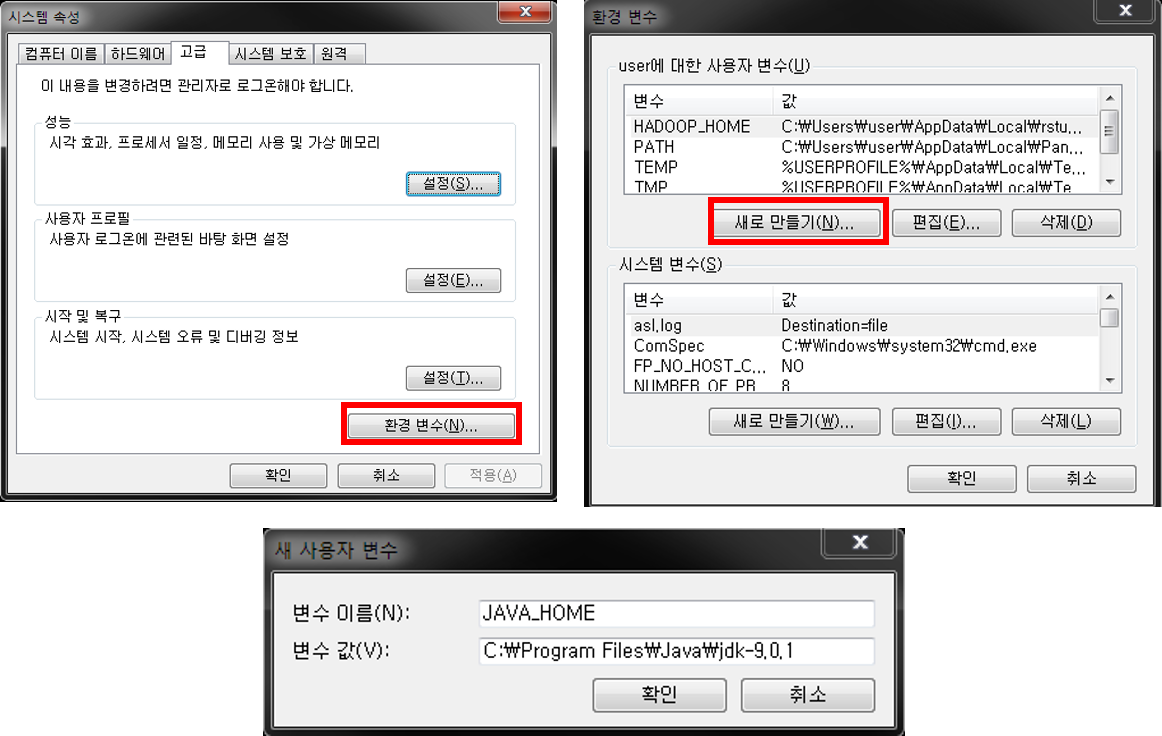
\includegraphics[width = 15cm, height = 10cm]{Figures/R-rJava-install-03.png}
      \caption[Windows 시스템 설정 화면]{Windows 시스템 설정 화면}\label{fig:rJava-04}
    } \end{figure}
  \end{itemize}
\item
  시스템 변수 \texttt{PATH} 갱신

  \begin{itemize}
  \tightlist
  \item
    JRE가 설치된 디렉토리(아래 나열)를 기존 \texttt{PATH}에
    추가(디렉토리 구분자: \texttt{;})

    \begin{itemize}
    \tightlist
    \item
      \texttt{C:\textbackslash{}Program\ Files\textbackslash{}Java\textbackslash{}jre-9.0.1\textbackslash{}bin}
    \item
      \texttt{C:\textbackslash{}Program\ Files\textbackslash{}Java\textbackslash{}jre-9.0.1\textbackslash{}bin\textbackslash{}server}
    \end{itemize}
  \end{itemize}
\item
  설정 완료 후 R 또는 RStudio 재실행 후 \texttt{rJava} 설치
\item
  별 다른 에러 메세지 출력이 없으면 성공적으로 설치
\end{enumerate}

\section{\texorpdfstring{RStudio 프로젝트 생성 및
\texttt{ProjectTemplate} 패키지
연동}{RStudio 프로젝트 생성 및 ProjectTemplate 패키지 연동}}\label{rstudio----projecttemplate--}

\subsection{RStudio 프로젝트}\label{rstudio-}

\begin{enumerate}
\def\labelenumi{\arabic{enumi}.}
\tightlist
\item
  프로젝트

  \begin{itemize}
  \tightlist
  \item
    물리적 측면: 최종 산출물(문서)를 생성하기 위한 데이터, 사진, 그림
    등을 모아 놓은 폴더
  \item
    논리적 측면: R 세션 및 작업의 버전 관리
  \end{itemize}
\item
  프로젝트의 필요성

  \begin{itemize}
  \tightlist
  \item
    자료의 정합성 보장
  \item
    다양한 확장자를 갖는 한 폴더 내에 뒤섞일 때 곤란해 질 수 있음
  \item
    실제 분석 및 그래프 생성에 사용한 정확한 프로그램 또는 코드 연결이
    어려움
  \end{itemize}
\item
  좋은 프로젝트 구성을 위한 방법

  \begin{itemize}
  \tightlist
  \item
    원자료(raw data)의 보호: 가급적 자료를 읽기 전용(read only) 형태로
    다루기
  \item
    데이터 정제(data wrangling 또는 data munging)를 위한 스크립트와 정제
    자료를 보관하는 읽기 전용 데이터 디렉토리 생성
  \item
    작성한 스크립트로 생성한 모든 산출물(테이블, 그래프 등)을
    ``일회용품''처럼 처리 \(\rightarrow\) 스크립트로 재현 가능
  \item
    한 프로젝트 내 각기 다른 분석마다 다른 하위 디렉토리에 출력결과
    저장하는 것이 유용
  \end{itemize}
\item
  RStudio 새로운 프로젝트 생성

  \begin{itemize}
  \tightlist
  \item
    RStudio의 가장 강력하고 유용한 기능
  \item
    새로운 프로젝트 생성

    \begin{enumerate}
    \def\labelenumii{\arabic{enumii})}
    \tightlist
    \item
      RStudio 메뉴에서 \texttt{{[}File{]}} \(\rightarrow\)
      \texttt{{[}New\ Project{]}} 선택하면 아래와 같은 팝업 메뉴 생성

      \begin{figure}[H] {
        \centering 
        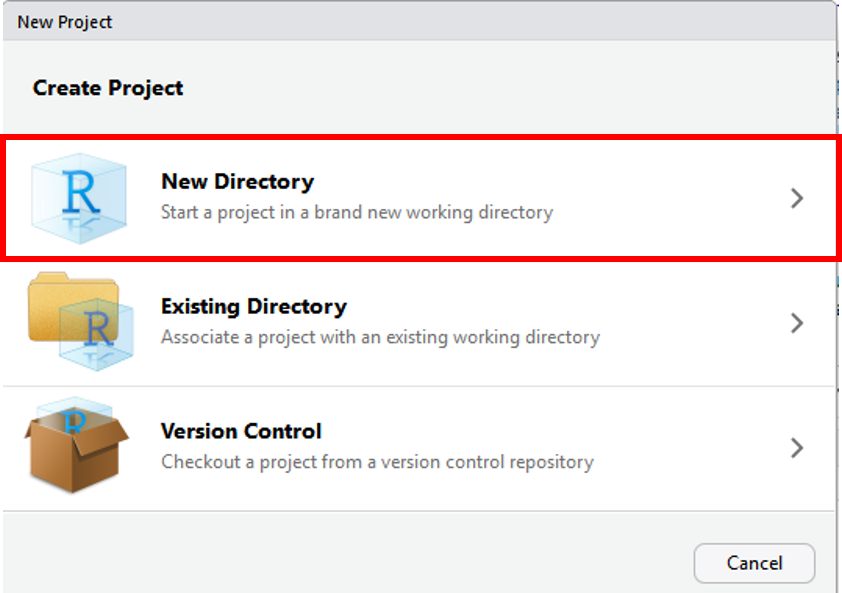
\includegraphics[width = 10cm, height = 10cm]{Figures/R-newproject-01.png}
        \caption[RStudio 새로운 프로젝트 생성]{RStudio 새로운 프로젝트 생성}\label{fig:RStudio-project-01}
      } \end{figure}

      \begin{itemize}
      \tightlist
      \item
        \keystroke{Existing Directory}: 이미 작업공간이 존재하고 있는
        경우 해당 디렉토리 선택(다루지 않음)
      \item
        \keystroke{Version Control}: 버전관리 시스템(Git, SVN)의
        저장소에 존재하는 프로젝트 작업 시 선택(다루지 않음)
      \end{itemize}
    \item
      그림 \ref{fig:RStudio-project-01}에서 \keystroke{New Directory}
      선택 후 다음 창으로 이동

      \begin{figure}[H] {
        \centering 
        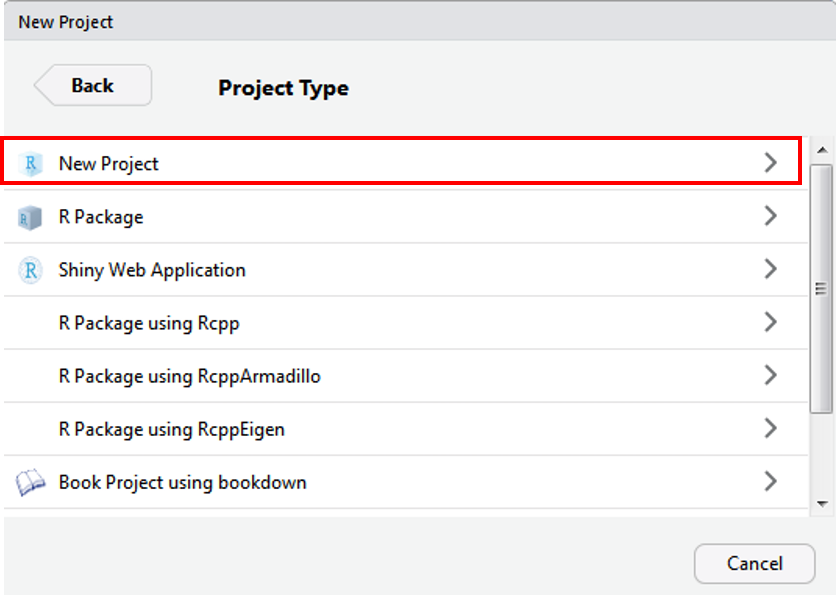
\includegraphics[width = 8cm, height = 8cm]{Figures/R-newproject-02.png}
        \caption[RStudio 새로운 프로젝트 유형 선택]{RStudio 새로운 프로젝트 유형 선택}\label{fig:RStudio-project-02}
      } \end{figure}

      \begin{itemize}
      \tightlist
      \item
        \keystroke{New Project}: 자료분석을 위한 프로젝트 생성
      \item
        \keystroke{R Package}: 패키지 개발을 위한 작업 프로젝트 생성
      \item
        \keystroke{Shiny Web Application}: Shiny를 이용한 데이터 연동형
        웹 어플리케이션 개발 프로젝트 생성
      \item
        \keystroke{Book Project using bookdown}: 책 지필 작업을 위한
        프로젝트 생성
      \end{itemize}
    \item
      \keystroke{New Project} 선택 후 프로젝트 저장 폴더 생성 창으로
      이동

      \begin{figure}[H] {
        \centering 
        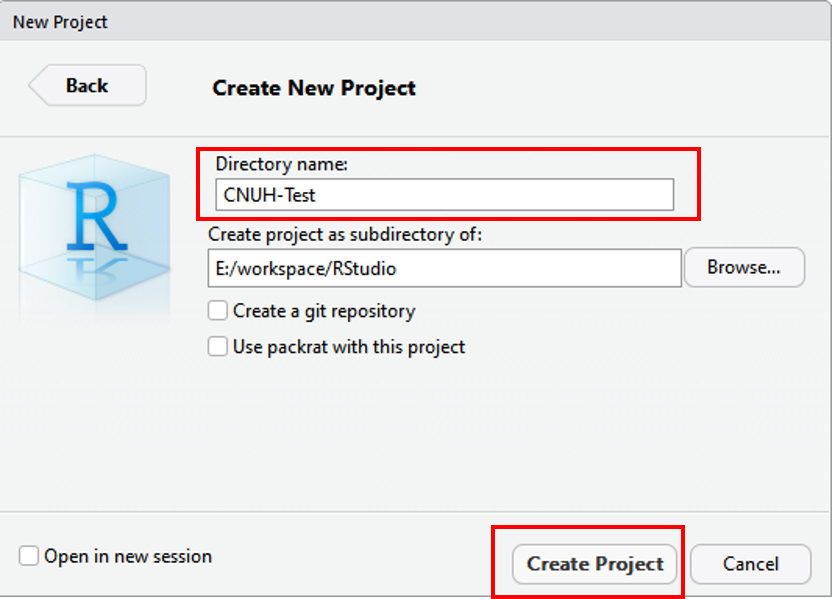
\includegraphics[width = 8cm, height = 8cm]{Figures/R-newproject-03.png}
        \caption[새로운 프로젝트의 폴더명 지정]{새로운 프로젝트의 폴더명 지정}\label{fig:RStudio-project-03}
      } \end{figure}

      \begin{itemize}
      \tightlist
      \item
        여기서는 \texttt{CNUH-Test}라는 프로젝트 이름으로 폴더 생성
      \item
        아래 \texttt{{[}Create\ projects\ as\ subdirectories\ of{]}}에서
        생성하고자 하는 프로젝트의 상위 디렉토리 설정 \(\rightarrow\)
        보통 RStudio의 default working directory로 기본 설정되어 있음.
      \item
        입력 완료 후 \keystroke{Create Project} 클릭 후 새로운 R 세션
        화면이 열리는 것을 확인 했으면 새로운 프로젝트 생성 완료
      \end{itemize}
    \item
      생성한 프로젝트 확인

      \begin{itemize}
      \tightlist
      \item
        새로운 R 세션 콘솔 창에 \texttt{getwd()}로 생성한 프로젝트 폴더
        확인
      \item
        아래 그림처럼 생성 프로젝트 폴더에 \texttt{CNUH-Test.RProj}
        실행파일 확인\\

        \begin{figure}[H] {
          \centering 
          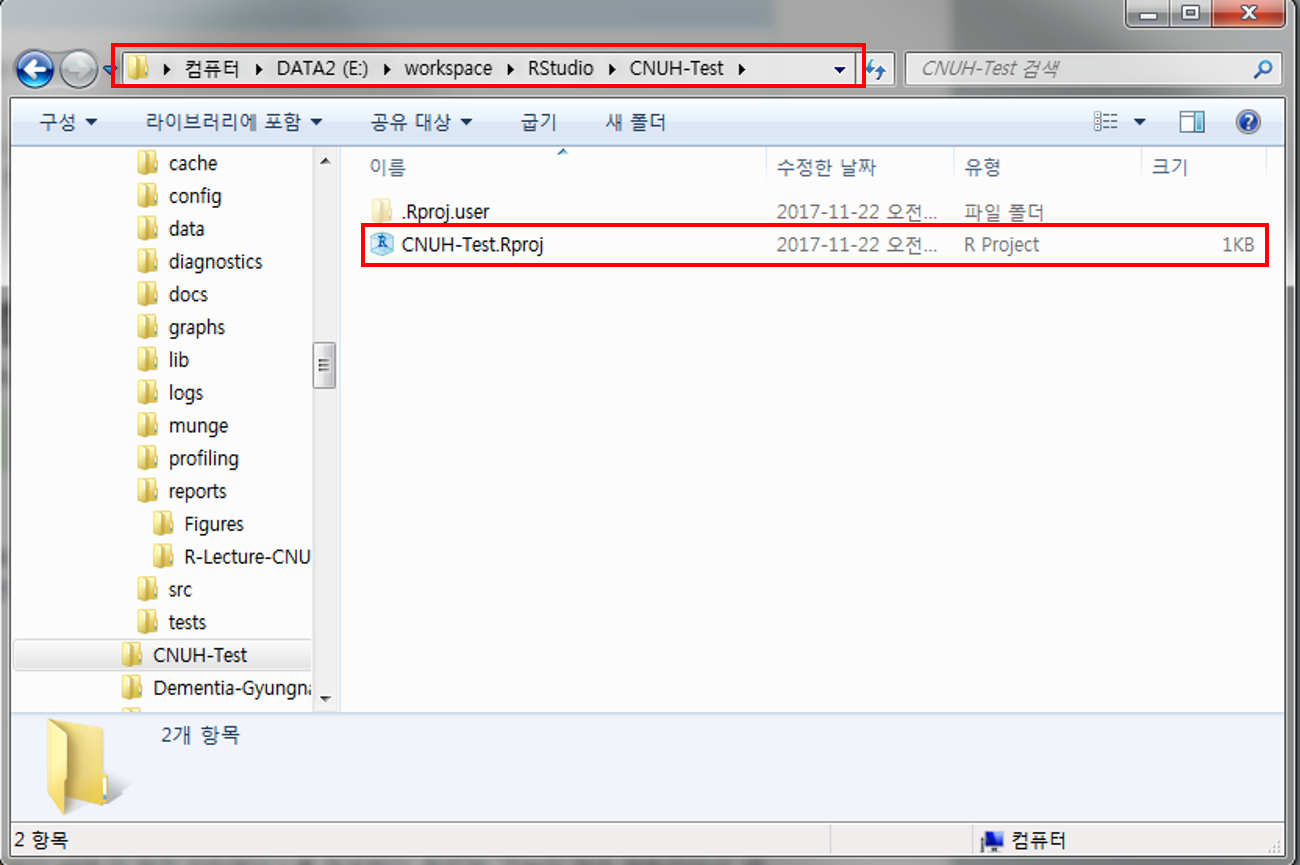
\includegraphics[width = 10cm, height = 8cm]{Figures/R-newproject-04.png}
          \caption[프로젝트 폴더 내 실행 파일 생성 확인]{프로젝트 폴더 내 실행 파일 생성 확인}\label{fig:RStudio-project-04}
        } \end{figure}
      \end{itemize}
    \end{enumerate}
  \end{itemize}
\end{enumerate}

\subsection{\texorpdfstring{\texttt{ProjectTemplate}}{ProjectTemplate}}\label{projecttemplate}

\begin{enumerate}
\def\labelenumi{\arabic{enumi}.}
\tightlist
\item
  프로젝트 관리를 자동화 하기 위한 솔루션을 제공하는 R 패키지

  \begin{itemize}
  \tightlist
  \item
    프로젝트 관리에 이상적인 directory 구조 제공
  \item
    자동으로 분석 파이프라인 및 작업흐름을 구성해서 구조화 함
  \item
    RStudio Project + \texttt{ProjectTemplate} + Git: 작업 기록 및 공동
    작업 가능
  \item
    \texttt{ProjectTemplate}의 자세한 사항은 다음 링크
    \url{http://projecttemplate.net/index.html} 참조
  \end{itemize}
\item
  \texttt{ProjectTemplate} 설치 및 생성
\end{enumerate}

\begin{enumerate}
\def\labelenumi{\arabic{enumi})}
\tightlist
\item
  \texttt{install.packages()} 함수를 이용해 설치
\end{enumerate}

\footnotesize

\begin{Shaded}
\begin{Highlighting}[]
\OperatorTok{>}\StringTok{ }\KeywordTok{install.packages}\NormalTok{(}\StringTok{"ProjectTemplate"}\NormalTok{)}
\end{Highlighting}
\end{Shaded}

\normalsize
 2) 패키지 불러오기

\footnotesize

\begin{Shaded}
\begin{Highlighting}[]
\OperatorTok{>}\StringTok{ }\KeywordTok{library}\NormalTok{(ProjectTemplate)}
\end{Highlighting}
\end{Shaded}

\normalsize
 3) \texttt{ProjectTemplate} 작업환경 생성 \footnotesize

\begin{Shaded}
\begin{Highlighting}[]
\OperatorTok{>}\StringTok{ }\CommentTok{# '..'는 default working directory 지시변수}
\ErrorTok{>}\StringTok{ }\KeywordTok{create.project}\NormalTok{(}\StringTok{"../CNUH-Test"}\NormalTok{, }\DataTypeTok{merge.strategy =} \StringTok{"allow.non.conflict"}\NormalTok{)}
\end{Highlighting}
\end{Shaded}

\normalsize

\begin{enumerate}
\def\labelenumi{\arabic{enumi})}
\setcounter{enumi}{3}
\tightlist
\item
  프로젝트 폴더 내 아래 폴더 생성 확인

  \begin{figure}[H] {
    \centering 
    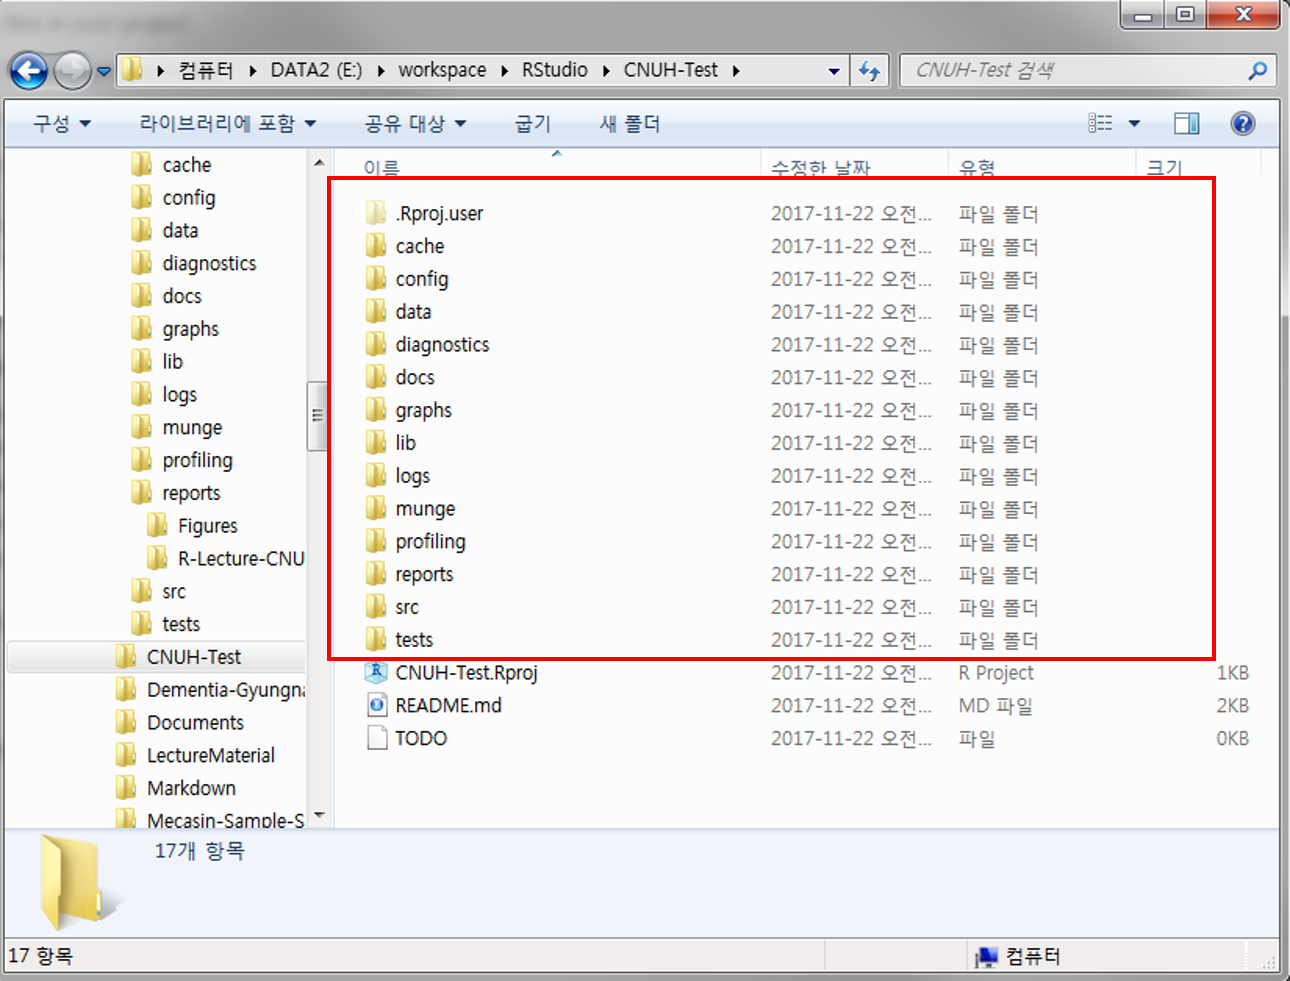
\includegraphics[width = 10cm, height = 8cm]{Figures/R-projecttemplate-01.png}
    \caption[\texttt{create.project()} 후 프로젝트 폴더 내 생성 디렉토리]{\texttt{create.project()} 후 프로젝트 폴더 내 생성 디렉토리}\label{fig:RStudio-projtemp-01}
  } \end{figure}

  \begin{itemize}
  \tightlist
  \item
    \texttt{cache/}: 자료 전처리 과정 중 생성한 cache 처리 데이터 저장
  \item
    \texttt{confing/}: 프로젝트 설정(\texttt{global.gcf}에 저장) 관리
  \item
    \texttt{data/}: 원자료 또는 읽기 전용 분석 자료 저장
  \item
    \texttt{diagnostics/}: 자료의 오류 및 이상치 탐지를 위한 스크립트
    저장
  \item
    \texttt{doc/}: 프로젝트 산출물을 위한 모든 종류의 문서 저장
  \item
    \texttt{graphs/}: 스크립트로 출력된 그래프 저장
  \item
    \texttt{libs/}: 재사용 혹은 자체 제작한 R 함수 스크립트 저장
  \item
    \texttt{munge/}: 자료 전처리를 위한 스크립트 저장
  \item
    \texttt{profiling/}: 코드 실행 시간 체크를 위해 작성산 스크립트 저장
  \item
    \texttt{reports/}: 프로젝트 보고 문서(HTML, PDF 등) 저장
  \item
    \texttt{src/}: 자료분석을 위해 사용한 스크립트 저장
  \item
    \texttt{tests/}: 함수 작성을 위해 생성한 test 스크립트 저장
  \end{itemize}
\end{enumerate}

\begin{enumerate}
\def\labelenumi{\arabic{enumi}.}
\setcounter{enumi}{2}
\tightlist
\item
  \texttt{ProjectTemplate} 관리

  \begin{enumerate}
  \def\labelenumii{\arabic{enumii})}
  \tightlist
  \item
    \texttt{ProjectTemplate}는 \texttt{config/global.dcf} 파일로
    프로젝트 불러올 때 옵션 설정 가능
  \end{enumerate}
\end{enumerate}

\footnotesize

\begin{Shaded}
\begin{Highlighting}[]
\NormalTok{version}\OperatorTok{:}\StringTok{ }\FloatTok{0.8} \CommentTok{# 현재 `ProjectTemplate` 버전 정보}
\NormalTok{data_loading}\OperatorTok{:}\StringTok{ }\OtherTok{TRUE} \CommentTok{# 'data/' 폴더 내 자료읽기 여부 }
\NormalTok{data_loading_header}\OperatorTok{:}\StringTok{ }\OtherTok{TRUE} \CommentTok{# 'data/' 폴더 내 자료읽기 여부 }
\NormalTok{data_ignore}\OperatorTok{:}\StringTok{ }\CommentTok{# 'data/' 폴더 내 읽기무시 파일 목록}
\NormalTok{cache_loading}\OperatorTok{:}\StringTok{ }\OtherTok{TRUE} \CommentTok{# 'cache/' 자료읽기 여부}
\NormalTok{recursive_loading}\OperatorTok{:}\StringTok{ }\OtherTok{FALSE}
\NormalTok{munging}\OperatorTok{:}\StringTok{ }\OtherTok{TRUE} \CommentTok{# 'munging/' 자료전처리 스크립트 읽기여부}
\NormalTok{logging}\OperatorTok{:}\StringTok{ }\OtherTok{FALSE} \CommentTok{# Log 정보 기록여부 }
\NormalTok{logging_level}\OperatorTok{:}\StringTok{ }\NormalTok{INFO}
\NormalTok{load_libraries}\OperatorTok{:}\StringTok{ }\OtherTok{FALSE} \CommentTok{# 아래 패키지 리스트 불러오기 여부}
\NormalTok{libraries}\OperatorTok{:}\StringTok{ }\NormalTok{reshape, plyr, dplyr, ggplot2, stringr, lubridate}
\NormalTok{as_factors}\OperatorTok{:}\StringTok{ }\OtherTok{TRUE} \CommentTok{# 문자형 변수 요인화 여부}
\NormalTok{data_tables}\OperatorTok{:}\StringTok{ }\OtherTok{FALSE} \CommentTok{# data.frame에 data.table 속성 추가}
\NormalTok{attach_internal_libraries}\OperatorTok{:}\StringTok{ }\OtherTok{FALSE} \CommentTok{# 'lib\textbackslash{}'에 저장된 자체 생성 함수 읽기 여부}
\NormalTok{cache_loaded_data}\OperatorTok{:}\StringTok{  }\OtherTok{TRUE} 
\NormalTok{sticky_variables}\OperatorTok{:}\StringTok{ }\NormalTok{NONE}
\end{Highlighting}
\end{Shaded}

\normalsize

\chapter{R의 기본 사용}\label{r--}

\begin{quote}
\colorbox{gray!10}{\begin{minipage}{15cm}
\textbf{목적: R 활용을 위해 기초적으로 알아야 할 객체 속성 및 기본 연산 논리 학습}
\end{minipage}}
\end{quote}

\vspace{0.5cm}

\begin{itemize}
\tightlist
\item
  R은 객체지향언어(object-oriented language)
\item
  객체: 숫자, 데이터셋, 단어, 테이블, 분석결과 등 모든 것을 칭함

  \begin{itemize}
  \tightlist
  \item
    ``객체지향''의 의미는 R의 모든 명령어는 객체를 대상으로 이루어진다는
    것을 의미
  \end{itemize}
\item
  R에서 사용자가 데이터 입력을 위해 생성 또는 읽어온 객체(object)는 종종
  변수(variable)라는 말과 혼용됨.
\item
  본 문서에서는 최상위 데이터 저장장소를 객체라고 명명하며
  데이터프레임과 같이 여러 종류의 데이터타입으로 이루어진 객체의 1차원
  속성을 변수라고 칭함.
\item
  R을 다룰 수 있으려면 기본적인 R의 데이터 할당 방식과 데이터 타입,
  그리고 연산 방법에 대한 이해가 있어야 함.
\item
  특히 데이터 타입에 따라 사용하는 함수 또는 분석 방법이 조금씩 다른
  것이 R의 특징임
\item
  따라서 R의 데이터 타입에 좀 더 익숙해져야 R을 보다 쉽게 다룰 수 있음
\end{itemize}

\section{R의 기초}\label{r-}

\subsection{R 객체 입력 방법 및 변수 설정 규칙}\label{r-------}

R의 가장 기본적인 데이터 입력 및 할당 방법과 객체 또는 변수의 명명 규칙
설명

\begin{enumerate}
\def\labelenumi{\arabic{enumi}.}
\tightlist
\item
  객체를 할당하는 두 가지 방법:\texttt{=}, \texttt{\textless{}-}

  \begin{enumerate}
  \def\labelenumii{\arabic{enumii})}
  \tightlist
  \item
    두 할당 지시자의 차이점

    \begin{itemize}
    \tightlist
    \item
      \texttt{=}: 명령의 최상 수준에사만 사용 가능
    \item
      \texttt{\textless{}-}: 어디서든 사용 가능
    \item
      함수 호출과 동시에 변수에 값을 할당할 목적으로는
      \texttt{\textless{}-}만 사용 가능
    \end{itemize}
  \end{enumerate}
\end{enumerate}

\footnotesize

\begin{Shaded}
\begin{Highlighting}[]
\CommentTok{# 이전 히스토그램 생성 위해 생성한 x 삭제}
\KeywordTok{rm}\NormalTok{(x)}
\CommentTok{# `mean()` 입력 벡터의 평균 계산}
\KeywordTok{mean}\NormalTok{(y <-}\StringTok{ }\KeywordTok{c}\NormalTok{(}\DecValTok{1}\NormalTok{, }\DecValTok{2}\NormalTok{, }\DecValTok{3}\NormalTok{, }\DecValTok{4}\NormalTok{, }\DecValTok{5}\NormalTok{))}
\end{Highlighting}
\end{Shaded}

\begin{verbatim}
[1] 3
\end{verbatim}

\begin{Shaded}
\begin{Highlighting}[]
\NormalTok{y}
\end{Highlighting}
\end{Shaded}

\begin{verbatim}
[1] 1 2 3 4 5
\end{verbatim}

\begin{Shaded}
\begin{Highlighting}[]
\KeywordTok{mean}\NormalTok{(}\DataTypeTok{x =} \KeywordTok{c}\NormalTok{(}\DecValTok{1}\NormalTok{, }\DecValTok{2}\NormalTok{, }\DecValTok{3}\NormalTok{, }\DecValTok{4}\NormalTok{, }\DecValTok{5}\NormalTok{))}
\end{Highlighting}
\end{Shaded}

\begin{verbatim}
[1] 3
\end{verbatim}

\begin{Shaded}
\begin{Highlighting}[]
\NormalTok{x}
\end{Highlighting}
\end{Shaded}

\begin{verbatim}
Error in eval(expr, envir, enclos): 객체 'x'를 찾을 수 없습니다
\end{verbatim}

\normalsize

\begin{enumerate}
\def\labelenumi{\arabic{enumi}.}
\setcounter{enumi}{1}
\tightlist
\item
  객체 또는 변수의 명명 규칙

  \begin{enumerate}
  \def\labelenumii{\arabic{enumii})}
  \tightlist
  \item
    알파벳, 한글, 숫자, \texttt{\_}, \texttt{.}의 조합으로 구성
    가능(\texttt{-}은 사용 불가)
  \item
    변수명의 알파벳, 한글, \texttt{.}로 시작 가능

    \begin{itemize}
    \tightlist
    \item
      \texttt{.}로 시작한 경우 뒤에 숫자 올 수 없음(숫자로 인지)
    \end{itemize}
  \item
    대소문자 구분 \footnotesize
  \end{enumerate}
\end{enumerate}

\begin{Shaded}
\begin{Highlighting}[]
\CommentTok{# 1:10은 1부터 10까지 정수 생성 'c()'는 벡터 생성 함수}
\NormalTok{x <-}\StringTok{ }\KeywordTok{c}\NormalTok{(}\DecValTok{1}\OperatorTok{:}\DecValTok{10}\NormalTok{)}
\CommentTok{# 1:10으로 구성된 행렬 생성}
\NormalTok{X <-}\StringTok{ }\KeywordTok{matrix}\NormalTok{(}\KeywordTok{c}\NormalTok{(}\DecValTok{1}\OperatorTok{:}\DecValTok{10}\NormalTok{), }\DataTypeTok{nrow =} \DecValTok{2}\NormalTok{, }\DataTypeTok{ncol =} \DecValTok{5}\NormalTok{, }\DataTypeTok{byrow =}\NormalTok{ T)}
\NormalTok{x}
\end{Highlighting}
\end{Shaded}

\begin{verbatim}
 [1]  1  2  3  4  5  6  7  8  9 10
\end{verbatim}

\begin{Shaded}
\begin{Highlighting}[]
\NormalTok{X}
\end{Highlighting}
\end{Shaded}

\begin{verbatim}
     [,1] [,2] [,3] [,4] [,5]
[1,]    1    2    3    4    5
[2,]    6    7    8    9   10
\end{verbatim}

\begin{Shaded}
\begin{Highlighting}[]
\CommentTok{# 논리형 객체}
\NormalTok{.x <-}\StringTok{ }\OtherTok{TRUE}
\NormalTok{.x}
\end{Highlighting}
\end{Shaded}

\begin{verbatim}
[1] TRUE
\end{verbatim}

\begin{Shaded}
\begin{Highlighting}[]
\CommentTok{# 알파벳 + 숫자}
\NormalTok{a1 <-}\StringTok{ }\KeywordTok{seq}\NormalTok{(}\DataTypeTok{from =} \DecValTok{1}\NormalTok{, }\DataTypeTok{to =} \DecValTok{10}\NormalTok{, }\DataTypeTok{by =} \DecValTok{2}\NormalTok{)}
\CommentTok{# 한글 변수명}
\NormalTok{가수 <-}\StringTok{ }\KeywordTok{c}\NormalTok{(}\StringTok{"Damian Rice"}\NormalTok{, }\StringTok{"Beatles"}\NormalTok{, }\StringTok{"최백호"}\NormalTok{, }\StringTok{"Queen"}\NormalTok{)}
\NormalTok{가수}
\end{Highlighting}
\end{Shaded}

\begin{verbatim}
[1] "Damian Rice" "Beatles"     "최백호"      "Queen"      
\end{verbatim}

\normalsize

\begin{enumerate}
\def\labelenumi{\arabic{enumi}.}
\setcounter{enumi}{2}
\tightlist
\item
  잘못된 객체 또는 변수 명명 예시 \footnotesize
\end{enumerate}

\begin{Shaded}
\begin{Highlighting}[]
\NormalTok{3x <-}\StringTok{ }\DecValTok{7}
\end{Highlighting}
\end{Shaded}

\begin{verbatim}
Error: <text>:1:2: 예상하지 못한 기호(symbol)입니다.
1: 3x
     ^
\end{verbatim}

\normalsize

\footnotesize

\begin{Shaded}
\begin{Highlighting}[]
\NormalTok{_x <-}\StringTok{ }\KeywordTok{c}\NormalTok{(}\StringTok{"M"}\NormalTok{, }\StringTok{"M"}\NormalTok{, }\StringTok{"F"}\NormalTok{)}
\end{Highlighting}
\end{Shaded}

\begin{verbatim}
Error: <text>:1:1: 예상하지 못한 입력입니다.
1: _
    ^
\end{verbatim}

\normalsize

\footnotesize

\begin{Shaded}
\begin{Highlighting}[]
\FloatTok{0.3}\NormalTok{ <-}\StringTok{ }\DecValTok{10}
\end{Highlighting}
\end{Shaded}

\begin{verbatim}
Error in 0.3 <- 10: 대입에 유효하지 않은 (do_set) 좌변입니다
\end{verbatim}

\normalsize

\section{R 객체 유형}\label{r--}

\begin{enumerate}
\def\labelenumi{\arabic{enumi}.}
\tightlist
\item
  객체의 종류
\end{enumerate}

\begin{itemize}
\tightlist
\item
  스칼라(scalar)
\item
  벡터(vector): \textbf{R의 기본연산 단위}
\item
  행렬(matrix)
\item
  배열(array)
\item
  데이터프레임(data frame)
\item
  리스트(list)
\end{itemize}

\begin{enumerate}
\def\labelenumi{\arabic{enumi}.}
\setcounter{enumi}{1}
\tightlist
\item
  객체에 입력 가능한 값
\end{enumerate}

\begin{itemize}
\item
  \textbf{수치형(numeric)}: 숫자(정수, 소수)
\item
  \textbf{문자열(string)}: \texttt{"충남대학교"}, \texttt{"R강의"}
\item
  \textbf{논리형(logical)}: \texttt{TRUE}/\texttt{FALSE}
\item
  \textbf{결측값(\texttt{NA})}: 자료에서 발생한 결측 표현
\item
  \textbf{공백(\texttt{NULL})}: 지정하지 않은 값
\item
  \textbf{요인(factor)}: 범주형 자료 표현(수치 + 문자 결합 형태로
  이해하면 편함)
\item
  \textbf{기타}: 숫자아님(\texttt{NaN}), 무한대(\texttt{Inf}) 등
\end{itemize}

\subsection{스칼라}

\begin{enumerate}
\def\labelenumi{\arabic{enumi}.}
\tightlist
\item
  단일 차원의 값(하나의 값): \(1 \times 1\) 벡터로 간주 가능

  \begin{itemize}
  \tightlist
  \item
    R 자료형의 기본은 벡터
  \end{itemize}
\item
  자료형은 크게 숫자형, 문자열, 논리형이 있음
\end{enumerate}

\begin{quote}
\textbf{참고: 스칼라를 입력시 R의 벡터 지정 함수인 \texttt{c()}를 꼭
사용해서 입력할 필요가 없다. 단, 두 개 이상 스칼라면 벡터이므로 꼭 c()를
써야 한다.}
\end{quote}

\subsubsection{\texorpdfstring{숫자형:
수치연산(\texttt{+,\ -,\ *,\ \^{},\ **,\ /,\ \%\%,\ \%/\%})
가능}{숫자형: 수치연산(+, -, *, \^{}, **, /, \%\%, \%/\%) 가능}}\label{----}

\begin{table}[H]
  \centering
  \begingroup\footnotesize
  \caption{R의 수치 연산자 및 기본 수학 함수}
  \begin{tabular}{p{5cm}p{7cm}}
  \toprule
  \textbf{연산자 또는 함수} & \textbf{설명} \\
  \midrule
  \texttt{+, -, *, /} & 사칙연산 \\
  \texttt{n \%\% m} & \texttt{n}을 \texttt{m} 으로 나눈 나머지 \\
  \texttt{n \%/\% m} & \texttt{n}을 \texttt{m} 으로 나눈 몫 \\
  \texttt{n : m} & 정수 \texttt{n} 부터 정수 \texttt{m} 까지 1단위 수열 생성 \\
  \texttt{n\textasciicircum m} & \texttt{n}의 \texttt{m} 승 \\
  \texttt{exp(n)} & 상수 $e$의 \texttt{n} 승 \\
  \texttt{log(x, base = m)} & 밑이 \texttt{m}인 x의 로그값 계산. \texttt{base} 값의 default는 $e$ \\
  \texttt{log2(x), log10(x)} & 각각 밑이 2, 10인 x의 로그값 계산 \\
  \texttt{sin(x), cos(x), tan(x)} & 삼각함수 계산 \\
  \bottomrule
  \end{tabular}
  \endgroup
\end{table}

\footnotesize

\begin{Shaded}
\begin{Highlighting}[]
\OperatorTok{>}\StringTok{ }\CommentTok{# 숫자형 스칼라}
\ErrorTok{>}\StringTok{ }\NormalTok{a <-}\StringTok{ }\DecValTok{3}
\OperatorTok{>}\StringTok{ }\NormalTok{b <-}\StringTok{ }\DecValTok{10}
\OperatorTok{>}\StringTok{ }\NormalTok{a}
\end{Highlighting}
\end{Shaded}

\begin{verbatim}
[1] 3
\end{verbatim}

\begin{Shaded}
\begin{Highlighting}[]
\OperatorTok{>}\StringTok{ }\NormalTok{b}
\end{Highlighting}
\end{Shaded}

\begin{verbatim}
[1] 10
\end{verbatim}

\begin{Shaded}
\begin{Highlighting}[]
\OperatorTok{>}\StringTok{ }\CommentTok{# 덧셈}
\ErrorTok{>}\StringTok{ }\NormalTok{c <-}\StringTok{ }\NormalTok{a }\OperatorTok{+}\StringTok{ }\NormalTok{b}
\OperatorTok{>}\StringTok{ }\NormalTok{c}
\end{Highlighting}
\end{Shaded}

\begin{verbatim}
[1] 13
\end{verbatim}

\begin{Shaded}
\begin{Highlighting}[]
\OperatorTok{>}\StringTok{ }\CommentTok{# 뺄셈}
\ErrorTok{>}\StringTok{ }\NormalTok{d <-}\StringTok{ }\NormalTok{b }\OperatorTok{-}\StringTok{ }\NormalTok{a}
\OperatorTok{>}\StringTok{ }\NormalTok{d}
\end{Highlighting}
\end{Shaded}

\begin{verbatim}
[1] 7
\end{verbatim}

\begin{Shaded}
\begin{Highlighting}[]
\OperatorTok{>}\StringTok{ }\CommentTok{# 곱셈}
\ErrorTok{>}\StringTok{ }\NormalTok{a }\OperatorTok{*}\StringTok{ }\NormalTok{b}
\end{Highlighting}
\end{Shaded}

\begin{verbatim}
[1] 30
\end{verbatim}

\begin{Shaded}
\begin{Highlighting}[]
\OperatorTok{>}\StringTok{ }\CommentTok{# 멱승}
\ErrorTok{>}\StringTok{ }\NormalTok{b}\OperatorTok{^}\NormalTok{a}
\end{Highlighting}
\end{Shaded}

\begin{verbatim}
[1] 1000
\end{verbatim}

\begin{Shaded}
\begin{Highlighting}[]
\OperatorTok{>}\StringTok{ }\NormalTok{b}\OperatorTok{^}\NormalTok{a}
\end{Highlighting}
\end{Shaded}

\begin{verbatim}
[1] 1000
\end{verbatim}

\begin{Shaded}
\begin{Highlighting}[]
\OperatorTok{>}\StringTok{ }\CommentTok{# 나누기}
\ErrorTok{>}\StringTok{ }\NormalTok{b}\OperatorTok{/}\NormalTok{a}
\end{Highlighting}
\end{Shaded}

\begin{verbatim}
[1] 3.33
\end{verbatim}

\begin{Shaded}
\begin{Highlighting}[]
\OperatorTok{>}\StringTok{ }\CommentTok{# 나누기 나머지 반환}
\ErrorTok{>}\StringTok{ }\NormalTok{b}\OperatorTok\NormalTok{a}
\end{Highlighting}
\end{Shaded}

\begin{verbatim}
[1] 1
\end{verbatim}

\begin{Shaded}
\begin{Highlighting}[]
\OperatorTok{>}\StringTok{ }\CommentTok{# 나누기 몫 반환}
\ErrorTok{>}\StringTok{ }\NormalTok{b}\OperatorTok\NormalTok{a}
\end{Highlighting}
\end{Shaded}

\begin{verbatim}
[1] 3
\end{verbatim}

\begin{Shaded}
\begin{Highlighting}[]
\OperatorTok{>}\StringTok{ }\CommentTok{# 연산 우선순위}
\ErrorTok{>}\StringTok{ }\NormalTok{n <-}\StringTok{ }\NormalTok{(}\DecValTok{3} \OperatorTok{+}\StringTok{ }\DecValTok{5}\NormalTok{) }\OperatorTok{*}\StringTok{ }\DecValTok{3} \OperatorTok{-}\StringTok{ }\DecValTok{4}\OperatorTok{^}\DecValTok{2}\OperatorTok{/}\DecValTok{2}
\OperatorTok{>}\StringTok{ }\NormalTok{n}
\end{Highlighting}
\end{Shaded}

\begin{verbatim}
[1] 16
\end{verbatim}

\begin{Shaded}
\begin{Highlighting}[]
\OperatorTok{>}\StringTok{ }\CommentTok{# 수열 생성}
\ErrorTok{>}\StringTok{ }\DecValTok{1}\OperatorTok{:}\DecValTok{10}
\end{Highlighting}
\end{Shaded}

\begin{verbatim}
 [1]  1  2  3  4  5  6  7  8  9 10
\end{verbatim}

\begin{Shaded}
\begin{Highlighting}[]
\OperatorTok{>}\StringTok{ }\DecValTok{10}\OperatorTok{:}\DecValTok{1}
\end{Highlighting}
\end{Shaded}

\begin{verbatim}
 [1] 10  9  8  7  6  5  4  3  2  1
\end{verbatim}

\normalsize

\subsubsection{문자형 스칼라: 수치연산 불가능}\label{---}

\footnotesize

\begin{Shaded}
\begin{Highlighting}[]
\OperatorTok{>}\StringTok{ }\NormalTok{h1 <-}\StringTok{ }\KeywordTok{c}\NormalTok{(}\StringTok{"Hello CNU Hospital CTS."}\NormalTok{)}
\OperatorTok{>}\StringTok{ }\NormalTok{g2 <-}\StringTok{ }\KeywordTok{c}\NormalTok{(}\StringTok{"R is not too difficult."}\NormalTok{)}
\OperatorTok{>}\StringTok{ }\NormalTok{h1}
\end{Highlighting}
\end{Shaded}

\begin{verbatim}
[1] "Hello CNU Hospital CTS."
\end{verbatim}

\begin{Shaded}
\begin{Highlighting}[]
\OperatorTok{>}\StringTok{ }\NormalTok{g2}
\end{Highlighting}
\end{Shaded}

\begin{verbatim}
[1] "R is not too difficult."
\end{verbatim}

\begin{Shaded}
\begin{Highlighting}[]
\OperatorTok{>}\StringTok{ }\NormalTok{h1 }\OperatorTok{+}\StringTok{ }\NormalTok{g2}
\end{Highlighting}
\end{Shaded}

\begin{verbatim}
Error in h1 + g2: 이항연산자에 수치가 아닌 인수입니다
\end{verbatim}

\normalsize

\subsubsection{논리형 스칼라}\label{-}

\begin{itemize}
\tightlist
\item
  \texttt{TRUE,\ T}: 참
\item
  \texttt{FALSE,\ F}: 거짓
\item
  \texttt{\&,\ \&\&\ (AND);\ \textbar{},\ \textbar{}\textbar{}\ (OR);\ !\ (NOT)}
  연산자 사용 가능
\item
  비교연산: 숫자값들의 비교를 통해 논리값 반환

  \begin{itemize}
  \tightlist
  \item
    \texttt{\textgreater{},\ \textless{},\ \textgreater{}=,\ \textless{}=,\ ==,\ !=}
  \item
    문자형 비교 연산은 \texttt{==,\ !=}만 가능
  \end{itemize}
\end{itemize}

\begin{quote}
\textbf{참고 1: 논리형 스칼라도 숫자형 연산 가능하다. 왜냐하면 컴퓨터는
TRUE/FALSE를 1과 0의 숫자로 인식하기 때문이다.}
\end{quote}

\begin{quote}
\textbf{참고 2: 수치 연산자는 스칼라 뿐 아니라 아래에서 다룰 벡터, 행렬,
리스트, 데이터프레임 객체의 연산에 사용 가능하다.}
\end{quote}

\begin{quote}
\textbf{참고 2: \texttt{\&}와 \texttt{\&\&}는 동일하게 AND를 의미하지만
연산 결과가 다르다. \texttt{\&}의 연산 대상이 벡터인 경우 백터 구성 값
각각에 대해 \texttt{\&} 연산을 실행 하지만 \texttt{\&\&}는 한
개(스칼라)에만 논리 연산이 적용된다(아래 예시 참고).}
\end{quote}

\footnotesize

\begin{Shaded}
\begin{Highlighting}[]
\OperatorTok{>}\StringTok{ }\OtherTok{TRUE} \OperatorTok{&}\StringTok{ }\OtherTok{TRUE}
\end{Highlighting}
\end{Shaded}

\begin{verbatim}
[1] TRUE
\end{verbatim}

\begin{Shaded}
\begin{Highlighting}[]
\OperatorTok{>}\StringTok{ }\OtherTok{TRUE} \OperatorTok{&}\StringTok{ }\OtherTok{FALSE}
\end{Highlighting}
\end{Shaded}

\begin{verbatim}
[1] FALSE
\end{verbatim}

\begin{Shaded}
\begin{Highlighting}[]
\OperatorTok{>}\StringTok{ }\OtherTok{TRUE} \OperatorTok{|}\StringTok{ }\OtherTok{TRUE}
\end{Highlighting}
\end{Shaded}

\begin{verbatim}
[1] TRUE
\end{verbatim}

\begin{Shaded}
\begin{Highlighting}[]
\OperatorTok{>}\StringTok{ }\OtherTok{TRUE} \OperatorTok{|}\StringTok{ }\OtherTok{FALSE}
\end{Highlighting}
\end{Shaded}

\begin{verbatim}
[1] TRUE
\end{verbatim}

\begin{Shaded}
\begin{Highlighting}[]
\OperatorTok{>}\StringTok{ }\OperatorTok{!}\OtherTok{TRUE}
\end{Highlighting}
\end{Shaded}

\begin{verbatim}
[1] FALSE
\end{verbatim}

\begin{Shaded}
\begin{Highlighting}[]
\OperatorTok{>}\StringTok{ }\OperatorTok{!}\OtherTok{FALSE}
\end{Highlighting}
\end{Shaded}

\begin{verbatim}
[1] TRUE
\end{verbatim}

\begin{Shaded}
\begin{Highlighting}[]
\OperatorTok{>}\StringTok{ }\CommentTok{# T/F는 각각 TRUE/FALSE의 전역변수}
\ErrorTok{>}\StringTok{ }\NormalTok{T <-}\StringTok{ }\OtherTok{FALSE}
\OperatorTok{>}\StringTok{ }\NormalTok{T}
\end{Highlighting}
\end{Shaded}

\begin{verbatim}
[1] FALSE
\end{verbatim}

\begin{Shaded}
\begin{Highlighting}[]
\OperatorTok{>}\StringTok{ }\OtherTok{TRUE}\NormalTok{ <-}\StringTok{ }\OtherTok{FALSE}
\end{Highlighting}
\end{Shaded}

\begin{verbatim}
Error in TRUE <- FALSE: 대입에 유효하지 않은 (do_set) 좌변입니다
\end{verbatim}

\begin{Shaded}
\begin{Highlighting}[]
\OperatorTok{>}\StringTok{ }\NormalTok{T <-}\StringTok{ }\OtherTok{TRUE}
\OperatorTok{>}\StringTok{ }\CommentTok{# &와 &&의 차이}
\ErrorTok{>}\StringTok{ }\NormalTok{l1 <-}\StringTok{ }\KeywordTok{c}\NormalTok{(}\OtherTok{TRUE}\NormalTok{, }\OtherTok{TRUE}\NormalTok{, }\OtherTok{FALSE}\NormalTok{, }\OtherTok{TRUE}\NormalTok{)}
\OperatorTok{>}\StringTok{ }\NormalTok{l2 <-}\StringTok{ }\KeywordTok{c}\NormalTok{(}\OtherTok{FALSE}\NormalTok{, }\OtherTok{TRUE}\NormalTok{, }\OtherTok{TRUE}\NormalTok{, }\OtherTok{TRUE}\NormalTok{)}
\OperatorTok{>}\StringTok{ }\NormalTok{l1 }\OperatorTok{&}\StringTok{ }\NormalTok{l2}
\end{Highlighting}
\end{Shaded}

\begin{verbatim}
[1] FALSE  TRUE FALSE  TRUE
\end{verbatim}

\begin{Shaded}
\begin{Highlighting}[]
\OperatorTok{>}\StringTok{ }\NormalTok{l1 }\OperatorTok{&&}\StringTok{ }\NormalTok{l2}
\end{Highlighting}
\end{Shaded}

\begin{verbatim}
[1] FALSE
\end{verbatim}

\begin{Shaded}
\begin{Highlighting}[]
\OperatorTok{>}\StringTok{ }\NormalTok{x <-}\StringTok{ }\DecValTok{10}
\OperatorTok{>}\StringTok{ }\NormalTok{y <-}\StringTok{ }\DecValTok{13}
\OperatorTok{>}\StringTok{ }\NormalTok{x }\OperatorTok{>}\StringTok{ }\NormalTok{y}
\end{Highlighting}
\end{Shaded}

\begin{verbatim}
[1] FALSE
\end{verbatim}

\begin{Shaded}
\begin{Highlighting}[]
\OperatorTok{>}\StringTok{ }\NormalTok{x }\OperatorTok{<}\StringTok{ }\NormalTok{y}
\end{Highlighting}
\end{Shaded}

\begin{verbatim}
[1] TRUE
\end{verbatim}

\begin{Shaded}
\begin{Highlighting}[]
\OperatorTok{>}\StringTok{ }\NormalTok{x }\OperatorTok{>=}\StringTok{ }\NormalTok{y}
\end{Highlighting}
\end{Shaded}

\begin{verbatim}
[1] FALSE
\end{verbatim}

\begin{Shaded}
\begin{Highlighting}[]
\OperatorTok{>}\StringTok{ }\NormalTok{x }\OperatorTok{<=}\StringTok{ }\NormalTok{y}
\end{Highlighting}
\end{Shaded}

\begin{verbatim}
[1] TRUE
\end{verbatim}

\begin{Shaded}
\begin{Highlighting}[]
\OperatorTok{>}\StringTok{ }\NormalTok{x }\OperatorTok{==}\StringTok{ }\NormalTok{y}
\end{Highlighting}
\end{Shaded}

\begin{verbatim}
[1] FALSE
\end{verbatim}

\begin{Shaded}
\begin{Highlighting}[]
\OperatorTok{>}\StringTok{ }\NormalTok{x }\OperatorTok{!=}\StringTok{ }\NormalTok{y}
\end{Highlighting}
\end{Shaded}

\begin{verbatim}
[1] TRUE
\end{verbatim}

\begin{Shaded}
\begin{Highlighting}[]
\OperatorTok{>}\StringTok{ }\NormalTok{y <-}\StringTok{ }\DecValTok{10}
\OperatorTok{>}\StringTok{ }\NormalTok{x }\OperatorTok{!=}\StringTok{ }\NormalTok{y}
\end{Highlighting}
\end{Shaded}

\begin{verbatim}
[1] FALSE
\end{verbatim}

\normalsize

\subsubsection{\texorpdfstring{결측값(\texttt{NA})}{결측값(NA)}}\label{na}

\begin{itemize}
\tightlist
\item
  데이터 값이 없음을 의미
\item
  예를 들어 4명의 학생 중 3명의 수학 시험 점수가 80, 95, 90 점인데 한
  학생의 점수를 모르는 경우 \texttt{NA}를 이용해 점수 표현
\item
  \texttt{is.na()} 함수를 이용해 해당 값이 결측을 포함하고 있는지 확인
\end{itemize}

\footnotesize

\begin{Shaded}
\begin{Highlighting}[]
\OperatorTok{>}\StringTok{ }\NormalTok{one <-}\StringTok{ }\DecValTok{80}
\OperatorTok{>}\StringTok{ }\NormalTok{two <-}\StringTok{ }\DecValTok{90}
\OperatorTok{>}\StringTok{ }\NormalTok{three <-}\StringTok{ }\DecValTok{75}
\OperatorTok{>}\StringTok{ }\NormalTok{four <-}\StringTok{ }\OtherTok{NA}
\OperatorTok{>}\StringTok{ }\NormalTok{four}
\end{Highlighting}
\end{Shaded}

\begin{verbatim}
[1] NA
\end{verbatim}

\begin{Shaded}
\begin{Highlighting}[]
\OperatorTok{>}\StringTok{ }\CommentTok{# 'is.na()' 결측 NA가 포함되어 있으면 TRUE}
\ErrorTok{>}\StringTok{ }\KeywordTok{is.na}\NormalTok{(}\OtherTok{NA}\NormalTok{)}
\end{Highlighting}
\end{Shaded}

\begin{verbatim}
[1] TRUE
\end{verbatim}

\normalsize

\begin{quote}
참고: 자료에 \texttt{NA}가 포함된 경우 연산 결과는 모두 \texttt{NA}로
변환
\end{quote}

\footnotesize

\begin{Shaded}
\begin{Highlighting}[]
\OtherTok{NA} \OperatorTok{+}\StringTok{ }\DecValTok{1}
\end{Highlighting}
\end{Shaded}

\begin{verbatim}
[1] NA
\end{verbatim}

\begin{Shaded}
\begin{Highlighting}[]
\OtherTok{NA} \OperatorTok{&}\StringTok{ }\OtherTok{TRUE}
\end{Highlighting}
\end{Shaded}

\begin{verbatim}
[1] NA
\end{verbatim}

\normalsize

\begin{itemize}
\tightlist
\item
  위 문제점을 해결하기 위해 R에서 사용하는 대부분의 함수는
  \texttt{na.rm}을 인자로 받음

  \begin{itemize}
  \tightlist
  \item
    \texttt{na.rm}은 \texttt{TRUE} 또는 \texttt{FALSE} 값을 가지며
    결측값을 연산에서 제외할지를 지정함
  \end{itemize}
\end{itemize}

\footnotesize

\begin{Shaded}
\begin{Highlighting}[]
\NormalTok{x <-}\StringTok{ }\KeywordTok{c}\NormalTok{(}\DecValTok{1}\OperatorTok{:}\DecValTok{10}\NormalTok{, }\OtherTok{NA}\NormalTok{)}
\KeywordTok{mean}\NormalTok{(x)  }\CommentTok{# 결측 포함한 연산}
\end{Highlighting}
\end{Shaded}

\begin{verbatim}
[1] NA
\end{verbatim}

\begin{Shaded}
\begin{Highlighting}[]
\CommentTok{# 연산에서 결측 제외(na.rm = TRUE)}
\KeywordTok{mean}\NormalTok{(x, }\DataTypeTok{na.rm =} \OtherTok{TRUE}\NormalTok{)}
\end{Highlighting}
\end{Shaded}

\begin{verbatim}
[1] 5.5
\end{verbatim}

\normalsize

\begin{itemize}
\tightlist
\item
  결측(\texttt{NA}) 처리 함수: \texttt{NA} 값에 따라 처리를 다르게 하기
  위한 함수

  \begin{itemize}
  \tightlist
  \item
    \texttt{na.fail}, \texttt{na.omit}, \texttt{na.exclude},
    \texttt{na.pass}
  \item
    보통 R의 선형모형과 관련된 함수에서 사용되며, 이들 함수의
    \texttt{na.action}에 대한 인자값으로 사용됨
  \end{itemize}
\end{itemize}

\begin{table}[H]
  \centering
  \begingroup\footnotesize
  \caption{\texttt{NA} 처리 함수}
  \begin{tabular}{p{5cm}p{9cm}}
  \toprule
  \textbf{함수} & \textbf{설명} \\
  \midrule
  \texttt{na.fail(<object>, ...)} & \texttt{<object>}에 \texttt{NA}가 포함되어 있으면 에러 반환 \\
  \texttt{na.omit(<object>, ...)} & \texttt{<object>}에 \texttt{NA}가 포함되어 있으면 생략 \\
  \texttt{na.exclude(<object>, ...)} & \texttt{na.omit()}과 동일하게 작동하지만, 선형모형 관련 함수 중 잔차나 예측값을 반환하는  `resid`, `predict` 함수에서 `NA`로 제외한 행을 출력결과에 다시 추가 \\
  \texttt{na.pass(<object>, ...)} & \texttt{<object>}에 NA가 포함되더라도 통과 \\
  \bottomrule
  \end{tabular}
  \endgroup
\end{table}

\subsubsection{\texorpdfstring{NULL
값(\texttt{NULL})}{NULL 값(NULL)}}\label{null-null}

\begin{itemize}
\tightlist
\item
  초기화 되지 않은 값 표현
\item
  \texttt{is.null()} 함수를 통해 NULL 지정 여부 확인
\end{itemize}

\begin{quote}
\colorbox{gray!10}{\begin{minipage}{15cm}
\textbf{참고: \texttt{NA}와 \texttt{NULL}은 자료의 공백을 의미한다는 점에서 유사한 측면이 있으나 아래 측면에서 큰 차이가 있음!!}
\begin{itemize}
  \item \texttt{NULL}: 값을 지정하지 않은 객체(object) 표현
  \item \texttt{NA}: 자료값이 결측임을 지정해주는 논리형 상수
\end{itemize}
\end{minipage}}
\end{quote}

\vspace{0.5cm}

\footnotesize

\begin{Shaded}
\begin{Highlighting}[]
\OperatorTok{>}\StringTok{ }\CommentTok{# NA와 NULL의 차이점 'is.null()' 객체 또는 변수에 NULL이 저장되어 있는지 판단}
\ErrorTok{>}\StringTok{ }\CommentTok{# 'class()' 객체의 유형을 반환}
\ErrorTok{>}\StringTok{ }\NormalTok{x <-}\StringTok{ }\OtherTok{NULL}
\OperatorTok{>}\StringTok{ }\KeywordTok{is.null}\NormalTok{(x)}
\end{Highlighting}
\end{Shaded}

\begin{verbatim}
[1] TRUE
\end{verbatim}

\begin{Shaded}
\begin{Highlighting}[]
\OperatorTok{>}\StringTok{ }\KeywordTok{is.null}\NormalTok{(}\DecValTok{1}\NormalTok{)}
\end{Highlighting}
\end{Shaded}

\begin{verbatim}
[1] FALSE
\end{verbatim}

\begin{Shaded}
\begin{Highlighting}[]
\OperatorTok{>}\StringTok{ }\KeywordTok{is.null}\NormalTok{(}\OtherTok{NA}\NormalTok{)}
\end{Highlighting}
\end{Shaded}

\begin{verbatim}
[1] FALSE
\end{verbatim}

\begin{Shaded}
\begin{Highlighting}[]
\OperatorTok{>}\StringTok{ }\KeywordTok{is.na}\NormalTok{(}\OtherTok{NULL}\NormalTok{)}
\end{Highlighting}
\end{Shaded}

\begin{verbatim}
logical(0)
\end{verbatim}

\begin{Shaded}
\begin{Highlighting}[]
\OperatorTok{>}\StringTok{ }\KeywordTok{class}\NormalTok{(}\OtherTok{NA}\NormalTok{)}
\end{Highlighting}
\end{Shaded}

\begin{verbatim}
[1] "logical"
\end{verbatim}

\begin{Shaded}
\begin{Highlighting}[]
\OperatorTok{>}\StringTok{ }\KeywordTok{class}\NormalTok{(}\OtherTok{NULL}\NormalTok{)}
\end{Highlighting}
\end{Shaded}

\begin{verbatim}
[1] "NULL"
\end{verbatim}

\normalsize

\subsubsection{요인형}

\begin{itemize}
\tightlist
\item
  범주형 자료를 표현하기 위한 값
\item
  범주형 자료
\item
  데이터가 사전에 정해진 특정 유형으로만 분류되는 경우 - 성별, 인종,
  혈액형 등

  \begin{itemize}
  \tightlist
  \item
    범주형 자료는 명목형과 순서형으로 구분 가능

    \begin{itemize}
    \tightlist
    \item
      순서형 자료 예: 성적, 교육수준, 선호도, 중증도 등
    \end{itemize}
  \end{itemize}
\item
  \texttt{factor()} 함수를 통해 표현 가능

  \begin{itemize}
  \tightlist
  \item
    프로토타입: \texttt{factor(x,\ levels,\ labels,\ ordered)}
    (\texttt{help(factor)} 참조)

    \begin{itemize}
    \tightlist
    \item
      \texttt{x} 벡터(스칼라)에 대응하는 요인의 수준(\texttt{levels})과
      수준의 레이블(\texttt{labels})을 지정. 만약 요인 \texttt{x}가
      순서형이면 \texttt{ordered}인지 아닌지를 입력
    \end{itemize}
  \item
    숫자형에 적용되는 연산 불가
  \item
    요인형을 조금 더 부연설명 하면 숫자 또는 문자 값에 수준의 속성을
    부여한 값의 형태임
  \end{itemize}
\end{itemize}

\begin{quote}
\colorbox{gray!10}{\begin{minipage}{15cm}
\textbf{예시 사용 함수}
\begin{itemize}
  \item \texttt{is.factor()}: 벡터(스칼라)가 요인형인지 확인
  \item \texttt{nlevels()}: factor의 level 개수 반환
  \item \texttt{levels()}: level 목록 반환
  \item \texttt{labels()}: level에 대응하는 label 목록 반환
  \item \texttt{ordered()}: 순서형 factor 생성
  \item \texttt{is.ordered()}: 순서형 factor 확인
\end{itemize}
\end{minipage}}
\end{quote}

\vspace{0.5cm}

\footnotesize

\begin{Shaded}
\begin{Highlighting}[]
\OperatorTok{>}\StringTok{ }\CommentTok{# factor() 기본 사용법 factor(x, levels, labels, ordered = F) x: factor 형으로}
\ErrorTok{>}\StringTok{ }\CommentTok{# 지정하고자 하는 스칼라 또는 벡터 levels: factor의 수준 지정 labels: factor의 레이블}
\ErrorTok{>}\StringTok{ }\CommentTok{# 지정}
\ErrorTok{>}\StringTok{ }\NormalTok{sex <-}\StringTok{ }\KeywordTok{factor}\NormalTok{(}\StringTok{"M"}\NormalTok{, }\DataTypeTok{levels =} \KeywordTok{c}\NormalTok{(}\StringTok{"M"}\NormalTok{, }\StringTok{"F"}\NormalTok{))}
\OperatorTok{>}\StringTok{ }\NormalTok{sex}
\end{Highlighting}
\end{Shaded}

\begin{verbatim}
[1] M
Levels: M F
\end{verbatim}

\begin{Shaded}
\begin{Highlighting}[]
\OperatorTok{>}\StringTok{ }\CommentTok{# factor 형 판단 TRUE/FALSE}
\ErrorTok{>}\StringTok{ }\KeywordTok{is.factor}\NormalTok{(sex)}
\end{Highlighting}
\end{Shaded}

\begin{verbatim}
[1] TRUE
\end{verbatim}

\begin{Shaded}
\begin{Highlighting}[]
\OperatorTok{>}\StringTok{ }\CommentTok{# factor의 level 개수 반환}
\ErrorTok{>}\StringTok{ }\KeywordTok{nlevels}\NormalTok{(sex)}
\end{Highlighting}
\end{Shaded}

\begin{verbatim}
[1] 2
\end{verbatim}

\begin{Shaded}
\begin{Highlighting}[]
\OperatorTok{>}\StringTok{ }\CommentTok{# factor의 level 목록 반환}
\ErrorTok{>}\StringTok{ }\KeywordTok{levels}\NormalTok{(sex)}
\end{Highlighting}
\end{Shaded}

\begin{verbatim}
[1] "M" "F"
\end{verbatim}

\begin{Shaded}
\begin{Highlighting}[]
\OperatorTok{>}\StringTok{ }\CommentTok{# factor의 level 목록 수정}
\ErrorTok{>}\StringTok{ }\KeywordTok{levels}\NormalTok{(sex) <-}\StringTok{ }\KeywordTok{c}\NormalTok{(}\StringTok{"Male"}\NormalTok{, }\StringTok{"Female"}\NormalTok{)}
\OperatorTok{>}\StringTok{ }\NormalTok{sex}
\end{Highlighting}
\end{Shaded}

\begin{verbatim}
[1] Male
Levels: Male Female
\end{verbatim}

\begin{Shaded}
\begin{Highlighting}[]
\OperatorTok{>}\StringTok{ }\CommentTok{# 순서형 factor}
\ErrorTok{>}\StringTok{ }\NormalTok{severity <-}\StringTok{ }\KeywordTok{factor}\NormalTok{(}\DecValTok{1}\NormalTok{, }\DataTypeTok{levels =} \KeywordTok{c}\NormalTok{(}\DecValTok{1}\NormalTok{, }\DecValTok{2}\NormalTok{, }\DecValTok{3}\NormalTok{), }\DataTypeTok{labels =} \KeywordTok{c}\NormalTok{(}\StringTok{"Mild"}\NormalTok{, }\StringTok{"Moderate"}\NormalTok{, }\StringTok{"Severe"}\NormalTok{))}
\OperatorTok{>}\StringTok{ }\CommentTok{# severity <- ordered(severity) 또는 factor() 함수 내에서 ordered 옵션을 TRUE로 지정}
\ErrorTok{>}\StringTok{ }\NormalTok{severity <-}\StringTok{ }\KeywordTok{factor}\NormalTok{(}\DecValTok{1}\NormalTok{, }\DataTypeTok{levels =} \KeywordTok{c}\NormalTok{(}\DecValTok{1}\NormalTok{, }\DecValTok{2}\NormalTok{, }\DecValTok{3}\NormalTok{), }\DataTypeTok{labels =} \KeywordTok{c}\NormalTok{(}\StringTok{"Mild"}\NormalTok{, }\StringTok{"Moderate"}\NormalTok{, }\StringTok{"Severe"}\NormalTok{), }\DataTypeTok{ordered =} \OtherTok{TRUE}\NormalTok{)}
\OperatorTok{>}\StringTok{ }\NormalTok{severity}
\end{Highlighting}
\end{Shaded}

\begin{verbatim}
[1] Mild
Levels: Mild < Moderate < Severe
\end{verbatim}

\begin{Shaded}
\begin{Highlighting}[]
\OperatorTok{>}\StringTok{ }\KeywordTok{is.ordered}\NormalTok{(severity)}
\end{Highlighting}
\end{Shaded}

\begin{verbatim}
[1] TRUE
\end{verbatim}

\normalsize

\subsection{벡터(vector)}\label{vector}

\begin{itemize}
\tightlist
\item
  동일한 유형의 자료(스칼라)가 2개 이상 1차원 (\(n \times 1\),
  \(n \geq 2\)) 으로 구성되어 있는 자료 형태
\item
  벡터는 앞의 예시에서 본 바와 같이 \texttt{c()} 함수를 사용해 생성
\item
  서로 다른 자료형으로 벡터를 구성한 경우 표현력이 돞은 자료형으로
  변환한 값 반환

  \begin{itemize}
  \tightlist
  \item
    예: 문자열 + 숫자로 구성된 벡터 \(\rightarrow\) 문자형 벡터
  \end{itemize}
\item
  벡터 각 원소에 이름 부여 가능

  \begin{itemize}
  \tightlist
  \item
    \texttt{names()} 함수를 이용해 원소 이름 지정

    \begin{itemize}
    \tightlist
    \item
      사용 프로토타입: \texttt{names(x)\ \textless{}-\ 문자열\ 벡터}, 단
      \texttt{x}와 이름에 입력할 문자열 벡터의 길이는 같아야 함.
    \end{itemize}
  \item
    벡터의 길이(차원) 확인

    \begin{itemize}
    \tightlist
    \item
      \texttt{length()} 또는 \texttt{NROW()} 사용
    \end{itemize}
  \end{itemize}
\item
  색인(indexing)을 통해 벡터의 원소에 접근 가능

  \begin{itemize}
  \tightlist
  \item
    \texttt{x{[}i{]}}: 벡터 \texttt{x}의 \texttt{i}번 째 요소
  \item
    \texttt{x{[}-i{]}}: 벡터 \texttt{x}에서 \texttt{i}번 째 요소를
    제외한 나머지
  \item
    \texttt{x{[}I{]}}: \texttt{I}가 인덱싱 벡터라고 할 때 \texttt{I}에
    지정된 요소를 얻어옴. 일반적으로 \texttt{I}는 백터의 행 순서 번호
    또는 각 벡터 원소의 이름에 대응하는 문자열 벡터를 인덱싱 벡터로
    사용할 수 있음.
  \item
    \texttt{x{[}start:end{]}}: \texttt{x}의 \texttt{start}부터
    \texttt{end}까지 값 반환
  \end{itemize}
\item
  벡터의 원소가 \texttt{NULL}을 포함한 경우 해당 원소가 완전히 삭제(예시
  참조)
\end{itemize}

\footnotesize

\begin{Shaded}
\begin{Highlighting}[]
\CommentTok{# 숫자형 벡터}
\NormalTok{x <-}\StringTok{ }\KeywordTok{c}\NormalTok{(}\DecValTok{1}\OperatorTok{:}\DecValTok{25}\NormalTok{)}
\NormalTok{y <-}\StringTok{ }\KeywordTok{c}\NormalTok{(}\DecValTok{26}\OperatorTok{:}\DecValTok{50}\NormalTok{)}
\KeywordTok{is.numeric}\NormalTok{(x)}
\end{Highlighting}
\end{Shaded}

\begin{verbatim}
[1] TRUE
\end{verbatim}

\begin{Shaded}
\begin{Highlighting}[]
\CommentTok{# 벡터의 연산 사칙연산}
\NormalTok{x }\OperatorTok{+}\StringTok{ }\NormalTok{y}
\end{Highlighting}
\end{Shaded}

\begin{verbatim}
 [1] 27 29 31 33 35 37 39 41 43 45 47 49 51 53 55 57 59 61 63 65 67 69 71 73 75
\end{verbatim}

\begin{Shaded}
\begin{Highlighting}[]
\NormalTok{x }\OperatorTok{-}\StringTok{ }\NormalTok{y}
\end{Highlighting}
\end{Shaded}

\begin{verbatim}
 [1] -25 -25 -25 -25 -25 -25 -25 -25 -25 -25 -25 -25 -25 -25 -25 -25 -25 -25 -25 -25
[21] -25 -25 -25 -25 -25
\end{verbatim}

\begin{Shaded}
\begin{Highlighting}[]
\NormalTok{x}\OperatorTok{/}\NormalTok{y}
\end{Highlighting}
\end{Shaded}

\begin{verbatim}
 [1] 0.0385 0.0741 0.1071 0.1379 0.1667 0.1935 0.2188 0.2424 0.2647 0.2857 0.3056
[12] 0.3243 0.3421 0.3590 0.3750 0.3902 0.4048 0.4186 0.4318 0.4444 0.4565 0.4681
[23] 0.4792 0.4898 0.5000
\end{verbatim}

\begin{Shaded}
\begin{Highlighting}[]
\NormalTok{x }\OperatorTok{*}\StringTok{ }\NormalTok{y}
\end{Highlighting}
\end{Shaded}

\begin{verbatim}
 [1]   26   54   84  116  150  186  224  264  306  350  396  444  494  546  600  656
[17]  714  774  836  900  966 1034 1104 1176 1250
\end{verbatim}

\begin{Shaded}
\begin{Highlighting}[]
\NormalTok{## 비교 연산}
\NormalTok{a <-}\StringTok{ }\KeywordTok{c}\NormalTok{(}\DecValTok{1}\NormalTok{, }\DecValTok{2}\NormalTok{, }\DecValTok{3}\NormalTok{, }\DecValTok{3}\NormalTok{, }\DecValTok{4}\NormalTok{, }\DecValTok{2}\NormalTok{, }\DecValTok{5}\NormalTok{, }\DecValTok{1}\NormalTok{, }\DecValTok{2}\NormalTok{, }\DecValTok{3}\NormalTok{, }\DecValTok{4}\NormalTok{, }\DecValTok{4}\NormalTok{, }\DecValTok{4}\NormalTok{)}
\NormalTok{b <-}\StringTok{ }\KeywordTok{c}\NormalTok{(}\DecValTok{2}\NormalTok{, }\DecValTok{2}\NormalTok{, }\DecValTok{4}\NormalTok{, }\DecValTok{4}\NormalTok{, }\DecValTok{3}\NormalTok{, }\DecValTok{2}\NormalTok{, }\DecValTok{5}\NormalTok{, }\DecValTok{1}\NormalTok{, }\DecValTok{2}\NormalTok{, }\DecValTok{4}\NormalTok{, }\DecValTok{4}\NormalTok{, }\DecValTok{4}\NormalTok{, }\DecValTok{3}\NormalTok{)}
\NormalTok{a }\OperatorTok{>}\StringTok{ }\NormalTok{b}
\end{Highlighting}
\end{Shaded}

\begin{verbatim}
 [1] FALSE FALSE FALSE FALSE  TRUE FALSE FALSE FALSE FALSE FALSE FALSE FALSE  TRUE
\end{verbatim}

\begin{Shaded}
\begin{Highlighting}[]
\NormalTok{a }\OperatorTok{>=}\StringTok{ }\NormalTok{b}
\end{Highlighting}
\end{Shaded}

\begin{verbatim}
 [1] FALSE  TRUE FALSE FALSE  TRUE  TRUE  TRUE  TRUE  TRUE FALSE  TRUE  TRUE  TRUE
\end{verbatim}

\begin{Shaded}
\begin{Highlighting}[]
\NormalTok{a }\OperatorTok{<}\StringTok{ }\NormalTok{b}
\end{Highlighting}
\end{Shaded}

\begin{verbatim}
 [1]  TRUE FALSE  TRUE  TRUE FALSE FALSE FALSE FALSE FALSE  TRUE FALSE FALSE FALSE
\end{verbatim}

\begin{Shaded}
\begin{Highlighting}[]
\NormalTok{a }\OperatorTok{<=}\StringTok{ }\NormalTok{b}
\end{Highlighting}
\end{Shaded}

\begin{verbatim}
 [1]  TRUE  TRUE  TRUE  TRUE FALSE  TRUE  TRUE  TRUE  TRUE  TRUE  TRUE  TRUE FALSE
\end{verbatim}

\begin{Shaded}
\begin{Highlighting}[]
\NormalTok{a }\OperatorTok{==}\StringTok{ }\NormalTok{b}
\end{Highlighting}
\end{Shaded}

\begin{verbatim}
 [1] FALSE  TRUE FALSE FALSE FALSE  TRUE  TRUE  TRUE  TRUE FALSE  TRUE  TRUE FALSE
\end{verbatim}

\begin{Shaded}
\begin{Highlighting}[]
\NormalTok{a }\OperatorTok{!=}\StringTok{ }\NormalTok{b}
\end{Highlighting}
\end{Shaded}

\begin{verbatim}
 [1]  TRUE FALSE  TRUE  TRUE  TRUE FALSE FALSE FALSE FALSE  TRUE FALSE FALSE  TRUE
\end{verbatim}

\begin{Shaded}
\begin{Highlighting}[]
\CommentTok{# 벡터의 길이: `length()` 또는 `NROW` 함수 이용}
\NormalTok{z <-}\StringTok{ }\DecValTok{1}
\KeywordTok{length}\NormalTok{(z)}
\end{Highlighting}
\end{Shaded}

\begin{verbatim}
[1] 1
\end{verbatim}

\begin{Shaded}
\begin{Highlighting}[]
\KeywordTok{NROW}\NormalTok{(x)}
\end{Highlighting}
\end{Shaded}

\begin{verbatim}
[1] 25
\end{verbatim}

\begin{Shaded}
\begin{Highlighting}[]
\CommentTok{# 문자형 벡터}
\NormalTok{str1 <-}\StringTok{ }\KeywordTok{c}\NormalTok{(}\StringTok{"Boncho Ku"}\NormalTok{, }\StringTok{"Linear Regression"}\NormalTok{, }\StringTok{"307"}\NormalTok{, }\StringTok{"Male"}\NormalTok{)}
\NormalTok{str1}
\end{Highlighting}
\end{Shaded}

\begin{verbatim}
[1] "Boncho Ku"         "Linear Regression" "307"               "Male"             
\end{verbatim}

\begin{Shaded}
\begin{Highlighting}[]
\CommentTok{# 벡터 원소의 이름 지정}
\KeywordTok{names}\NormalTok{(str1) <-}\StringTok{ }\KeywordTok{c}\NormalTok{(}\StringTok{"Name"}\NormalTok{, }\StringTok{"Subject"}\NormalTok{, }\StringTok{"Room"}\NormalTok{, }\StringTok{"Sex"}\NormalTok{)}
\NormalTok{str1}
\end{Highlighting}
\end{Shaded}

\begin{verbatim}
               Name             Subject                Room                 Sex 
        "Boncho Ku" "Linear Regression"               "307"              "Male" 
\end{verbatim}

\begin{Shaded}
\begin{Highlighting}[]
\KeywordTok{is.numeric}\NormalTok{(str1)}
\end{Highlighting}
\end{Shaded}

\begin{verbatim}
[1] FALSE
\end{verbatim}

\begin{Shaded}
\begin{Highlighting}[]
\KeywordTok{is.character}\NormalTok{(str1)}
\end{Highlighting}
\end{Shaded}

\begin{verbatim}
[1] TRUE
\end{verbatim}

\begin{Shaded}
\begin{Highlighting}[]
\CommentTok{# 숫자와 문자를 동시에 포함한 벡터라면?}
\NormalTok{vec1 <-}\StringTok{ }\KeywordTok{c}\NormalTok{(}\DecValTok{1}\NormalTok{, }\DecValTok{2}\NormalTok{, }\DecValTok{5}\NormalTok{, }\StringTok{"1"}\NormalTok{, }\StringTok{"Clinical Trial"}\NormalTok{)}
\NormalTok{## check: 모든 원소가 문자열로 변환된 것 확인}
\NormalTok{vec1}
\end{Highlighting}
\end{Shaded}

\begin{verbatim}
[1] "1"              "2"              "5"              "1"             
[5] "Clinical Trial"
\end{verbatim}

\begin{Shaded}
\begin{Highlighting}[]
\CommentTok{# 논리형 벡터}
\NormalTok{boolen <-}\StringTok{ }\KeywordTok{c}\NormalTok{(}\OtherTok{TRUE}\NormalTok{, }\OtherTok{TRUE}\NormalTok{, }\OtherTok{FALSE}\NormalTok{, }\OtherTok{TRUE}\NormalTok{, }\OtherTok{TRUE}\NormalTok{, }\OtherTok{TRUE}\NormalTok{, }\OtherTok{FALSE}\NormalTok{, }\OtherTok{FALSE}\NormalTok{)}
\KeywordTok{is.numeric}\NormalTok{(boolen)}
\end{Highlighting}
\end{Shaded}

\begin{verbatim}
[1] FALSE
\end{verbatim}

\begin{Shaded}
\begin{Highlighting}[]
\KeywordTok{is.logical}\NormalTok{(boolen)}
\end{Highlighting}
\end{Shaded}

\begin{verbatim}
[1] TRUE
\end{verbatim}

\begin{Shaded}
\begin{Highlighting}[]
\CommentTok{# 결측을 포함한 벡터}
\NormalTok{vecNA <-}\StringTok{ }\KeywordTok{c}\NormalTok{(}\DecValTok{1}\OperatorTok{:}\DecValTok{10}\NormalTok{, }\OtherTok{NA}\NormalTok{, }\OtherTok{NA}\NormalTok{)}
\KeywordTok{is.na}\NormalTok{(vecNA)}
\end{Highlighting}
\end{Shaded}

\begin{verbatim}
 [1] FALSE FALSE FALSE FALSE FALSE FALSE FALSE FALSE FALSE FALSE  TRUE  TRUE
\end{verbatim}

\begin{Shaded}
\begin{Highlighting}[]
\KeywordTok{is.numeric}\NormalTok{(vecNA)}
\end{Highlighting}
\end{Shaded}

\begin{verbatim}
[1] TRUE
\end{verbatim}

\begin{Shaded}
\begin{Highlighting}[]
\CommentTok{# NULL 포함 벡터}
\NormalTok{vecNULL <-}\StringTok{ }\KeywordTok{c}\NormalTok{(}\OtherTok{NULL}\NormalTok{, }\DecValTok{1}\NormalTok{, }\DecValTok{2}\NormalTok{, }\OtherTok{NULL}\NormalTok{, }\DecValTok{3}\NormalTok{)}
\NormalTok{vecNULL}
\end{Highlighting}
\end{Shaded}

\begin{verbatim}
[1] 1 2 3
\end{verbatim}

\begin{Shaded}
\begin{Highlighting}[]
\CommentTok{# seq_along(), rep() 함수 사용}
\KeywordTok{seq_along}\NormalTok{(x)}
\end{Highlighting}
\end{Shaded}

\begin{verbatim}
 [1]  1  2  3  4  5  6  7  8  9 10 11 12 13 14 15 16 17 18 19 20 21 22 23 24 25
\end{verbatim}

\begin{Shaded}
\begin{Highlighting}[]
\NormalTok{z <-}\StringTok{ }\KeywordTok{c}\NormalTok{(}\DecValTok{3}\NormalTok{, }\DecValTok{8}\NormalTok{)}
\CommentTok{# `rep(x, each)` 사용 예}
\KeywordTok{rep}\NormalTok{(z, }\DataTypeTok{each =} \DecValTok{3}\NormalTok{)}
\end{Highlighting}
\end{Shaded}

\begin{verbatim}
[1] 3 3 3 8 8 8
\end{verbatim}

\begin{Shaded}
\begin{Highlighting}[]
\CommentTok{# `rep(x, times)` 사용 예}
\KeywordTok{rep}\NormalTok{(z, }\DataTypeTok{times =} \DecValTok{3}\NormalTok{)}
\end{Highlighting}
\end{Shaded}

\begin{verbatim}
[1] 3 8 3 8 3 8
\end{verbatim}

\begin{Shaded}
\begin{Highlighting}[]
\CommentTok{# `rep(x, each, times)` 사용 예}
\KeywordTok{rep}\NormalTok{(z, }\DataTypeTok{each =} \DecValTok{2}\NormalTok{, }\DataTypeTok{times =} \DecValTok{3}\NormalTok{)}
\end{Highlighting}
\end{Shaded}

\begin{verbatim}
 [1] 3 3 8 8 3 3 8 8 3 3 8 8
\end{verbatim}

\begin{Shaded}
\begin{Highlighting}[]
\CommentTok{# 요인 벡터 rep() 함수를 이용한 0,1 벡터 생성}
\NormalTok{sex <-}\StringTok{ }\KeywordTok{rep}\NormalTok{(}\KeywordTok{c}\NormalTok{(}\DecValTok{0}\NormalTok{, }\DecValTok{1}\NormalTok{), }\DataTypeTok{each =} \DecValTok{10}\NormalTok{)}
\NormalTok{sex}
\end{Highlighting}
\end{Shaded}

\begin{verbatim}
 [1] 0 0 0 0 0 0 0 0 0 0 1 1 1 1 1 1 1 1 1 1
\end{verbatim}

\begin{Shaded}
\begin{Highlighting}[]
\NormalTok{sex <-}\StringTok{ }\KeywordTok{factor}\NormalTok{(sex, }\DataTypeTok{levels =} \KeywordTok{c}\NormalTok{(}\DecValTok{0}\NormalTok{, }\DecValTok{1}\NormalTok{), }\DataTypeTok{labels =} \KeywordTok{c}\NormalTok{(}\StringTok{"Male"}\NormalTok{, }\StringTok{"Female"}\NormalTok{))}
\NormalTok{sex}
\end{Highlighting}
\end{Shaded}

\begin{verbatim}
 [1] Male   Male   Male   Male   Male   Male   Male   Male   Male   Male   Female
[12] Female Female Female Female Female Female Female Female Female
Levels: Male Female
\end{verbatim}

\begin{Shaded}
\begin{Highlighting}[]
\KeywordTok{str}\NormalTok{(sex)}
\end{Highlighting}
\end{Shaded}

\begin{verbatim}
 Factor w/ 2 levels "Male","Female": 1 1 1 1 1 1 1 1 1 1 ...
\end{verbatim}

\begin{Shaded}
\begin{Highlighting}[]
\CommentTok{# 벡터의 색인}
\NormalTok{x[}\DecValTok{10}\NormalTok{]}
\end{Highlighting}
\end{Shaded}

\begin{verbatim}
[1] 10
\end{verbatim}

\begin{Shaded}
\begin{Highlighting}[]
\NormalTok{x[}\OperatorTok{-}\DecValTok{3}\NormalTok{]}
\end{Highlighting}
\end{Shaded}

\begin{verbatim}
 [1]  1  2  4  5  6  7  8  9 10 11 12 13 14 15 16 17 18 19 20 21 22 23 24 25
\end{verbatim}

\begin{Shaded}
\begin{Highlighting}[]
\NormalTok{x[}\DecValTok{1}\OperatorTok{:}\DecValTok{5}\NormalTok{]}
\end{Highlighting}
\end{Shaded}

\begin{verbatim}
[1] 1 2 3 4 5
\end{verbatim}

\begin{Shaded}
\begin{Highlighting}[]
\NormalTok{x[}\KeywordTok{c}\NormalTok{(}\DecValTok{1}\OperatorTok{:}\DecValTok{3}\NormalTok{, }\DecValTok{10}\OperatorTok{:}\DecValTok{12}\NormalTok{)]}
\end{Highlighting}
\end{Shaded}

\begin{verbatim}
[1]  1  2  3 10 11 12
\end{verbatim}

\begin{Shaded}
\begin{Highlighting}[]
\NormalTok{x[}\OperatorTok{-}\KeywordTok{c}\NormalTok{(}\DecValTok{1}\OperatorTok{:}\DecValTok{10}\NormalTok{)]}
\end{Highlighting}
\end{Shaded}

\begin{verbatim}
 [1] 11 12 13 14 15 16 17 18 19 20 21 22 23 24 25
\end{verbatim}

\begin{Shaded}
\begin{Highlighting}[]
\NormalTok{str1[}\StringTok{"Name"}\NormalTok{]}
\end{Highlighting}
\end{Shaded}

\begin{verbatim}
       Name 
"Boncho Ku" 
\end{verbatim}

\normalsize

\begin{quote}
\colorbox{gray!10}{\begin{minipage}{15cm}
\textbf{알아두면 유용한 벡터 연산자: 벡터는 숫자, 문자열의 묶음, 즉 집합의 개념으로 볼 수 있기 때문에 집합연산이 가능함}
\begin{itemize}
  \item \texttt{identical(x, y)}: 객체 \texttt{x}와 객체 \texttt{y}가 동일한지 판단
  \item \texttt{union(x, y)}: 객체 \texttt{x}와 객체 \texttt{y}의 합집합
  \item \texttt{intersection(x, y)}: 객체 \texttt{x}와 객체 \texttt{y}의 교집합
  \item \texttt{setdiff(x, y)}: 객체 \texttt{x}와 객체 \texttt{y}의 차집합
  \item \texttt{x \%in\% y} :\texttt{y}에 \texttt{x}의 원소가 포함되어 있는지 판단
\end{itemize}
\end{minipage}}
\end{quote}

\vspace{0.5cm} \textbf{벡터의 집합연산 예시}

\footnotesize

\begin{Shaded}
\begin{Highlighting}[]
\NormalTok{x <-}\StringTok{ }\KeywordTok{c}\NormalTok{(}\DecValTok{1}\OperatorTok{:}\DecValTok{3}\NormalTok{)}
\NormalTok{y <-}\StringTok{ }\KeywordTok{c}\NormalTok{(}\DecValTok{1}\OperatorTok{:}\DecValTok{3}\NormalTok{)}
\KeywordTok{identical}\NormalTok{(x, y)}
\end{Highlighting}
\end{Shaded}

\begin{verbatim}
[1] TRUE
\end{verbatim}

\begin{Shaded}
\begin{Highlighting}[]
\NormalTok{y <-}\StringTok{ }\KeywordTok{c}\NormalTok{(}\DecValTok{1}\NormalTok{, }\DecValTok{2}\NormalTok{, }\DecValTok{4}\NormalTok{)}
\CommentTok{# x와 y가 동일한지 여부: TRUE/FALSE 반환}
\KeywordTok{identical}\NormalTok{(x, y)}
\end{Highlighting}
\end{Shaded}

\begin{verbatim}
[1] FALSE
\end{verbatim}

\begin{Shaded}
\begin{Highlighting}[]
\CommentTok{# x와 y의 합집합(union) 반환}
\KeywordTok{union}\NormalTok{(x, y)}
\end{Highlighting}
\end{Shaded}

\begin{verbatim}
[1] 1 2 3 4
\end{verbatim}

\begin{Shaded}
\begin{Highlighting}[]
\CommentTok{# x와 y의 교집합(interaction) 반환}
\KeywordTok{intersect}\NormalTok{(x, y)}
\end{Highlighting}
\end{Shaded}

\begin{verbatim}
[1] 1 2
\end{verbatim}

\begin{Shaded}
\begin{Highlighting}[]
\CommentTok{# x와 y의 차집합(difference) 반환}
\KeywordTok{setdiff}\NormalTok{(x, y)}
\end{Highlighting}
\end{Shaded}

\begin{verbatim}
[1] 3
\end{verbatim}

\begin{Shaded}
\begin{Highlighting}[]
\KeywordTok{setdiff}\NormalTok{(y, x)}
\end{Highlighting}
\end{Shaded}

\begin{verbatim}
[1] 4
\end{verbatim}

\begin{Shaded}
\begin{Highlighting}[]
\CommentTok{# y 벡터 내 x 벡터 원소 포함여부: TRUE/FALSE 반환}
\NormalTok{x }\OperatorTok\StringTok{ }\NormalTok{y}
\end{Highlighting}
\end{Shaded}

\begin{verbatim}
[1]  TRUE  TRUE FALSE
\end{verbatim}

\normalsize

\subsection{행렬(matrix)}\label{matrix}

\begin{itemize}
\tightlist
\item
  동일한 유형의 2차원 데이터 구조 (\(n \times p\) 자료행렬)

  \begin{itemize}
  \tightlist
  \item
    \(n \times 1\) 차원 벡터 \(p\)개로 묶여진 데이터 덩어리
  \end{itemize}
\item
  행렬 관련 함수 프로토타입
\end{itemize}

\footnotesize

\begin{Shaded}
\begin{Highlighting}[]
\NormalTok{X <-}\StringTok{ }\KeywordTok{matrix}\NormalTok{(}\DataTypeTok{data =} \OperatorTok{<}\NormalTok{DATA}\OperatorTok{>}\NormalTok{, }\DataTypeTok{nrow =} \OperatorTok{<}\NormalTok{N}\OperatorTok{>}\NormalTok{, }\DataTypeTok{ncol =} \OperatorTok{<}\NormalTok{P}\OperatorTok{>}\NormalTok{, }\DataTypeTok{byrow =} \OperatorTok{<}\OtherTok{TRUE}\OperatorTok{/}\OtherTok{FALSE}\OperatorTok{>}\NormalTok{)}
\end{Highlighting}
\end{Shaded}

\normalsize

\begin{itemize}
\tightlist
\item
  \texttt{matrix(data,\ nrow,\ ncol,\ byrow\ =\ FALSE,\ dimnames=\ NULL)}:
  \texttt{data}를 열의 개수가 \texttt{nrow}이고 열의 개수가
  \texttt{ncol}인 행렬을 생성한다. 여기서 \texttt{byrow\ =\ FALSE} 열
  우선으로 행렬의 entry를 채우고, \texttt{byrow\ =\ TRUE}이면 행
  우선으로 행렬의 entry를 채운다
\item
  \texttt{dimnames{[}{[}i{]}{]}\ \textless{}-\ value}: 행렬의 이름을
  설정하는 함수

  \begin{itemize}
  \tightlist
  \item
    \texttt{i=1}이면 행, \texttt{i=2}이면 열을 의미하며
  \item
    \texttt{value}는 지정할 이름을 포함하고 있는 벡터이며 각 행과 열의
    길이와 동일한 길이를 갖는다.
  \end{itemize}
\item
  \texttt{rownames(X)}: 행의 이름을 가져온다

  \begin{itemize}
  \tightlist
  \item
    \texttt{rownames(X)\ \textless{}-\ value}: 행의 이름을 지정
  \end{itemize}
\item
  \texttt{colnames(X)}: 열의 이름을 가져온다

  \begin{itemize}
  \tightlist
  \item
    \texttt{colnames(X)\ \textless{}-\ value}: 열의 이름을 지정
  \end{itemize}
\item
  \texttt{NROW(X)}, \texttt{nrow(X)}: 행렬 \texttt{X}의 행 길이 반환
\item
  \texttt{NCOL(X)}, \texttt{ncol(X)}: 행렬 \texttt{X}의 열 길이 반환
\item
  \texttt{dim(X)}: 행렬 \texttt{X}의 차원 반환
\item
  행렬 색인: 행과 열의 번호 또는 이름으로 인덱싱 가능

  \begin{itemize}
  \tightlist
  \item
    행렬의 행과 열은 꺽쇠 \texttt{{[}{]}\textquotesingle{}\ 안에서},`
    (콤마)로 구분
  \item
    \texttt{X{[}idx\_row,\ idx\_col{]}}: 행렬 \texttt{X}의
    \texttt{idx\_row} 행, \texttt{idx\_col}행에 저장된 값 반환

    \begin{itemize}
    \tightlist
    \item
      \texttt{idx\_row}, \texttt{idx\_col}을 지정하지 않으면 전체 행
      또는 열을 선택
    \end{itemize}
  \end{itemize}
\item
  행렬 연산

  \begin{itemize}
  \tightlist
  \item
    행렬과 스칼라: 사칙연산 가능
  \item
    행렬과 행렬: 같은 차원의 행렬에 대해 \texttt{+,\ -} 연산 가능
  \item
    행렬과 행렬의 곱: \texttt{X\ \%*\%\ Y} 이때 \texttt{X}의 열과
    \texttt{Y}의 행의 길이는 같아야 함
  \item
    행렬의 전치: \texttt{t(X)}
  \item
    정방행렬(행과 열의 길이가 같은 행렬)의 역행렬 구하기:
    \texttt{solve(X)}
  \end{itemize}
\end{itemize}

\footnotesize

\begin{Shaded}
\begin{Highlighting}[]
\CommentTok{# 행렬 생성}
\NormalTok{X <-}\StringTok{ }\KeywordTok{matrix}\NormalTok{(}\KeywordTok{c}\NormalTok{(}\DecValTok{1}\OperatorTok{:}\DecValTok{9}\NormalTok{), }\DataTypeTok{nrow =} \DecValTok{3}\NormalTok{, }\DataTypeTok{ncol =} \DecValTok{3}\NormalTok{, }\DataTypeTok{byrow =} \OtherTok{FALSE}\NormalTok{)}
\NormalTok{Y <-}\StringTok{ }\KeywordTok{matrix}\NormalTok{(}\KeywordTok{c}\NormalTok{(}\DecValTok{1}\OperatorTok{:}\DecValTok{9}\NormalTok{), }\DataTypeTok{nrow =} \DecValTok{3}\NormalTok{, }\DataTypeTok{ncol =} \DecValTok{3}\NormalTok{, }\DataTypeTok{byrow =} \OtherTok{TRUE}\NormalTok{)}
\NormalTok{X}
\end{Highlighting}
\end{Shaded}

\begin{verbatim}
     [,1] [,2] [,3]
[1,]    1    4    7
[2,]    2    5    8
[3,]    3    6    9
\end{verbatim}

\begin{Shaded}
\begin{Highlighting}[]
\NormalTok{Y}
\end{Highlighting}
\end{Shaded}

\begin{verbatim}
     [,1] [,2] [,3]
[1,]    1    2    3
[2,]    4    5    6
[3,]    7    8    9
\end{verbatim}

\begin{Shaded}
\begin{Highlighting}[]
\CommentTok{# 행렬 X에 행렬 이름 지정:`rownames()`, `colnames()` 사용}
\KeywordTok{rownames}\NormalTok{(X) <-}\StringTok{ }\KeywordTok{c}\NormalTok{(}\DecValTok{1}\NormalTok{, }\DecValTok{2}\NormalTok{, }\DecValTok{3}\NormalTok{)}
\KeywordTok{colnames}\NormalTok{(X) <-}\StringTok{ }\KeywordTok{c}\NormalTok{(}\StringTok{"A"}\NormalTok{, }\StringTok{"B"}\NormalTok{, }\StringTok{"C"}\NormalTok{)}
\KeywordTok{dimnames}\NormalTok{(X)}
\end{Highlighting}
\end{Shaded}

\begin{verbatim}
[[1]]
[1] "1" "2" "3"

[[2]]
[1] "A" "B" "C"
\end{verbatim}

\begin{Shaded}
\begin{Highlighting}[]
\CommentTok{# 행렬의 행/열 길이 차원 반환}
\KeywordTok{nrow}\NormalTok{(X)}
\end{Highlighting}
\end{Shaded}

\begin{verbatim}
[1] 3
\end{verbatim}

\begin{Shaded}
\begin{Highlighting}[]
\KeywordTok{ncol}\NormalTok{(X)}
\end{Highlighting}
\end{Shaded}

\begin{verbatim}
[1] 3
\end{verbatim}

\begin{Shaded}
\begin{Highlighting}[]
\KeywordTok{dim}\NormalTok{(X)}
\end{Highlighting}
\end{Shaded}

\begin{verbatim}
[1] 3 3
\end{verbatim}

\begin{Shaded}
\begin{Highlighting}[]
\CommentTok{# 행렬 색인}
\NormalTok{X[}\DecValTok{1}\NormalTok{, }\DecValTok{2}\NormalTok{]}
\end{Highlighting}
\end{Shaded}

\begin{verbatim}
[1] 4
\end{verbatim}

\begin{Shaded}
\begin{Highlighting}[]
\NormalTok{X[}\DecValTok{1}\OperatorTok{:}\DecValTok{2}\NormalTok{, ]}
\end{Highlighting}
\end{Shaded}

\begin{verbatim}
  A B C
1 1 4 7
2 2 5 8
\end{verbatim}

\begin{Shaded}
\begin{Highlighting}[]
\NormalTok{X[, }\DecValTok{2}\OperatorTok{:}\DecValTok{3}\NormalTok{]}
\end{Highlighting}
\end{Shaded}

\begin{verbatim}
  B C
1 4 7
2 5 8
3 6 9
\end{verbatim}

\begin{Shaded}
\begin{Highlighting}[]
\NormalTok{X[, }\KeywordTok{c}\NormalTok{(}\StringTok{"A"}\NormalTok{, }\StringTok{"B"}\NormalTok{)]}
\end{Highlighting}
\end{Shaded}

\begin{verbatim}
  A B
1 1 4
2 2 5
3 3 6
\end{verbatim}

\begin{Shaded}
\begin{Highlighting}[]
\NormalTok{X[}\KeywordTok{c}\NormalTok{(}\StringTok{"2"}\NormalTok{, }\StringTok{"3"}\NormalTok{), ]}
\end{Highlighting}
\end{Shaded}

\begin{verbatim}
  A B C
2 2 5 8
3 3 6 9
\end{verbatim}

\begin{Shaded}
\begin{Highlighting}[]
\NormalTok{## 행렬 연산 행렬-스칼라 또는 벡터}
\NormalTok{X }\OperatorTok{+}\StringTok{ }\DecValTok{1}
\end{Highlighting}
\end{Shaded}

\begin{verbatim}
  A B  C
1 2 5  8
2 3 6  9
3 4 7 10
\end{verbatim}

\begin{Shaded}
\begin{Highlighting}[]
\NormalTok{X }\OperatorTok{-}\StringTok{ }\DecValTok{3}
\end{Highlighting}
\end{Shaded}

\begin{verbatim}
   A B C
1 -2 1 4
2 -1 2 5
3  0 3 6
\end{verbatim}

\begin{Shaded}
\begin{Highlighting}[]
\NormalTok{X }\OperatorTok{*}\StringTok{ }\DecValTok{2}
\end{Highlighting}
\end{Shaded}

\begin{verbatim}
  A  B  C
1 2  8 14
2 4 10 16
3 6 12 18
\end{verbatim}

\begin{Shaded}
\begin{Highlighting}[]
\NormalTok{X}\OperatorTok{/}\DecValTok{3}
\end{Highlighting}
\end{Shaded}

\begin{verbatim}
      A    B    C
1 0.333 1.33 2.33
2 0.667 1.67 2.67
3 1.000 2.00 3.00
\end{verbatim}

\begin{Shaded}
\begin{Highlighting}[]
\NormalTok{z <-}\StringTok{ }\KeywordTok{c}\NormalTok{(}\DecValTok{1}\OperatorTok{:}\DecValTok{3}\NormalTok{)}
\NormalTok{z}
\end{Highlighting}
\end{Shaded}

\begin{verbatim}
[1] 1 2 3
\end{verbatim}

\begin{Shaded}
\begin{Highlighting}[]
\NormalTok{X }\OperatorTok{+}\StringTok{ }\NormalTok{z}
\end{Highlighting}
\end{Shaded}

\begin{verbatim}
  A B  C
1 2 5  8
2 4 7 10
3 6 9 12
\end{verbatim}

\begin{Shaded}
\begin{Highlighting}[]
\NormalTok{X }\OperatorTok{-}\StringTok{ }\NormalTok{z}
\end{Highlighting}
\end{Shaded}

\begin{verbatim}
  A B C
1 0 3 6
2 0 3 6
3 0 3 6
\end{verbatim}

\begin{Shaded}
\begin{Highlighting}[]
\NormalTok{X }\OperatorTok{*}\StringTok{ }\NormalTok{z}
\end{Highlighting}
\end{Shaded}

\begin{verbatim}
  A  B  C
1 1  4  7
2 4 10 16
3 9 18 27
\end{verbatim}

\begin{Shaded}
\begin{Highlighting}[]
\NormalTok{X}\OperatorTok{/}\NormalTok{z}
\end{Highlighting}
\end{Shaded}

\begin{verbatim}
  A   B C
1 1 4.0 7
2 1 2.5 4
3 1 2.0 3
\end{verbatim}

\begin{Shaded}
\begin{Highlighting}[]
\NormalTok{### 행렬-행렬}
\NormalTok{Y <-}\StringTok{ }\KeywordTok{matrix}\NormalTok{(}\KeywordTok{c}\NormalTok{(}\DecValTok{10}\OperatorTok{:}\DecValTok{18}\NormalTok{), }\DataTypeTok{nrow =} \DecValTok{3}\NormalTok{, }\DataTypeTok{ncol =} \DecValTok{3}\NormalTok{, }\DataTypeTok{byrow =} \OtherTok{TRUE}\NormalTok{)}
\NormalTok{Z <-}\StringTok{ }\KeywordTok{matrix}\NormalTok{(}\KeywordTok{c}\NormalTok{(}\DecValTok{1}\OperatorTok{:}\DecValTok{6}\NormalTok{), }\DataTypeTok{nrow =} \DecValTok{3}\NormalTok{, }\DataTypeTok{ncol =} \DecValTok{2}\NormalTok{)  }\CommentTok{# 확인용}
\NormalTok{Y}
\end{Highlighting}
\end{Shaded}

\begin{verbatim}
     [,1] [,2] [,3]
[1,]   10   11   12
[2,]   13   14   15
[3,]   16   17   18
\end{verbatim}

\begin{Shaded}
\begin{Highlighting}[]
\NormalTok{Z}
\end{Highlighting}
\end{Shaded}

\begin{verbatim}
     [,1] [,2]
[1,]    1    4
[2,]    2    5
[3,]    3    6
\end{verbatim}

\begin{Shaded}
\begin{Highlighting}[]
\NormalTok{X }\OperatorTok{+}\StringTok{ }\NormalTok{Y}
\end{Highlighting}
\end{Shaded}

\begin{verbatim}
   A  B  C
1 11 15 19
2 15 19 23
3 19 23 27
\end{verbatim}

\begin{Shaded}
\begin{Highlighting}[]
\NormalTok{X }\OperatorTok{-}\StringTok{ }\NormalTok{Y}
\end{Highlighting}
\end{Shaded}

\begin{verbatim}
    A   B  C
1  -9  -7 -5
2 -11  -9 -7
3 -13 -11 -9
\end{verbatim}

\begin{Shaded}
\begin{Highlighting}[]
\NormalTok{X }\OperatorTok{*}\StringTok{ }\NormalTok{Y  }\CommentTok{# X의 i행 j열 원소와 Y의 i행 j열 원소의 곱}
\end{Highlighting}
\end{Shaded}

\begin{verbatim}
   A   B   C
1 10  44  84
2 26  70 120
3 48 102 162
\end{verbatim}

\begin{Shaded}
\begin{Highlighting}[]
\NormalTok{X}\OperatorTok{/}\NormalTok{Y}
\end{Highlighting}
\end{Shaded}

\begin{verbatim}
      A     B     C
1 0.100 0.364 0.583
2 0.154 0.357 0.533
3 0.188 0.353 0.500
\end{verbatim}

\begin{Shaded}
\begin{Highlighting}[]
\NormalTok{X }\OperatorTok\StringTok{ }\NormalTok{Y  }\CommentTok{# 행렬의 곱}
\end{Highlighting}
\end{Shaded}

\begin{verbatim}
  [,1] [,2] [,3]
1  174  186  198
2  213  228  243
3  252  270  288
\end{verbatim}

\begin{Shaded}
\begin{Highlighting}[]
\NormalTok{X }\OperatorTok{+}\StringTok{ }\NormalTok{Z}
\end{Highlighting}
\end{Shaded}

\begin{verbatim}
Error in X + Z: 배열의 크기가 올바르지 않습니다
\end{verbatim}

\begin{Shaded}
\begin{Highlighting}[]
\NormalTok{X }\OperatorTok{-}\StringTok{ }\NormalTok{Z}
\end{Highlighting}
\end{Shaded}

\begin{verbatim}
Error in X - Z: 배열의 크기가 올바르지 않습니다
\end{verbatim}

\begin{Shaded}
\begin{Highlighting}[]
\NormalTok{X }\OperatorTok{*}\StringTok{ }\NormalTok{Z}
\end{Highlighting}
\end{Shaded}

\begin{verbatim}
Error in X * Z: 배열의 크기가 올바르지 않습니다
\end{verbatim}

\begin{Shaded}
\begin{Highlighting}[]
\KeywordTok{t}\NormalTok{(Z) }\OperatorTok\StringTok{ }\NormalTok{X}
\end{Highlighting}
\end{Shaded}

\begin{verbatim}
      A  B   C
[1,] 14 32  50
[2,] 32 77 122
\end{verbatim}

\begin{Shaded}
\begin{Highlighting}[]
\CommentTok{# 역행렬}
\NormalTok{X <-}\StringTok{ }\KeywordTok{matrix}\NormalTok{(}\KeywordTok{c}\NormalTok{(}\DecValTok{1}\OperatorTok{:}\DecValTok{4}\NormalTok{), }\DataTypeTok{ncol =} \DecValTok{2}\NormalTok{)}
\NormalTok{X}
\end{Highlighting}
\end{Shaded}

\begin{verbatim}
     [,1] [,2]
[1,]    1    3
[2,]    2    4
\end{verbatim}

\begin{Shaded}
\begin{Highlighting}[]
\CommentTok{# 역행렬 계산}
\NormalTok{Xinv <-}\StringTok{ }\KeywordTok{solve}\NormalTok{(X)}
\NormalTok{Xinv}
\end{Highlighting}
\end{Shaded}

\begin{verbatim}
     [,1] [,2]
[1,]   -2  1.5
[2,]    1 -0.5
\end{verbatim}

\begin{Shaded}
\begin{Highlighting}[]
\CommentTok{# 역행렬 계산 확인}
\NormalTok{X }\OperatorTok\StringTok{ }\NormalTok{Xinv}
\end{Highlighting}
\end{Shaded}

\begin{verbatim}
     [,1] [,2]
[1,]    1    0
[2,]    0    1
\end{verbatim}

\normalsize

\subsection{배열(array)}\label{array}

\begin{itemize}
\tightlist
\item
  동일한 유형의 데이터가 2차원 이상으로 구성된 구조

  \begin{itemize}
  \tightlist
  \item
    동일 차원(\(n\times p\))의 행렬 \(k\)개의 방에 저장되어 있는 구조
  \end{itemize}
\end{itemize}

\footnotesize

\begin{Shaded}
\begin{Highlighting}[]
\CommentTok{# 1~24까지의 숫자를 '2 x 3 행렬'로 해서 '4층' 짜리 배열 생성}
\NormalTok{a1 <-}\StringTok{ }\KeywordTok{array}\NormalTok{(}\DecValTok{1}\OperatorTok{:}\DecValTok{24}\NormalTok{, }\KeywordTok{c}\NormalTok{(}\DecValTok{2}\NormalTok{, }\DecValTok{3}\NormalTok{, }\DecValTok{4}\NormalTok{))}
\NormalTok{a1}
\end{Highlighting}
\end{Shaded}

\begin{verbatim}
, , 1

     [,1] [,2] [,3]
[1,]    1    3    5
[2,]    2    4    6

, , 2

     [,1] [,2] [,3]
[1,]    7    9   11
[2,]    8   10   12

, , 3

     [,1] [,2] [,3]
[1,]   13   15   17
[2,]   14   16   18

, , 4

     [,1] [,2] [,3]
[1,]   19   21   23
[2,]   20   22   24
\end{verbatim}

\begin{Shaded}
\begin{Highlighting}[]
\CommentTok{# 1~24까지의 숫자를 '3 x 4' 행렬로 해서 '2층'짜리 배열 생성}
\NormalTok{a2 <-}\StringTok{ }\KeywordTok{array}\NormalTok{(}\DecValTok{1}\OperatorTok{:}\DecValTok{23}\NormalTok{, }\KeywordTok{c}\NormalTok{(}\DecValTok{3}\NormalTok{, }\DecValTok{4}\NormalTok{, }\DecValTok{2}\NormalTok{))}
\NormalTok{a2}
\end{Highlighting}
\end{Shaded}

\begin{verbatim}
, , 1

     [,1] [,2] [,3] [,4]
[1,]    1    4    7   10
[2,]    2    5    8   11
[3,]    3    6    9   12

, , 2

     [,1] [,2] [,3] [,4]
[1,]   13   16   19   22
[2,]   14   17   20   23
[3,]   15   18   21    1
\end{verbatim}

\begin{Shaded}
\begin{Highlighting}[]
\CommentTok{# 출처: http://rfriend.tistory.com/14?category=601862 [R, Python 분석과 프로그래밍 (by}
\CommentTok{# R Friend)]}
\end{Highlighting}
\end{Shaded}

\normalsize

\subsection{데이터 프레임(data frame)}\label{-data-frame}

\begin{itemize}
\tightlist
\item
  Excel 스프레드시트와 같은 형태
\item
  데이터 프레임은 데이터 유형에 상관없이 2차원 형태의 데이터 구조
\item
  행렬과 유사한 구조를 갖고 있지만 각기 다른 유형의 자료형태로
  자료행렬을 구성할 수 있다는 점에서 행렬과 차이를 갖음
\item
  R에서 가장 빈번하게 활용되고 있는 데이터 형태임
\end{itemize}

\begin{quote}
\textbf{참고: 행렬은 동일한 유형의 자료형으로 이루어짐}
\end{quote}

\begin{quote}
\textbf{유용한 함수: \texttt{ls()} \(\rightarrow\) 작업공간(메모리)에
존재하는 객체 리스트 출력}
\end{quote}

\begin{itemize}
\tightlist
\item
  다음은 일반적인 데이터프레임 형태
\end{itemize}

\footnotesize

\begin{tabular}{l|r|r}
\hline
성명 & 국어 & 수학\\
\hline
홍길동 & 80 & 94\\
\hline
박길동 & 97 & 100\\
\hline
김길동 & 85 & 76\\
\hline
\end{tabular}

\normalsize

\subsubsection{데이터 프레임 생성 및 관련 명령어}\label{-----}

\begin{itemize}
\tightlist
\item
  데이터 프레임 생성 함수
\end{itemize}

\footnotesize

\begin{Shaded}
\begin{Highlighting}[]
\OperatorTok{>}\StringTok{ }\CommentTok{# 벡터 vector1 (열 이름 V1)과 vector2 (열 이름 V2)로 구성된 데이터 프레임 DF 생성}
\ErrorTok{>}\StringTok{ }\CommentTok{# data.frame() 함수에 대한 보다 자세한 내용은 help(data.frame)으로 확인}
\ErrorTok{>}\StringTok{ }\NormalTok{DF <-}\StringTok{ }\KeywordTok{data.frame}\NormalTok{(}\DataTypeTok{V1 =}\NormalTok{ vector1, }\DataTypeTok{V2 =}\NormalTok{ vector2, ...)}
\end{Highlighting}
\end{Shaded}

\normalsize

\begin{itemize}
\tightlist
\item
  데이터 프레임 사용 문법

  \begin{itemize}
  \tightlist
  \item
    \texttt{DF\$colname}: 데이터 프레임 \texttt{DF}에서 변수명
    \texttt{colname}에 접근
  \item
    \texttt{DF\$colname\ \textless{}-\ x}: 데이터 프레밍 \texttt{DF}에
    \texttt{colname}의 변수명을 갖는 열에 \texttt{x}를 저장. 여기서
    \texttt{x}의 길이와 \texttt{DF} 행의 길이는 같아야 제대로 저장
  \end{itemize}
\item
  데이터프레임 색인

  \begin{itemize}
  \tightlist
  \item
    \texttt{DF\$colname}
  \item
    \texttt{DF{[}i,\ j,\ drop\ =\ T{]}}: 행렬과 유사한 형태로
    \texttt{DF}의 \texttt{i}번째 행과 \texttt{j}번째 열의 원소 지정
  \item
    행이름 및 컬럼이름으로 지정 가능

    \begin{itemize}
    \tightlist
    \item
      \texttt{DF{[},\ j{]}}처럼 특정 컬럼만 가져올 수 있음.
    \item
      하나의 컬럼만 선택한 경우 자동으로 벡터 변환
    \item
      이를 방지하기 위한 옵션이 \texttt{drop\ =\ F}
    \item
      \texttt{DF{[}-i,\ -j{]}}: \texttt{i}번째 행과 \texttt{j}번째 열을
      제외한 나머지 반환
    \end{itemize}
  \end{itemize}
\item
  많이 활용되는 데이터프레임 유틸리티 함수

  \begin{itemize}
  \tightlist
  \item
    \texttt{is.data.frame()}으로 데이터프레임 여부 확인
  \item
    \texttt{names(DF)}: 데이터프레임 \texttt{DF}의 변수명 출력

    \begin{itemize}
    \tightlist
    \item
      \texttt{names(DF){[}j{]}\ \textless{}-\ "vname1"}: \texttt{DF}의
      \texttt{j}번째 열에 해당하는 변수명을 \texttt{"vname1"}로 바꾸기
    \end{itemize}
  \item
    \texttt{with(DF,\ 명령문)}: \texttt{DF} 내에서 \texttt{DF\$} 사용
    없이 변수명 사용하고 싶을 때
  \item
    \texttt{head(DF)}, \texttt{tail(DF)}: 자료의 처음 또는 마지막
    행(보통 5개 행) 부분 반환
  \item
    \texttt{str(DF)}: 자료의 내부구조 확인
  \item
    \texttt{View(DF)}: \texttt{DF}를 스프레드 시트 형태로 확인할 수 있는
    뷰어 명령어
  \item
    \texttt{summary(DF)}: \texttt{DF}에 포함된 변수들의 요약통계량(예:
    평균, 중위수, 최솟값, 최댓값 등) 출력
  \end{itemize}
\end{itemize}

\footnotesize

\begin{Shaded}
\begin{Highlighting}[]
\CommentTok{# 데이터프레임 생성 rm(list = ls()) # 메모리상 모든 객체 삭제하는 명령어!!}
\NormalTok{ID <-}\StringTok{ }\KeywordTok{c}\NormalTok{(}\DecValTok{1}\OperatorTok{:}\DecValTok{10}\NormalTok{)}
\NormalTok{SEX <-}\StringTok{ }\KeywordTok{rep}\NormalTok{(}\KeywordTok{c}\NormalTok{(}\DecValTok{0}\NormalTok{, }\DecValTok{1}\NormalTok{), }\DataTypeTok{each =} \DecValTok{5}\NormalTok{)}
\NormalTok{SEX <-}\StringTok{ }\KeywordTok{factor}\NormalTok{(SEX, }\DataTypeTok{levels =} \KeywordTok{c}\NormalTok{(}\DecValTok{0}\NormalTok{, }\DecValTok{1}\NormalTok{), }\DataTypeTok{labels =} \KeywordTok{c}\NormalTok{(}\StringTok{"Female"}\NormalTok{, }\StringTok{"Male"}\NormalTok{))}
\NormalTok{AGE <-}\StringTok{ }\KeywordTok{c}\NormalTok{(}\DecValTok{34}\NormalTok{, }\DecValTok{22}\NormalTok{, }\DecValTok{54}\NormalTok{, }\DecValTok{43}\NormalTok{, }\DecValTok{44}\NormalTok{, }\DecValTok{39}\NormalTok{, }\DecValTok{38}\NormalTok{, }\DecValTok{28}\NormalTok{, }\DecValTok{31}\NormalTok{, }\DecValTok{42}\NormalTok{)}
\NormalTok{AGE2 <-}\StringTok{ }\KeywordTok{c}\NormalTok{(}\DecValTok{32}\NormalTok{, }\DecValTok{22}\NormalTok{, }\DecValTok{52}\NormalTok{, }\DecValTok{41}\NormalTok{, }\DecValTok{44}\NormalTok{, }\DecValTok{39}\NormalTok{, }\DecValTok{35}\NormalTok{, }\DecValTok{28}\NormalTok{, }\DecValTok{31}\NormalTok{, }\DecValTok{40}\NormalTok{)}
\NormalTok{AGE3 <-}\StringTok{ }\KeywordTok{c}\NormalTok{(}\DecValTok{32}\NormalTok{, }\DecValTok{22}\NormalTok{, }\DecValTok{52}\NormalTok{, }\DecValTok{41}\NormalTok{, }\DecValTok{44}\NormalTok{, }\DecValTok{39}\NormalTok{, }\DecValTok{35}\NormalTok{, }\DecValTok{28}\NormalTok{, }\DecValTok{31}\NormalTok{)}
\NormalTok{DBP <-}\StringTok{ }\KeywordTok{c}\NormalTok{(}\DecValTok{112}\NormalTok{, }\DecValTok{118}\NormalTok{, }\DecValTok{132}\NormalTok{, }\DecValTok{128}\NormalTok{, }\DecValTok{128}\NormalTok{, }\DecValTok{124}\NormalTok{, }\DecValTok{121}\NormalTok{, }\DecValTok{119}\NormalTok{, }\DecValTok{124}\NormalTok{, }\DecValTok{109}\NormalTok{)}
\NormalTok{HEIGHT <-}\StringTok{ }\KeywordTok{c}\NormalTok{(}\DecValTok{165}\NormalTok{, }\DecValTok{158}\NormalTok{, }\DecValTok{161}\NormalTok{, }\DecValTok{160}\NormalTok{, }\DecValTok{168}\NormalTok{, }\DecValTok{172}\NormalTok{, }\DecValTok{175}\NormalTok{, }\DecValTok{182}\NormalTok{, }\DecValTok{168}\NormalTok{, }\DecValTok{162}\NormalTok{)}
\NormalTok{WEIGHT <-}\StringTok{ }\KeywordTok{c}\NormalTok{(}\DecValTok{52}\NormalTok{, }\DecValTok{48}\NormalTok{, }\DecValTok{59}\NormalTok{, }\DecValTok{60}\NormalTok{, }\DecValTok{48}\NormalTok{, }\DecValTok{72}\NormalTok{, }\DecValTok{73}\NormalTok{, }\DecValTok{82}\NormalTok{, }\DecValTok{64}\NormalTok{, }\DecValTok{60}\NormalTok{)}
\NormalTok{DF <-}\StringTok{ }\KeywordTok{data.frame}\NormalTok{(}\DataTypeTok{ID =}\NormalTok{ ID, }\DataTypeTok{Sex =}\NormalTok{ SEX, }\DataTypeTok{Age =}\NormalTok{ AGE, }\DataTypeTok{DBP =}\NormalTok{ DBP, }\DataTypeTok{HEIGHT =}\NormalTok{ HEIGHT, }\DataTypeTok{WEIGHT =}\NormalTok{ WEIGHT)}
\CommentTok{# DF 확인}
\KeywordTok{str}\NormalTok{(DF)}
\end{Highlighting}
\end{Shaded}

\begin{verbatim}
'data.frame':   10 obs. of  6 variables:
 $ ID    : int  1 2 3 4 5 6 7 8 9 10
 $ Sex   : Factor w/ 2 levels "Female","Male": 1 1 1 1 1 2 2 2 2 2
 $ Age   : num  34 22 54 43 44 39 38 28 31 42
 $ DBP   : num  112 118 132 128 128 124 121 119 124 109
 $ HEIGHT: num  165 158 161 160 168 172 175 182 168 162
 $ WEIGHT: num  52 48 59 60 48 72 73 82 64 60
\end{verbatim}

\begin{Shaded}
\begin{Highlighting}[]
\KeywordTok{names}\NormalTok{(DF)}
\end{Highlighting}
\end{Shaded}

\begin{verbatim}
[1] "ID"     "Sex"    "Age"    "DBP"    "HEIGHT" "WEIGHT"
\end{verbatim}

\begin{Shaded}
\begin{Highlighting}[]
\KeywordTok{ncol}\NormalTok{(DF)}
\end{Highlighting}
\end{Shaded}

\begin{verbatim}
[1] 6
\end{verbatim}

\begin{Shaded}
\begin{Highlighting}[]
\KeywordTok{nrow}\NormalTok{(DF)}
\end{Highlighting}
\end{Shaded}

\begin{verbatim}
[1] 10
\end{verbatim}

\begin{Shaded}
\begin{Highlighting}[]
\KeywordTok{dim}\NormalTok{(DF)}
\end{Highlighting}
\end{Shaded}

\begin{verbatim}
[1] 10  6
\end{verbatim}

\begin{Shaded}
\begin{Highlighting}[]
\CommentTok{# 데이터 프레임 자료 확인}
\NormalTok{DF}\OperatorTok{$}\NormalTok{Age}
\end{Highlighting}
\end{Shaded}

\begin{verbatim}
 [1] 34 22 54 43 44 39 38 28 31 42
\end{verbatim}

\begin{Shaded}
\begin{Highlighting}[]
\CommentTok{# 데이터프레임 변수 값 변환: DF$AGE를 AGE2로 변경}
\NormalTok{DF}\OperatorTok{$}\NormalTok{Age <-}\StringTok{ }\NormalTok{AGE2}
\NormalTok{DF}\OperatorTok{$}\NormalTok{Age}
\end{Highlighting}
\end{Shaded}

\begin{verbatim}
 [1] 32 22 52 41 44 39 35 28 31 40
\end{verbatim}

\begin{Shaded}
\begin{Highlighting}[]
\CommentTok{# 만약 입력하고자 하는 벡터의 길이가 DF의 행길이와 다르다면?}
\NormalTok{DF}\OperatorTok{$}\NormalTok{Age <-}\StringTok{ }\NormalTok{AGE3}
\end{Highlighting}
\end{Shaded}

\begin{verbatim}
Error in `$<-.data.frame`(`*tmp*`, Age, value = c(32, 22, 52, 41, 44, : replacement has 9 rows, data has 10
\end{verbatim}

\begin{Shaded}
\begin{Highlighting}[]
\CommentTok{# 데이터 프레임에 BMI라는 변수를 추가하고 싶다면?}
\NormalTok{DF}\OperatorTok{$}\NormalTok{Age <-}\StringTok{ }\NormalTok{AGE}
\NormalTok{DF}\OperatorTok{$}\NormalTok{BMI <-}\StringTok{ }\NormalTok{WEIGHT}\OperatorTok{/}\NormalTok{((HEIGHT}\OperatorTok{/}\DecValTok{100}\NormalTok{)}\OperatorTok{^}\DecValTok{2}\NormalTok{)}
\KeywordTok{dim}\NormalTok{(DF)}
\end{Highlighting}
\end{Shaded}

\begin{verbatim}
[1] 10  7
\end{verbatim}

\begin{Shaded}
\begin{Highlighting}[]
\NormalTok{DF}
\end{Highlighting}
\end{Shaded}

\begin{verbatim}
   ID    Sex Age DBP HEIGHT WEIGHT  BMI
1   1 Female  34 112    165     52 19.1
2   2 Female  22 118    158     48 19.2
3   3 Female  54 132    161     59 22.8
4   4 Female  43 128    160     60 23.4
5   5 Female  44 128    168     48 17.0
6   6   Male  39 124    172     72 24.3
7   7   Male  38 121    175     73 23.8
8   8   Male  28 119    182     82 24.8
9   9   Male  31 124    168     64 22.7
10 10   Male  42 109    162     60 22.9
\end{verbatim}

\begin{Shaded}
\begin{Highlighting}[]
\CommentTok{# 데이터프레임 색인 6 번째 대상자의 성별확인}
\NormalTok{DF[}\DecValTok{6}\NormalTok{, }\DecValTok{2}\NormalTok{]}
\end{Highlighting}
\end{Shaded}

\begin{verbatim}
[1] Male
Levels: Female Male
\end{verbatim}

\begin{Shaded}
\begin{Highlighting}[]
\NormalTok{DF[}\DecValTok{6}\NormalTok{, }\StringTok{"Sex"}\NormalTok{]}
\end{Highlighting}
\end{Shaded}

\begin{verbatim}
[1] Male
Levels: Female Male
\end{verbatim}

\begin{Shaded}
\begin{Highlighting}[]
\NormalTok{## ID, 성별, BMI만 추출}
\NormalTok{DF[, }\KeywordTok{c}\NormalTok{(}\DecValTok{1}\NormalTok{, }\DecValTok{2}\NormalTok{, }\DecValTok{7}\NormalTok{)]}
\end{Highlighting}
\end{Shaded}

\begin{verbatim}
   ID    Sex  BMI
1   1 Female 19.1
2   2 Female 19.2
3   3 Female 22.8
4   4 Female 23.4
5   5 Female 17.0
6   6   Male 24.3
7   7   Male 23.8
8   8   Male 24.8
9   9   Male 22.7
10 10   Male 22.9
\end{verbatim}

\begin{Shaded}
\begin{Highlighting}[]
\NormalTok{DF[, }\KeywordTok{c}\NormalTok{(}\StringTok{"ID"}\NormalTok{, }\StringTok{"Sex"}\NormalTok{, }\StringTok{"BMI"}\NormalTok{)]}
\end{Highlighting}
\end{Shaded}

\begin{verbatim}
   ID    Sex  BMI
1   1 Female 19.1
2   2 Female 19.2
3   3 Female 22.8
4   4 Female 23.4
5   5 Female 17.0
6   6   Male 24.3
7   7   Male 23.8
8   8   Male 24.8
9   9   Male 22.7
10 10   Male 22.9
\end{verbatim}

\begin{Shaded}
\begin{Highlighting}[]
\NormalTok{DF[, }\KeywordTok{names}\NormalTok{(DF) }\OperatorTok\StringTok{ }\KeywordTok{c}\NormalTok{(}\StringTok{"ID"}\NormalTok{, }\StringTok{"Sex"}\NormalTok{, }\StringTok{"BMI"}\NormalTok{)]}
\end{Highlighting}
\end{Shaded}

\begin{verbatim}
   ID    Sex  BMI
1   1 Female 19.1
2   2 Female 19.2
3   3 Female 22.8
4   4 Female 23.4
5   5 Female 17.0
6   6   Male 24.3
7   7   Male 23.8
8   8   Male 24.8
9   9   Male 22.7
10 10   Male 22.9
\end{verbatim}

\begin{Shaded}
\begin{Highlighting}[]
\NormalTok{## 남자만 추출}
\NormalTok{DF[Sex }\OperatorTok{==}\StringTok{ "Male"}\NormalTok{, ]}
\end{Highlighting}
\end{Shaded}

\begin{verbatim}
Error in `[.data.frame`(DF, Sex == "Male", ): 객체 'Sex'를 찾을 수 없습니다
\end{verbatim}

\begin{Shaded}
\begin{Highlighting}[]
\NormalTok{DF[DF}\OperatorTok{$}\NormalTok{Sex }\OperatorTok{==}\StringTok{ "Male"}\NormalTok{, ]}
\end{Highlighting}
\end{Shaded}

\begin{verbatim}
   ID  Sex Age DBP HEIGHT WEIGHT  BMI
6   6 Male  39 124    172     72 24.3
7   7 Male  38 121    175     73 23.8
8   8 Male  28 119    182     82 24.8
9   9 Male  31 124    168     64 22.7
10 10 Male  42 109    162     60 22.9
\end{verbatim}

\begin{Shaded}
\begin{Highlighting}[]
\KeywordTok{with}\NormalTok{(DF, DF[Sex }\OperatorTok{==}\StringTok{ "Male"}\NormalTok{, ])}
\end{Highlighting}
\end{Shaded}

\begin{verbatim}
   ID  Sex Age DBP HEIGHT WEIGHT  BMI
6   6 Male  39 124    172     72 24.3
7   7 Male  38 121    175     73 23.8
8   8 Male  28 119    182     82 24.8
9   9 Male  31 124    168     64 22.7
10 10 Male  42 109    162     60 22.9
\end{verbatim}

\begin{Shaded}
\begin{Highlighting}[]
\NormalTok{## 첫 번째 대상자와 아이디 정보 제외}
\NormalTok{DF[}\OperatorTok{-}\DecValTok{1}\NormalTok{, }\OperatorTok{-}\DecValTok{1}\NormalTok{]}
\end{Highlighting}
\end{Shaded}

\begin{verbatim}
      Sex Age DBP HEIGHT WEIGHT  BMI
2  Female  22 118    158     48 19.2
3  Female  54 132    161     59 22.8
4  Female  43 128    160     60 23.4
5  Female  44 128    168     48 17.0
6    Male  39 124    172     72 24.3
7    Male  38 121    175     73 23.8
8    Male  28 119    182     82 24.8
9    Male  31 124    168     64 22.7
10   Male  42 109    162     60 22.9
\end{verbatim}

\begin{Shaded}
\begin{Highlighting}[]
\KeywordTok{head}\NormalTok{(DF)}
\end{Highlighting}
\end{Shaded}

\begin{verbatim}
  ID    Sex Age DBP HEIGHT WEIGHT  BMI
1  1 Female  34 112    165     52 19.1
2  2 Female  22 118    158     48 19.2
3  3 Female  54 132    161     59 22.8
4  4 Female  43 128    160     60 23.4
5  5 Female  44 128    168     48 17.0
6  6   Male  39 124    172     72 24.3
\end{verbatim}

\begin{Shaded}
\begin{Highlighting}[]
\KeywordTok{tail}\NormalTok{(DF)}
\end{Highlighting}
\end{Shaded}

\begin{verbatim}
   ID    Sex Age DBP HEIGHT WEIGHT  BMI
5   5 Female  44 128    168     48 17.0
6   6   Male  39 124    172     72 24.3
7   7   Male  38 121    175     73 23.8
8   8   Male  28 119    182     82 24.8
9   9   Male  31 124    168     64 22.7
10 10   Male  42 109    162     60 22.9
\end{verbatim}

\normalsize

\begin{itemize}
\tightlist
\item
  데이터프레임을 스프레드시트 형태로 보기: \texttt{View()} 함수 사용
\item
  데이터프레임 요약 통계량은 \texttt{summary()} 함수를 통해 확인
  가능(모든 객체에 적용 가능)

  \begin{itemize}
  \tightlist
  \item
    최솟값(minimum), 1사분위수(1\(^{\mathrm{st}}\) quantile),
    중앙값(median), 평균(mean), 3사분위수(3\(^{\mathrm{rd}}\) quantile),
    최댓값(maximum) 순으로 각 변수 요약
  \end{itemize}
\end{itemize}

\footnotesize

\begin{Shaded}
\begin{Highlighting}[]
\CommentTok{# 데이터 프레임 요약}
\KeywordTok{summary}\NormalTok{(DF)}
\end{Highlighting}
\end{Shaded}

\begin{verbatim}
       ID            Sex         Age            DBP          HEIGHT   
 Min.   : 1.00   Female:5   Min.   :22.0   Min.   :109   Min.   :158  
 1st Qu.: 3.25   Male  :5   1st Qu.:31.8   1st Qu.:118   1st Qu.:161  
 Median : 5.50              Median :38.5   Median :122   Median :166  
 Mean   : 5.50              Mean   :37.5   Mean   :122   Mean   :167  
 3rd Qu.: 7.75              3rd Qu.:42.8   3rd Qu.:127   3rd Qu.:171  
 Max.   :10.00              Max.   :54.0   Max.   :132   Max.   :182  
     WEIGHT          BMI      
 Min.   :48.0   Min.   :17.0  
 1st Qu.:53.8   1st Qu.:20.1  
 Median :60.0   Median :22.8  
 Mean   :61.8   Mean   :22.0  
 3rd Qu.:70.0   3rd Qu.:23.7  
 Max.   :82.0   Max.   :24.8  
\end{verbatim}

\normalsize

\subsection{리스트(list)}\label{list}

\begin{itemize}
\tightlist
\item
  서로 다른 구조를 갖는 데이터를 모두 묵은 객체 형태

  \begin{itemize}
  \tightlist
  \item
    예를 들어 행렬과 배열은 자료 구조가 다름
  \item
    R 패키지를 이용한 분석결과는 일반적으로 리스트 구조로 출력
  \end{itemize}
\item
  다른 구조를 갖는 다수의 데이터 객체 정리에 용이
\item
  리스트 색인(index)

  \begin{itemize}
  \tightlist
  \item
    리스트 내 객체명이 존재하는 경우 \texttt{LIST\$객체명}과 같이 리스트
    내 객체 접근 가능
  \item
    일반적으로 \texttt{LIST{[}{[}index{]}{]}} 또는
    \texttt{LIST{[}{[}"객체명"{]}{]}}으로도 접근 가능
  \end{itemize}
\end{itemize}

\footnotesize

\begin{Shaded}
\begin{Highlighting}[]
\CommentTok{# Vector (V), matrix (M), array (A), data frame(DF)를 만들어서, 하나의 list (L)로 묶기}
\CommentTok{# 예시 출처: http://rfriend.tistory.com/14?category=601862 [R, Python 분석과}
\CommentTok{# 프로그래밍 (by R Friend)]}
\NormalTok{V <-}\StringTok{ }\KeywordTok{c}\NormalTok{(}\DecValTok{1}\NormalTok{, }\DecValTok{2}\NormalTok{, }\DecValTok{3}\NormalTok{, }\DecValTok{4}\NormalTok{)  }\CommentTok{# Vector}
\NormalTok{M <-}\StringTok{ }\KeywordTok{matrix}\NormalTok{(}\DecValTok{1}\OperatorTok{:}\DecValTok{6}\NormalTok{, }\DecValTok{3}\NormalTok{, }\DataTypeTok{byrow =} \OtherTok{TRUE}\NormalTok{)  }\CommentTok{# Matrix}
\NormalTok{A <-}\StringTok{ }\KeywordTok{array}\NormalTok{(}\DecValTok{1}\OperatorTok{:}\DecValTok{24}\NormalTok{, }\KeywordTok{c}\NormalTok{(}\DecValTok{3}\NormalTok{, }\DecValTok{4}\NormalTok{, }\DecValTok{2}\NormalTok{))  }\CommentTok{# Array}
\NormalTok{DF <-}\StringTok{ }\KeywordTok{data.frame}\NormalTok{(}\DataTypeTok{cust_id =} \KeywordTok{c}\NormalTok{(}\DecValTok{1}\NormalTok{, }\DecValTok{2}\NormalTok{, }\DecValTok{3}\NormalTok{, }\DecValTok{4}\NormalTok{), }\DataTypeTok{last_name =} \KeywordTok{c}\NormalTok{(}\StringTok{"Kim"}\NormalTok{, }\StringTok{"Lee"}\NormalTok{, }\StringTok{"Choi"}\NormalTok{, }\StringTok{"Park"}\NormalTok{))  }\CommentTok{# Data Frame}
\NormalTok{L <-}\StringTok{ }\KeywordTok{list}\NormalTok{(V, M, A, DF)  }\CommentTok{# List}
\CommentTok{# 리스트 내부구조 출력(str 사용)}
\KeywordTok{str}\NormalTok{(L)}
\end{Highlighting}
\end{Shaded}

\begin{verbatim}
List of 4
 $ : num [1:4] 1 2 3 4
 $ : int [1:3, 1:2] 1 3 5 2 4 6
 $ : int [1:3, 1:4, 1:2] 1 2 3 4 5 6 7 8 9 10 ...
 $ :'data.frame':   4 obs. of  2 variables:
  ..$ cust_id  : num [1:4] 1 2 3 4
  ..$ last_name: Factor w/ 4 levels "Choi","Kim","Lee",..: 2 3 1 4
\end{verbatim}

\begin{Shaded}
\begin{Highlighting}[]
\CommentTok{# 통계분석 시 리스트 결과 출력 예시: 일변량 회귀분석}
\KeywordTok{data}\NormalTok{(mtcars)}
\NormalTok{linreg <-}\StringTok{ }\KeywordTok{lm}\NormalTok{(mpg }\OperatorTok{~}\StringTok{ }\NormalTok{hp, }\DataTypeTok{data =}\NormalTok{ mtcars)}
\KeywordTok{is.list}\NormalTok{(linreg)  }\CommentTok{# 리스트 객체 여부 확인}
\end{Highlighting}
\end{Shaded}

\begin{verbatim}
[1] TRUE
\end{verbatim}

\begin{Shaded}
\begin{Highlighting}[]
\CommentTok{# 리스트 linreg에 포함된 객체명 출력}
\KeywordTok{names}\NormalTok{(linreg)}
\end{Highlighting}
\end{Shaded}

\begin{verbatim}
 [1] "coefficients"  "residuals"     "effects"       "rank"          "fitted.values"
 [6] "assign"        "qr"            "df.residual"   "xlevels"       "call"         
[11] "terms"         "model"        
\end{verbatim}

\begin{Shaded}
\begin{Highlighting}[]
\CommentTok{# 리스트 색인: 회귀계수 접근('coefficients')}
\NormalTok{linreg[[}\StringTok{"coefficients"}\NormalTok{]]}
\end{Highlighting}
\end{Shaded}

\begin{verbatim}
(Intercept)          hp 
    30.0989     -0.0682 
\end{verbatim}

\begin{Shaded}
\begin{Highlighting}[]
\CommentTok{# 리스트 색인: 회귀모형 잔차('residual') 접근}
\NormalTok{linreg[[}\DecValTok{2}\NormalTok{]]}
\end{Highlighting}
\end{Shaded}

\begin{verbatim}
          Mazda RX4       Mazda RX4 Wag          Datsun 710      Hornet 4 Drive 
            -1.5937             -1.5937             -0.9536             -1.1937 
  Hornet Sportabout             Valiant          Duster 360           Merc 240D 
             0.5411             -4.8349              0.9171             -1.4687 
           Merc 230            Merc 280           Merc 280C          Merc 450SE 
            -0.8172             -2.5068             -3.9068             -1.4178 
         Merc 450SL         Merc 450SLC  Cadillac Fleetwood Lincoln Continental 
            -0.5178             -2.6178             -5.7121             -5.0298 
  Chrysler Imperial            Fiat 128         Honda Civic      Toyota Corolla 
             0.2936              6.8042              3.8490              8.2360 
      Toyota Corona    Dodge Challenger         AMC Javelin          Camaro Z28 
            -1.9807             -4.3646             -4.6646             -0.0829 
   Pontiac Firebird           Fiat X1-9       Porsche 914-2        Lotus Europa 
             1.0411              1.7042              2.1099              8.0109 
     Ford Pantera L        Ferrari Dino       Maserati Bora          Volvo 142E 
             3.7134              1.5411              7.7576             -1.2620 
\end{verbatim}

\normalsize

\subsection{R 자료 구조 정리}\label{r---}

\begin{figure}[H] {
  \centering
  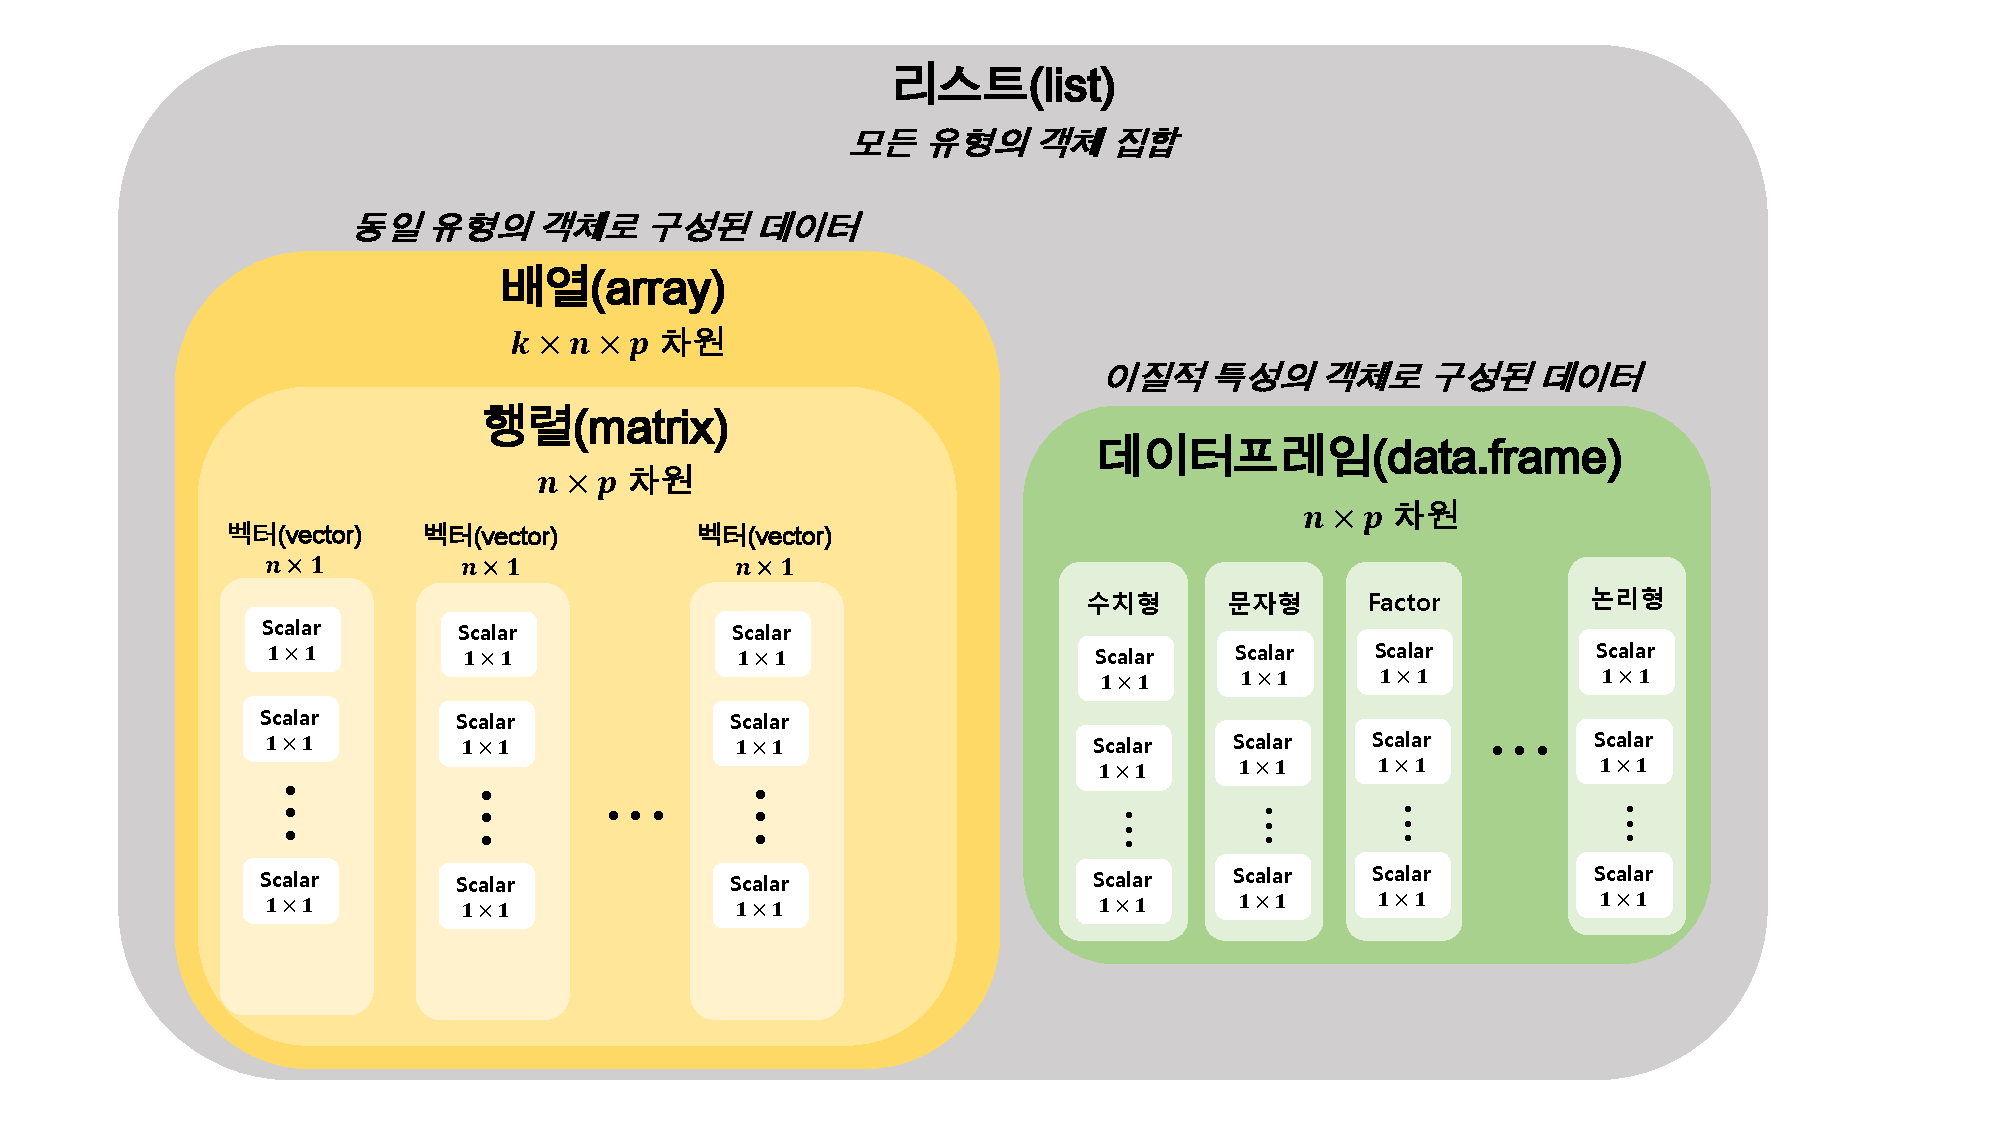
\includegraphics[width = 15cm, height = 14cm]{Figures/datatype-diagram}
  \caption[R 데이터 타입 구조 다이어그램]{R 데이터 타입 구조 다이어그램: R, Python 분석과 프로그래밍 (by R Friend)에서 발췌 후 수정}\label{fig:R-datatype}
} \end{figure}

\vspace{1cm}

\chapter{데이터 조작 I: 기본 자료 조작}\label{--i---}

\begin{quote}
\colorbox{gray!10}{\begin{minipage}{15cm}
\textbf{목적}
\begin{itemize}
  \item 기초적인 자료 입출력 방법 숙지
  \item 예시 자료를 이용한 자료 조작 
\end{itemize}
\end{minipage}}
\end{quote}

\section{데이터 처리 예시를 위한 실습 자료 설명}\label{------}

\subsection{Iris dataset}\label{iris-dataset}

\begin{itemize}
\tightlist
\item
  영국 통계학자 Ronald Aylmer Fisher가 소개한 데이터로 붓꽃의 세 가지
  종(setosa, versicolor, virginica)에 대해 꽃받침(sepal)과 꽃입(petal)의
  길이(length)와 너비(width)를 정리한 자료
\item
  지도 학습(supervised learning) 또는 비지도 학습(unsupervised learning)
  예시 자료로 유명
\item
  R의 기본 dataset에 포함되어 있으며 \texttt{data(iris)}로 자료 불러오기
  가능
\item
  Iris dataset의 구조
\end{itemize}

\footnotesize

\rowcolors{2}{gray!6}{white}

\begin{table}[H]

\caption{\label{tab:iris-desc}Iris 자료 설명}
\centering
\begin{tabular}[t]{lll}
\hiderowcolors
\toprule
변수명 & 설명 & 타입\\
\midrule
\showrowcolors
Sepal.Length & 꽃받침 길이 & numeric\\
Sepal.Width & 꽃받침 너비 & numeric\\
Petal.Length & 꽃잎 길이 & numeric\\
Petal.Width & 꽃잎 너비 & numeric\\
Species & 붓꽃의 종(setosa, versicolor, virginica) & factor\\
\bottomrule
\end{tabular}
\end{table}

\rowcolors{2}{white}{white}

\normalsize

\begin{itemize}
\tightlist
\item
  붓꽃 별 50행 씩 총 150행으로 이루어짐.
\end{itemize}

\footnotesize

\begin{Shaded}
\begin{Highlighting}[]
\KeywordTok{head}\NormalTok{(iris)}
\end{Highlighting}
\end{Shaded}

\begin{verbatim}
  Sepal.Length Sepal.Width Petal.Length Petal.Width Species
1          5.1         3.5          1.4         0.2  setosa
2          4.9         3.0          1.4         0.2  setosa
3          4.7         3.2          1.3         0.2  setosa
4          4.6         3.1          1.5         0.2  setosa
5          5.0         3.6          1.4         0.2  setosa
6          5.4         3.9          1.7         0.4  setosa
\end{verbatim}

\begin{Shaded}
\begin{Highlighting}[]
\KeywordTok{str}\NormalTok{(iris)}
\end{Highlighting}
\end{Shaded}

\begin{verbatim}
'data.frame':   150 obs. of  5 variables:
 $ Sepal.Length: num  5.1 4.9 4.7 4.6 5 5.4 4.6 5 4.4 4.9 ...
 $ Sepal.Width : num  3.5 3 3.2 3.1 3.6 3.9 3.4 3.4 2.9 3.1 ...
 $ Petal.Length: num  1.4 1.4 1.3 1.5 1.4 1.7 1.4 1.5 1.4 1.5 ...
 $ Petal.Width : num  0.2 0.2 0.2 0.2 0.2 0.4 0.3 0.2 0.2 0.1 ...
 $ Species     : Factor w/ 3 levels "setosa","versicolor",..: 1 1 1 1 1 1 1 1 1 1 ...
\end{verbatim}

\begin{Shaded}
\begin{Highlighting}[]
\KeywordTok{summary}\NormalTok{(iris)}
\end{Highlighting}
\end{Shaded}

\begin{verbatim}
  Sepal.Length   Sepal.Width    Petal.Length   Petal.Width        Species  
 Min.   :4.30   Min.   :2.00   Min.   :1.00   Min.   :0.1   setosa    :50  
 1st Qu.:5.10   1st Qu.:2.80   1st Qu.:1.60   1st Qu.:0.3   versicolor:50  
 Median :5.80   Median :3.00   Median :4.35   Median :1.3   virginica :50  
 Mean   :5.84   Mean   :3.06   Mean   :3.76   Mean   :1.2                  
 3rd Qu.:6.40   3rd Qu.:3.30   3rd Qu.:5.10   3rd Qu.:1.8                  
 Max.   :7.90   Max.   :4.40   Max.   :6.90   Max.   :2.5                  
\end{verbatim}

\normalsize

\subsection{Blood pressure dataset}\label{blood-pressure-dataset}

\section{외부 파일 입출력}\label{--}

\begin{quote}
\colorbox{gray!10}{\begin{minipage}{15cm}
\textbf{목적}

Excel 자료 저장 방식인 \texttt{.xls}, \texttt{.xlsx} 확장자 파일과 일반적인 텍스트 형태 자료 저장 방식인 \texttt{.txt}, \texttt{.csv} (콤마 분리 형식) 등과 같은 확장자를 가진 파일을 R workspace로 읽고, R에서 처리한 자료를 외부로 출력하는 방법을 습득한다. 

\end{minipage}}
\end{quote}

\subsection{RStudio에서 외부 파일 읽어보기}\label{rstudio---}

\begin{itemize}
\tightlist
\item
  최근 Rstudio version 1.1.xxx 이후 손쉽게 외부 자료를 R workspace 에
  불러오는 것이 가능해짐.
\item
  Rstudio 상단 메뉴에서

  \begin{itemize}
  \tightlist
  \item
    \texttt{{[}File{]}} \(\rightarrow\)
  \end{itemize}
\end{itemize}

\renewcommand\bibname{References}
\bibliography{CNUH.bib}


\end{document}
